\chapter{Accelerator Generation and Integration Using Program Binaries}
\label{instrumentChap}
As usability remains to be one of the most significant obstacles for adoption of FPGA computing, in this chapter, we explore the possibility of a user
transparent flow for mapping applications to systems with reconfigurable components.
In contrast to previous chapters where source code in high level
languages is used as input, here we try to only use the program binaries and their execution profiles as the design entries. 
The mechanism for integrating the accelerator back into the overall program execution is also discussed. 
%While our computational pipeline synthesis flow was to create better compute engines running on FPGA itself, in this chapter, we
%further discuss the interaction between the software component and the FPGA accelerators. 
From the users' perspective, a flow based on
program binaries requires no source rewriting
nor recompilation, the effort needed to take advantage
of the reconfigurable platform is thus minimized. 

With respect to the synthesis of the actual compute engine, we certainly take advantage of what we have developed in the previous chapters. 
The decoupled computational pipeline is again used as the architectural
template to which the original software behavioral descriptions are mapped. The overall performance of the hardware implementation is thus a net result of exploiting pipeline, memory level and coarse grained parallelism in the application, as will be described in later parts of this chapter.

%\section{Binary Analysis and Modification Infrastructure}
%As
%To find the loops, we use the DyninstAPI~\cite{dyninst} to parse through
%the program binaries and construct the control flow graph (CFG).
\section{Profiling Program Execution with Binary Instrumentation}
To perform various analysis on and eventually stitch the invocation of accelerators into the original program binary, we leverage the infrastructure developed in the field
of binary instrumentation. In particular, Dyninst~\cite{dyninst}  provides
great APIs for parsing, analyzing and modifying  program binaries, both statically and dynamically. 



\begin{figure}[htp]
\begin{center}
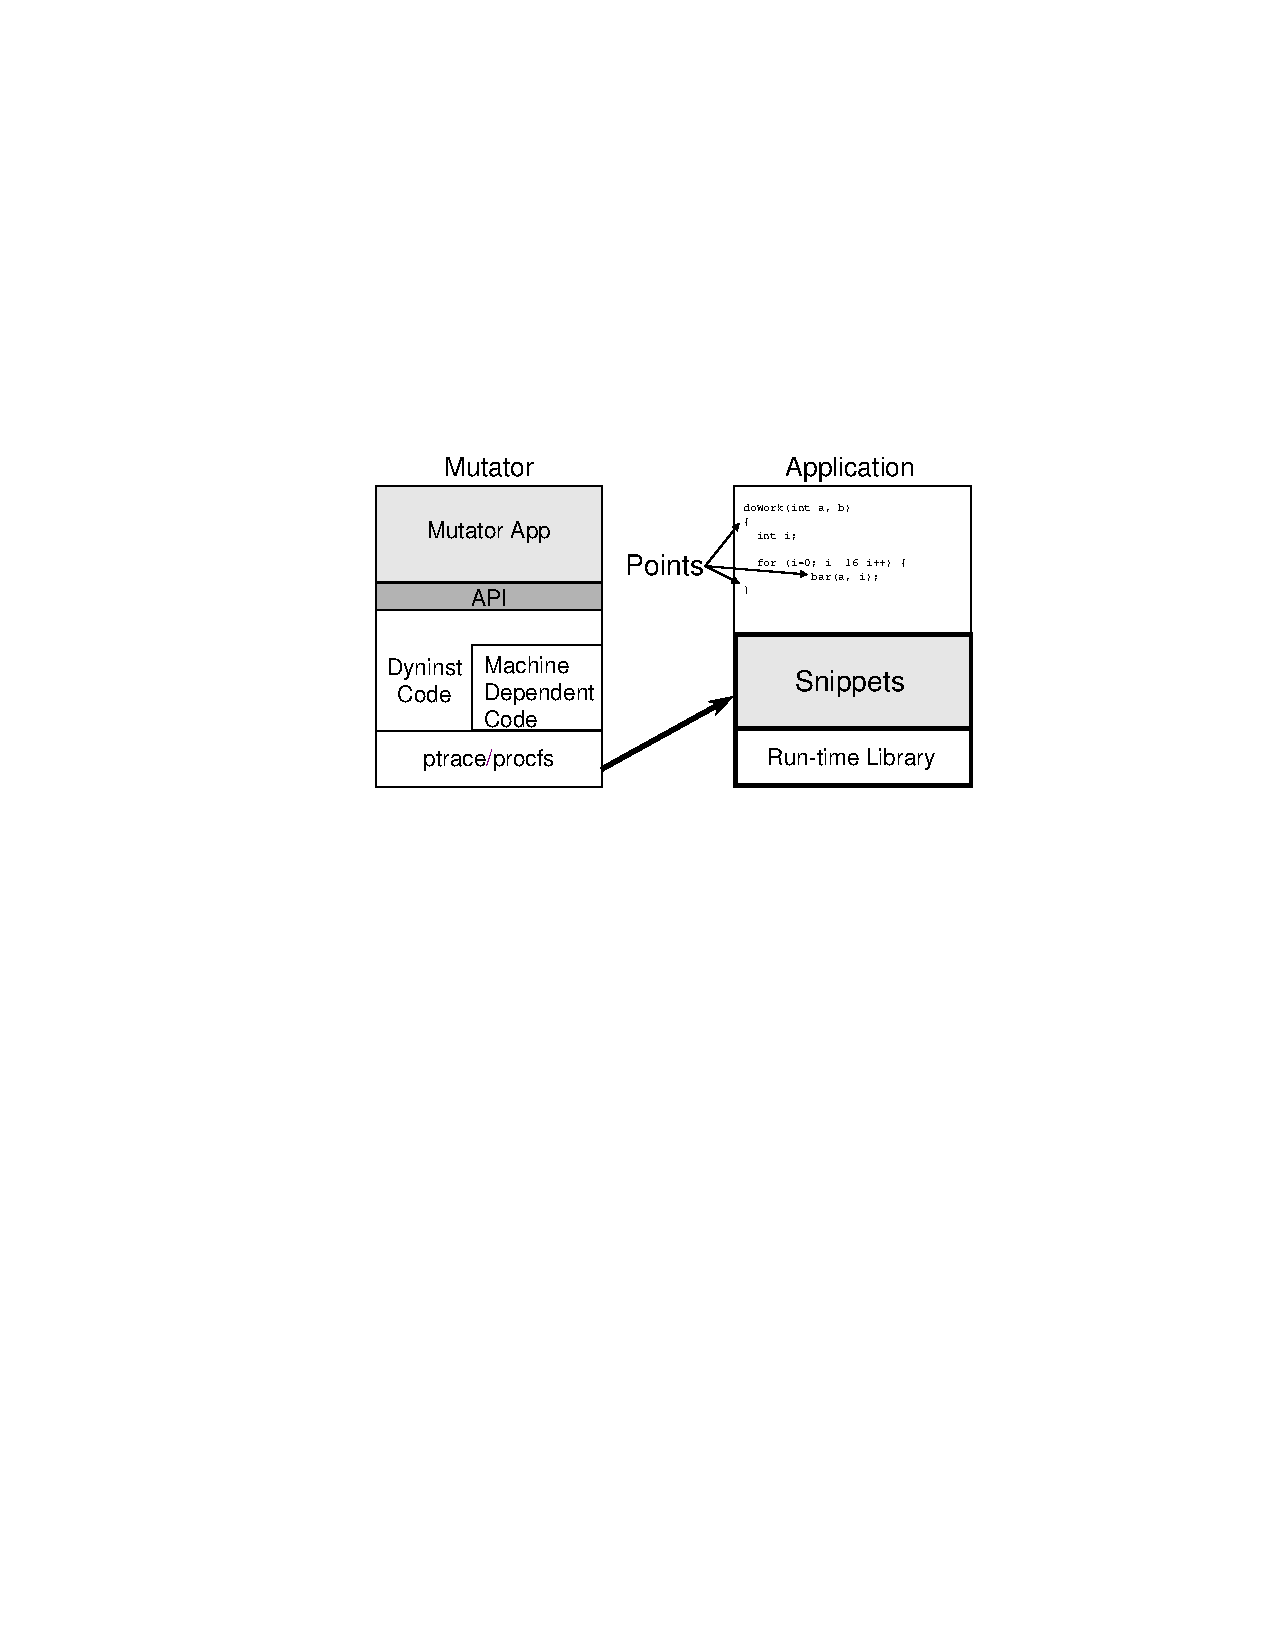
\includegraphics[width=0.6\linewidth]{chap6fig/dyninst.pdf}
\caption{Dynamic instrumentation in Dyninst~\cite{Buck:2000:ARC:1080622.1080630}
\label{dyninstAPIPic}}
\end{center}
\end{figure}


To capture useful information during the execution of a program, Dyninst's dynamic instrumentation functionality is used. Its overall implementation is shown
in figure~\ref{dyninstAPIPic}. 
In Dyninst's terminology, the binary to be modified is called the ``mutatee" while the program performing the instrumentation is the ``mutator". Code that gets inserted
into a program binary is organized into ``snippets".
The OS services used by debuggers (e.g., ptrace, /proc filesystem, etc.) are employed by the mutator to control process execution and to read and write the
address space of the mutatee program. Dyninst also has a dynamic linked library
which contains utility functions and two large arrays. With this library loaded
into the mutatee application, the arrays can be used for dynamically allocating small regions of memory. The instrumentation variables and code are stored separately among the two arrays. The snippets are first translated into machine code in the memory of the mutator process and then copied into the array in the mutatee address space. The original code is then modified to branch to the newly generated code. 

It's worth noting that the insertion and deletion
of snippets can all be done dynamically during runtime. A mutator can attach to a running process to add information-gathering snippets, and after enough data is collected, remove all instrumentation and detach itself.
The overhead of profiling is therefore only transient when applied to a long running program. Even though the performance may degrade to various extents depending on the actual snippets added, the application doesn't have to be interrupted.

Given Dyninst's capability, we can insert counters, track memory addresses referenced and log register accesses at points of interest in the program. It helps us
identify the most frequently executed loop nests in the applications and allows us to capture all necessary information to perform the analysis and parallelization described in the later sections. 







\section{Characteristics of the Targeted Platform}
\label{chartarg}
The general approach of translating program binaries to accelerators can certainly be applied to various heterogeneous platforms. To justify some of the design decisions made in our flow, the assumed platform 
characteristics need to be outlined first. 
In section~\ref{hetero}, a whole array of machines with reconfigurable
components were examined and there is a wide spectrum of configurations
when it comes to how tightly integrated the reconfigurable fabric is to
the processor. 
In this work, we focus on the part of the space where the general purpose processor and the reconfigurable component are loosely coupled.
Instead of being a functional unit in the processor
execution pipeline, the FPGA is used as a coprocessor for which
communication and management is assumed to be expensive.
Meanwhile, the capacity of the reconfigurable fabric can potentially be greater as it is not constrained in any way by the pipeline of the associated processor. 
Most of the off-the-self systems currently available or in development~\cite{xeonwithfpga} fall into this category. As the
costs of semiconductor manufacturing become prohibitive, 
special processors with modified pipeline accommodating
reconfigurable functional units are less likely to be built
and offered commercially, as compared to systems with conventional
processor and FPGA integrated at either chip, package or board level.

Another important factor to consider is how sharable the memory
is between the CPU and the FPGA. 
One possible configuration, as represented by the zynq SoC, has
the CPU's address space shared with the programmable logic.
The physical addresses used to access the memory are identical,
whether it comes from the CPU or the FPGA. Of course in the presence
of virtual memory, address translation needs to occur
before the requests are forwarded to the memory subsystem. On the other hand, there are
platforms where the FPGA has its own memory space which is
explicitly populated with the working dataset before the activation of 
the accelerator~\cite{sdaccel}. It's worth noting that this difference in programming model
is orthogonal to the actual physical configuration of the platform. For instance, CPU and FPGA located in two different sockets can have shared address space while a system based on a single chip SoC may associate the FPGA with a separate DRAM interface which are not directly
accessible by CPU. 
Given the flexibility of FPGAs, there are certainly ways to create a layer of abstraction conforming to either one of these schemes, regardless
the original expected usage model. 
In this work, we assume a shared memory space between the CPU and the FPGA, which
is one of the properties of the experiment platform we use, though a mechanism for explicit data movement applicable in non-shared memory system is also discussed in section~\ref{dtransfer}.

%However in this work, because of the nature
%of our targeted applications, we are able to devise mechanisms to tackle explicit data

%we 
%do not make assumption about the underlying platform and try to
% devise a mechanism for each scheme. 
%we treat these
%two schemes differently, as will be discussed in section~\ref{makingAcc}.
%Finally, in any CPU+FPGA coprocessor systems, the access of data memory by the programmable logic can be seen as adding to the communication overhead between the
%accelerated part and the software components, which is a key parameter
%in determining if a part of the program should be accelerated using hardware.





%To find the loops, we use the DyninstAPI~\cite{dyninst} to parse through
%the program binaries and construct the control flow graph (CFG).





\section{Acceleratable Regions In Program Binaries}
The trade-off between communication efficiency and capacity
in the reconfigurable components of the systems dictates
the granularity of the accelerators to be synthesized. 
Given the loose coupling between the programmable logic and the processor,
while it is still possible to create accelerators for small windows of dynamic instruction stream, the cost of frequently controlling and communicating
with these tiny hardware engines would nullify any performance gain
achieved. 
It is ideal to have a relatively large chunk of computation
handed off to the FPGA, which then works independently with little
intervention from the CPU, before signalling the completion of the task.
The natural targets for our flow are therefore loop nests in the program
binaries. There may be cases where code segments are shared by multiple loops, making it harder to statically carve out the best code region for acceleration. For these
scenarios, we can leverage runtime profile of the program to find the prevalent
loops and extract single-entry-multiple-exit loops which can undergo further
optimizing transformations. 
Meanwhile, due to the presence of statically unresolvable control flow, e.g. indirect jump,
not every part of the program can be analyzed. Several techniques were
proposed to tackle this in dynamic binary translation~\cite{Hiser:2007:EIB:1251974.1252530}, which we can potentially
adopt. However, we do not aim to have complete coverage of the code as only the
computation heavy loops are of interest to us.
Practically speaking, the more regular loops, which are the ideal candidates for FPGA acceleration, are generally easy to detect and analyze. 
% The accelerator will be invoked only if the execution 


Another characteristic of the FPGA platform is its low clock frequency
(as compared to a typical CPU), thus to have significant speed up, there
needs to be substantial amount of parallelism extracted, which requires large windows of instruction.
In addition to instruction level parallelism within basic block or a single iteration of a loop, coarse grained parallelism 
%spanning the iteration space of loop nests 
also needs to be exploited. Blocks of loop iterations are to be executed in parallel, which implies very aggressive instruction
reordering when the accelerators are created.
%
%Meanwhile, the aggressive reordering of these instructions in creating the %accelerator
%makes any speculative execution very expensive. 
Consequently, speculative execution, which some binary-based dynamic parallelization techniques were based on, may become rather expensive. As states generated by the speculatively performed operations need to be buffered, 
the amount of space required to accommodate the massively parallel execution engine
%exploited
can be large.
The subsequent commit of these states may also induces long delays
or requires complicated hardware mechanism.
In particular, for any speculatively disambiguated memory accesses, the address streams need to be dynamically cross compared to ensure the
reordering of loads and stores are indeed valid. 
Using past execution profile can boost the confidence with which the disambiguation
is performed, but the probabilistic nature of the approach does not
relieve us the need for costly dynamic checking mechanisms. To generate
lean and fast accelerators, in this work, we try to extract a set of conditions for parallelization which does not vary with the amount of work
in the loop. In other words, we want to find computation that can 
be done during run time with a fixed, statically known cost, yet still guarantees the validity of the instruction reordering we have performed for accelerator generation. 
%This will allow us to quickly gauge if an instance of a loop nest should be executed on hardware.

\subsection{Dependencies in Loops}
To understand what characteristics a loop nest should manifest for it to be a feasible target, it is useful to start from the theory of loop dependencies. As
explained in section~\ref{sec:partins}, statements cannot be parallelized or
reordered when there are RAW, WAR or WAW dependencies between them. In the context of instructions in loop nests,~\cite{Kennedy:2001:OCM:502981} defined
loop-carried and loop-independent dependencies between a pair of statements $S_1$ and $S_2$ (at least one of which is writing to memory):
\begin{itemize}
    \item loop-carried dependency: $S_1$ accesses a memory location 
    on one iteration of a loop, and $S_2$ accesses the same location on a subsequent iteration. 
    \item loop-independent dependency: $S_1$ and $S_2$ access the same memory location in the same loop iteration, and there is a execution path from $S_1$ to $S_2$. 
\end{itemize}
The concepts of \textit{iteration number}, \textit{iteration vector} and \textit{iteration space} were also introduced. The iteration number is the 
index number for a particular loop iteration, while the iteration vector
extends this concept to a multi-level loop nest. Each element in the vector
corresponds to one level in the loop nest with the left most element representing the outermost loop index. The set of all possible iteration vectors then
constitutes the iteration space. Figure~\ref{fig:inivis} visualizes these concepts with a simple loop nest. 

\begin{figure}[htp]
\begin{center}
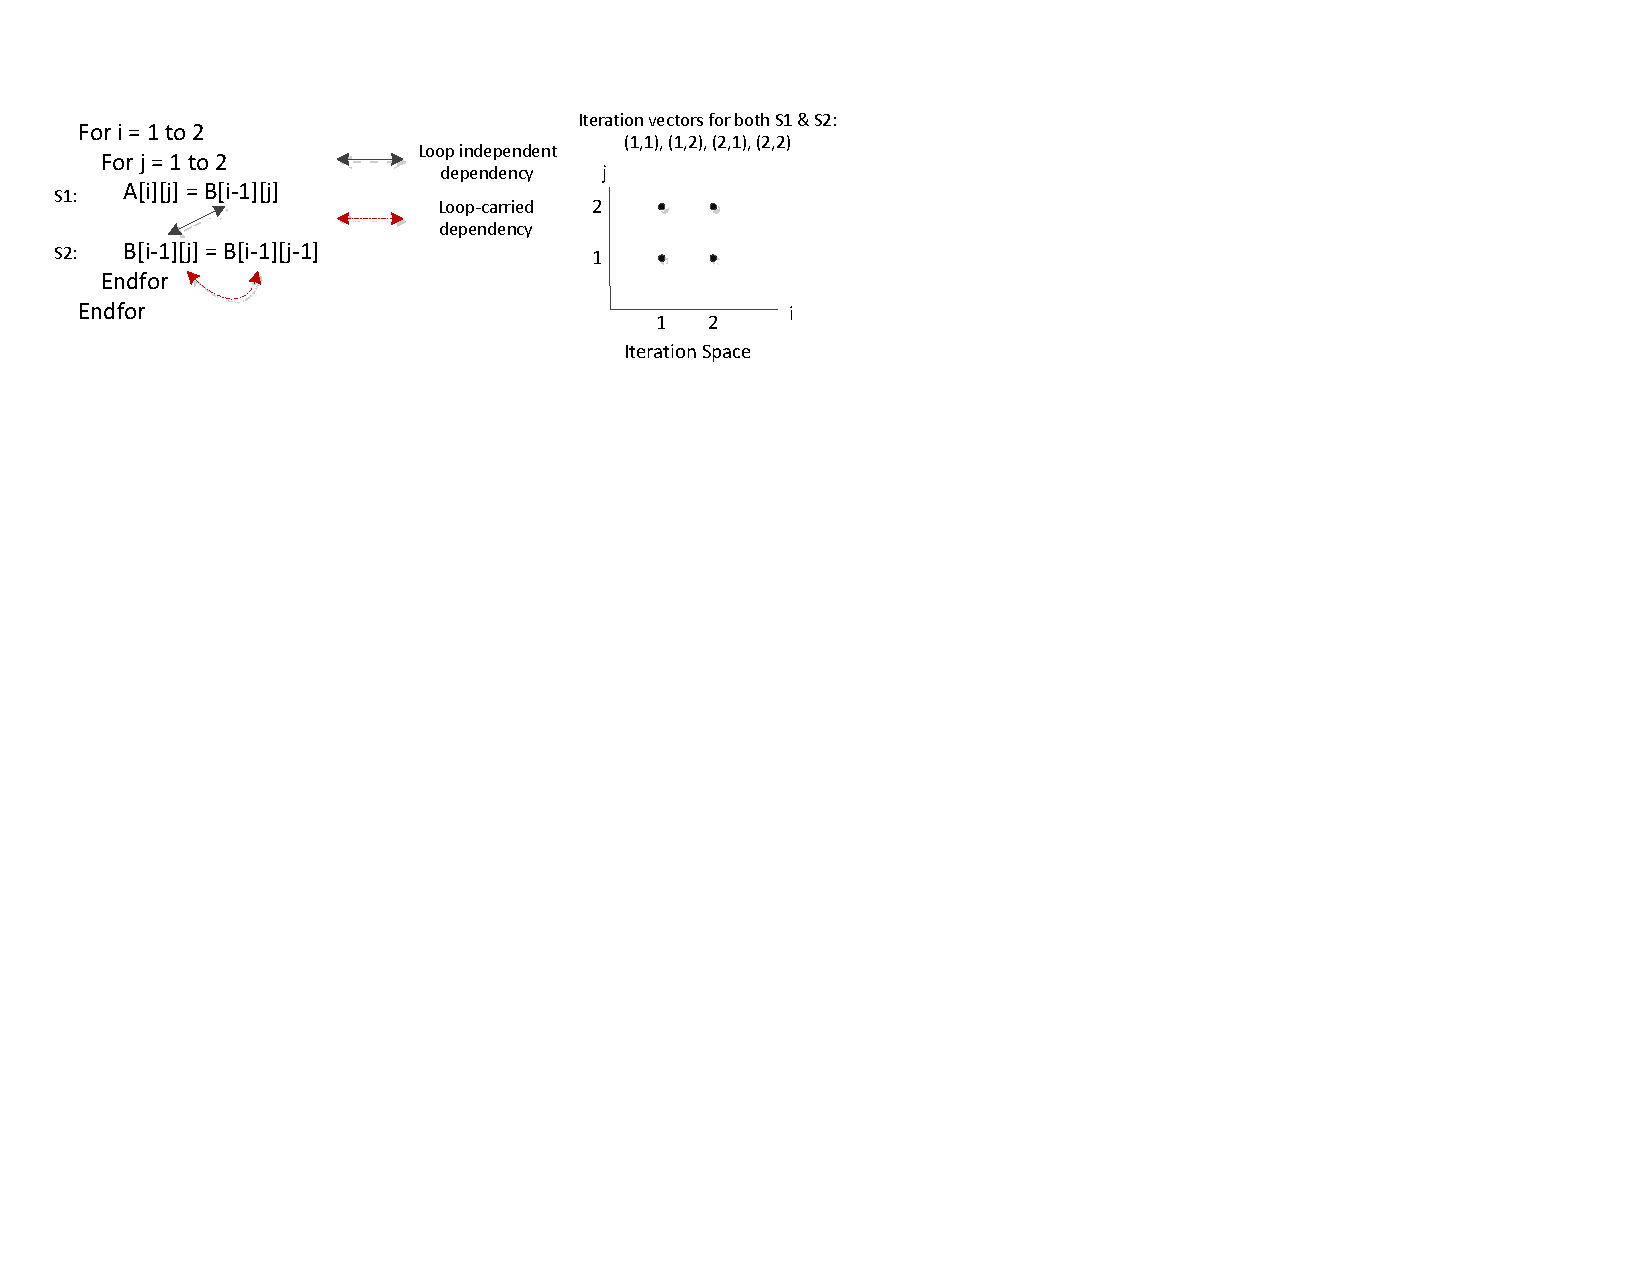
\includegraphics[width=0.9\linewidth]{chap6fig/iterationSp.pdf}
\caption{Dependencies in a Loop Nest
\label{fig:inivis}}
\end{center}
\end{figure}

To exploit coarse grained parallelism in the loop nest, we need to ensure the
absence of loop carried dependencies at a particular level in the loop nest. There are also simple transformations(e.g. loop interchange) which can move loop carried
dependencies to other loop levels so only loop-independent dependencies are left. To enable the discovery of these opportunities, we need to find, in each statement's iteration space, if they intersect with other statements' accessed memory locations. In general, the memory addresses to be accessed can be arbitrary functions of loop indices and run time data, which makes it impossible to statically determine if
dependencies exist. There are, however, a  set of problems where
the memory referenced can be analyzed during compile time as the addresses are affine functions of the loop index variables. For loop nests of this kind,
dependency analysis is essentially finding integer solutions for the problem:

\begin{equation}
\begin{aligned}
\label{dioeq}
& \text{} & & f(\vec{x}) = h(\vec{y}) \\
\end{aligned}
\end{equation}
\begin{equation*}
\begin{aligned}
& \text{ where}  & & f(\vec{x}) = a_0 + a_1x_1+...+a_nx_n \\
& & & h(\vec{y}) = b_0 + b_1y_1+...+b_ny_n \\
& & & \vec{x}_{lb} \le \vec{x} \le \vec{x}_{ub} \\
& & & \vec{y}_{lb} \le \vec{y} \le \vec{y}_{ub}
\end{aligned}
\end{equation*}
Or equivalently this linear Diophantine equation:
\begin{equation}
\begin{aligned}
\label{adioeq}
a_1x_1-b_1y_1+...+a_nx_n-b_ny_n = b_0 - a_0
\end{aligned}
\end{equation}
\begin{equation*}
\begin{aligned}
& \text{ where}  & & x_{lb_k} \le x_k \le x_{ub_k} \\
& & & y_{lb_k} \le y_k \le y_{ub_k} \\
\end{aligned}
\end{equation*}

Both function $f$ and $h$ takes a iteration vector from within the iteration space of the statement, point-wise bounded by $\vec{x}_{lb}/\vec{y}_{lb}$ and $\vec{x}_{ub}/\vec{y}_{ub}$, and map it to a memory location. When
multi-dimensional arrays are used, variables can be separated such that
we have multiple simultaneous equations which are simpler to solve.
The loop carried dependency in figure~\ref{fig:inivis}, for instance, correspond to the following equations:
\begin{equation*}
\begin{aligned}
-1+x_1 = -1+y_1 \\
x_2 = y_2-1 \\ 
\end{aligned}
\end{equation*}
\begin{equation*}
\begin{aligned}
& \text{ where}  & & 1 \le x_1 \le 2 \\
& & & 1 \le x_2 \le 2 \\
& & & 1 \le y_1 \le 2 \\
& & & 1 \le y_2 \le 2 \\
& & & x_1,x_2,y_1,y_2 \in Z
\end{aligned}
\end{equation*}


This problem is an integer linear program, one of the NP-complete problems.  
There are various techniques~\cite{Ban76}~\cite{Banerjee:1988:DAS:535430}, proposed over the years, to efficiently solve a relaxed version of this problem. 
%can be used to compute if
%dependencies exist between memory references. Essentially they are all trying %to find solutions for the problem:
%Many techniques were proposed for compiling these problems onto variable %processors. 
In our binary-based flow, we also try to target these analyzable loop nests, some of which are especially amenable to FPGA acceleration. 
Identifying these regions from the program binaries, however, poses some challenges. 
%however, is not as
%simple as doing it from the source code.


%This can be done by solving the

%direction vector
%is the way to do it
%To capture the dependencies between statements, \texit{direction vector} are computed between statements.

\subsection{Challenges for Binary-based Analysis}
\label{sec:cfbba}
The regular and analyzable memory access patterns expressed in high
level languages become rather mangled when the program binaries are 
being examined. All memory accesses are pointer based with no high
level information to indicate if the data structures they are targeting
are disjoint. With dimensionality of the arrays eliminated, 
separate variables in original address calculation are now coupled to each other. In essence, we have to perform dependency analysis on a huge linear
array with all addresses being the result of some run time computation.
Figure~\ref{fig:mangledMem} illustrates how different a
set of memory accesses manifest themselves in the actual high level source code v.s. program binaries.

\begin{figure}[htp]
\begin{center}
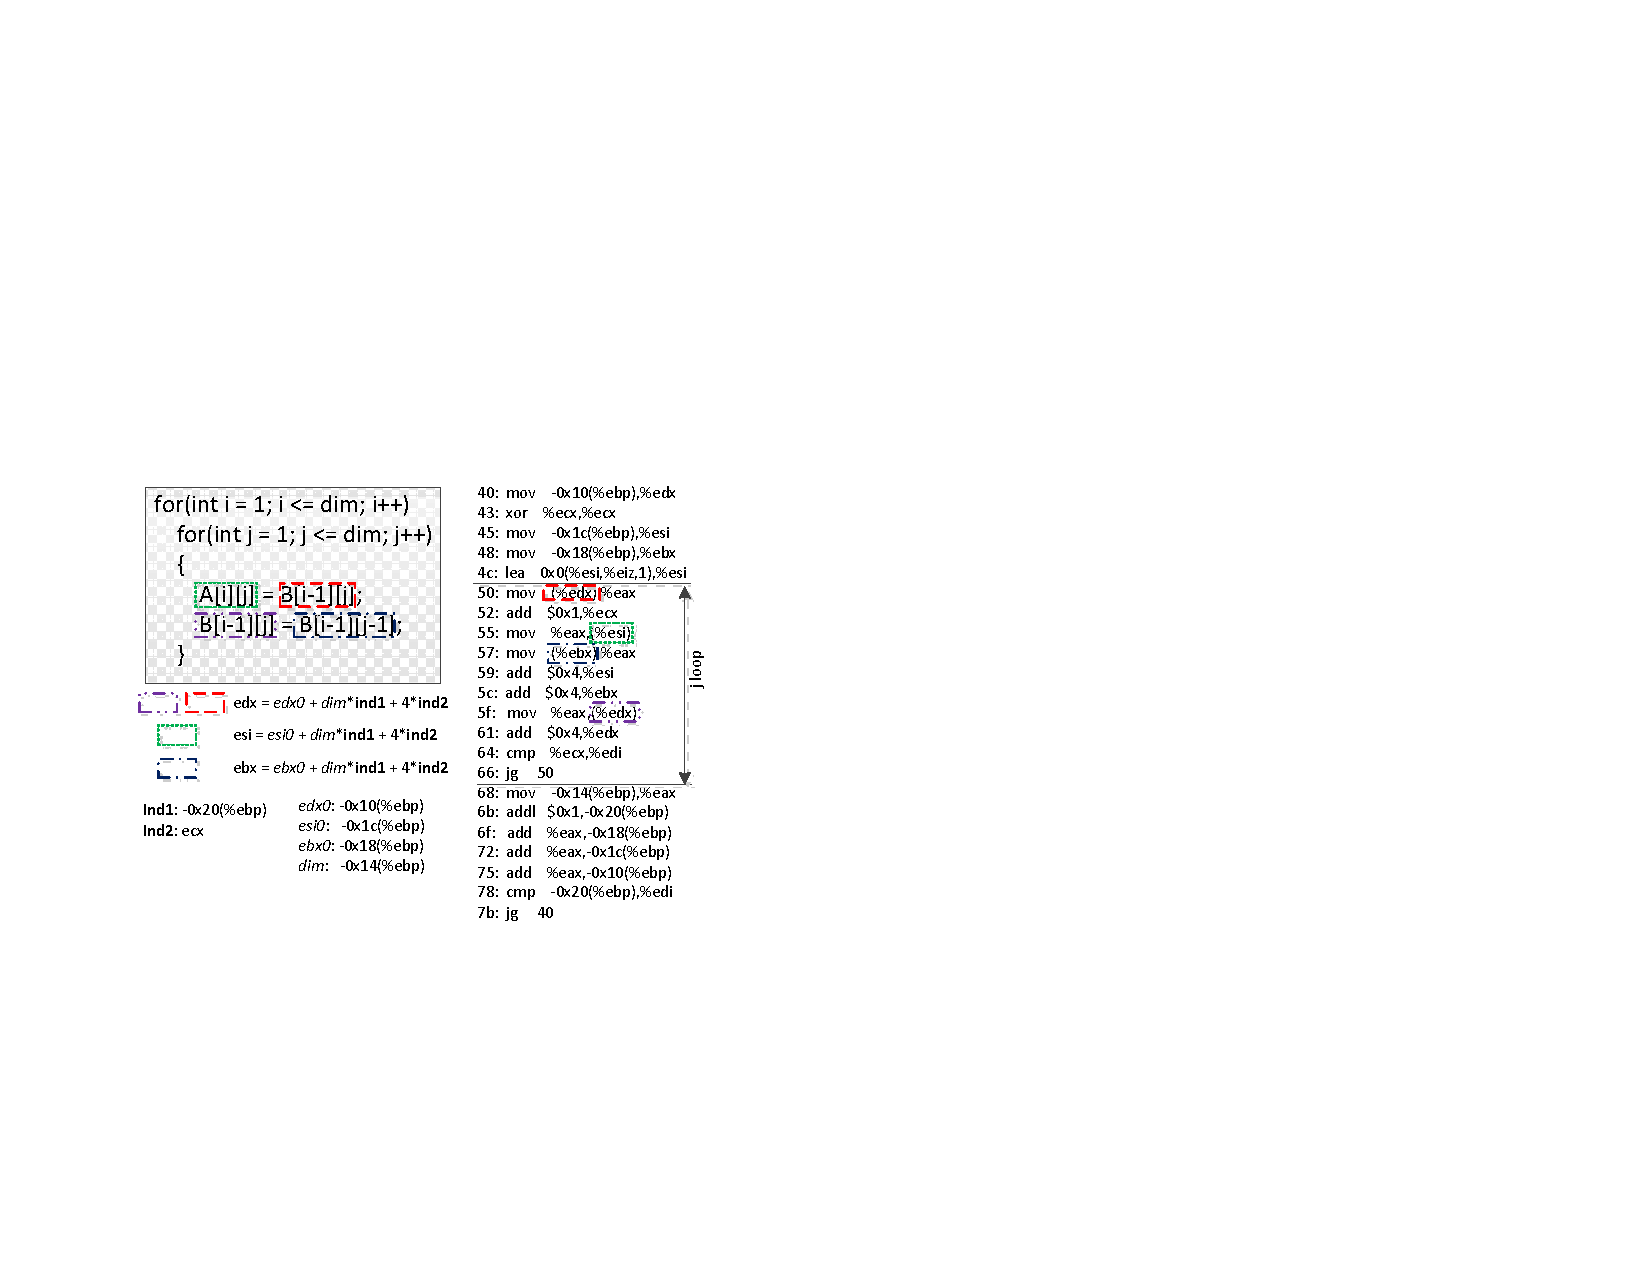
\includegraphics[width=0.8\linewidth]{chap6fig/memBin.pdf}
\caption{Memory Accesses in Program Binaries
\label{fig:mangledMem}}
\end{center}
\end{figure}

In this example, even though the original array references are all affine functions of the loop index variables, in the program binaries, their calculation is much more complex. 
Dependency testing involving only a single loop index in the source code now have to deal with multiple induction variables. More importantly, for equation~\ref{adioeq}, the coefficients ($a_0...a_n$ and $b_0 ... b_n$) are statically known constants while
in the binaries, everything is a runtime data item stored in either a register or a memory location. Naively 
substituting these symbolic variables into the Diophantine's equations yields
a non-linear formulation which can not be solved by the common techniques
in optimizing compilers. On the other hand, %it is relatively straight forward, 
as long as these coefficients are unchanged during the execution of the loop nests, we can use past execution profile to extract these numbers, perform analysis and carry out parallelization. Meanwhile, as the assumed parallelism is based on past behaviors, we need to leverage various classic dependency testing techniques to formulate a set of checks to be performed during run time as well. The cost of these check, however, is fixed. The dependency
analysis problem does not scale up with the number of iterations, but rather the number of levels in the loop nest, which is easily recognizable from the static binaries. We can therefore quickly verify our coarse grained parallelization before the invocation of the accelerator, 
avoiding speculative execution and the associated costs. 

In our flow, dataflow analysis is always performed on loop nests to ensure there are no updates to these coefficients during the loops' execution, before more detailed dependency testing and parallelization are attempted. The  potential for actual speed up of course largely depends on the existence of memory level and coarse grained parallelism.



%we can be sure that only a fixed amount of computation is needed in
%the dependency. This is not hard to see as the size of the problem formulated 
%does not depend on the actual values of the variable but the number of levels in the loop nest.

%we can assume they are runtime constant and the dependency analysis
%can be carried out. 



%Our approach to deal with this uncertainty is described later in section~\ref{makingAcc}.





\subsection{From Dependency Testing to Parallelization}
\label{sec:fdtp}
%With the dependency testing done, we need to examine the loop nests' potential for parallelization.

To identify the opportunities in parallelizing a loop nest, the $dependency$ $distance$ $vectors$ and $direction$ $vectors$~\cite{opac-b1000180} are used.
%One way to bridge this gap is through the use of distance and direction vectors~\cite{opac-b1000180}. 

\begin{figure}[htp]
\begin{center}
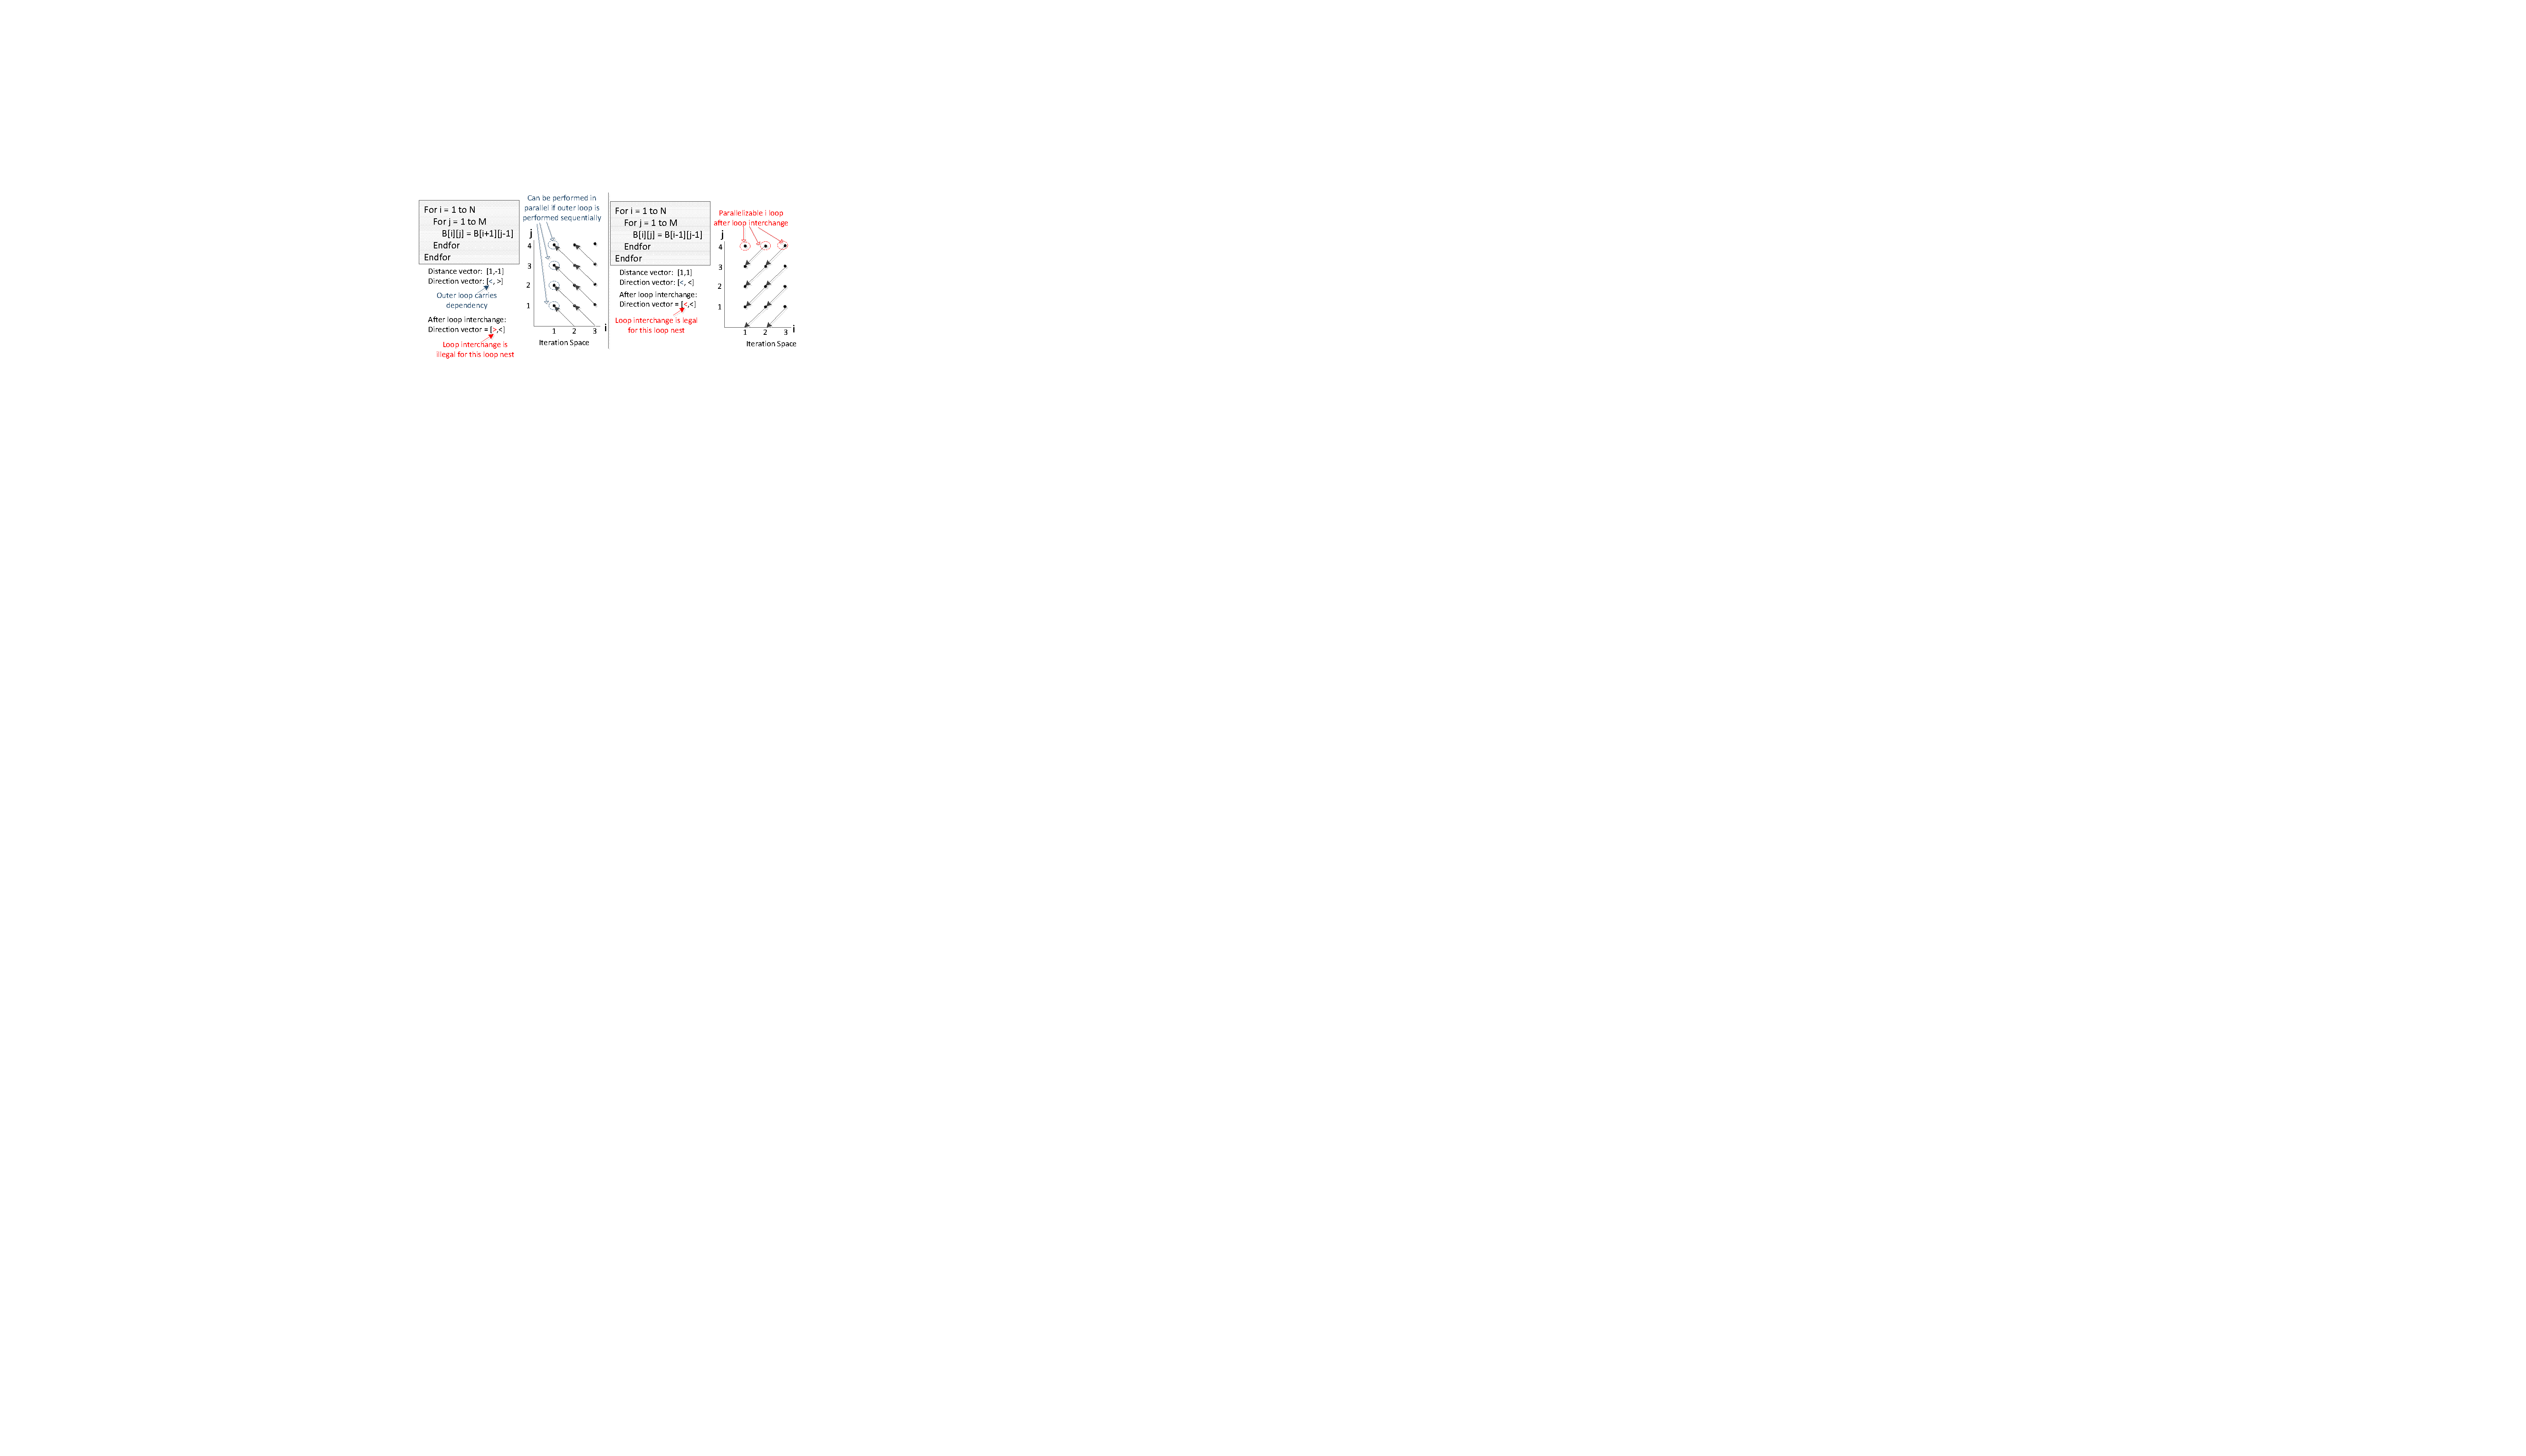
\includegraphics[width=1.0\linewidth]{chap6fig/paral2.pdf}
\caption{Parallelization with Direction Vectors
\label{fig:paral}}
\end{center}
\end{figure}
The $dependency$ $distance$ $vectors$ can be computed:
\begin{equation*}
\begin{aligned}
&  & & \vec{d}(\vec{x},\vec{y}) = \vec{y}-\vec{x} \\
& \text{ where }&   & \vec{x} \text{ and }\vec{y} \text{ are solutions to equation~\ref{dioeq}}  
\end{aligned}
\end{equation*}

These vectors give rise to the $direction vectors$ $D(\vec{x},\vec{y})$:
\begin{equation*}
\begin{aligned}
  & & ``<" \text{ if } \vec{d}(\vec{x},\vec{y})_k>0 \\
 \vec{D}(\vec{x},\vec{y})_k = &   & ``=" \text{ if } \vec{d}(\vec{x},\vec{y})_k=0\\
 & & ``>" \text{ if } \vec{d}(\vec{x},\vec{y})_k<0
\end{aligned}
\end{equation*}


The convention is to have the lexicographically earlier iteration vector to be
$\vec{x}$ and with that the leftmost non-``=" element of a direction vector would always be ``$<$". 
The index for this leading ``$<$" is also the level of the  loop-carried dependency. 
Assuming a transformation $T$ does not violate loop-independent dependencies,
~\cite{Kennedy:2001:OCM:502981} proved that $T$ is valid as long as
it does not cause some of the direction vectors to have ``$>$" as the leftmost non-``=" component. In addition, any iteration reordering at a level of the loop not carrying dependency is also valid. Using these proven theorems, we can
decide if loop transformations and iteration parallelization are legal when we know all the direction vectors of a loop nest. Figure~\ref{fig:paral} illustrates a
few scenarios where dependency direction vectors are used to determine validity
of transformation/parallelization.








%To summarize, our flow targets loop nests whose direction vectors can be extracted and coarse grained parallelism identified.



\begin{comment}

we leverage several techniques for taking advantage of the discovered parallelism. For the inner most loop, loop pipelining is always applied
to 

Assuming a particular loop level does not carry dependency, 

Comparing against other parallel computers such as multicore or SIMD machines, the 

Parallelization in FPGA vs others:
vectorization ? separate thread? loop pipelining? 


In order to get the dependency vector however, the memory access patterns would
need to be analyzable. Techniques for extracting dependency vectors were outlined in the .... These techniques generally require the array references
to be affine functions of the loop indices, where the coefficients are
all constants. 
Unfortunately, in the case of accelerating binaries, the coefficients are 
always variables stored in either register or a memory location. Naively
substitutes these variable into the Diophantine's equations yield
non linear conditions...As a result, even if the underlying computation are parallelizable, it is a lot harder to verify with the program binaries
as the starting points. It is relatively straight forward, however,
to detect if these coefficient are changed during the execution of the loop nests. 
\end{comment}

% we want something analyzable ---- % but of course even if the source code
% is analyzable, the binary may not be


\begin{comment}
Schemes for checking 
%

This is certainly compatible with the how conventional FPGAs are used
in most applications, where entire compute intensive loops are offloaded
and sped up.

Even as we focus on speeding up loops with large iteration count,
certain loop nests are just difficult to accelerate using FPGAs.
%especially
%when all higher level information is stripped away, as is the case with program binaries.
Due to the slower frequency of FPGA accelerators, it is not sufficient to just exploit instruction level parallelism. For there to be any net gain
in performance, coarse grained parallelism at the loop level has
to be extracted. To establish independence between different loop iterations or perform transformation to extract coarse grain parallelism, the 
\end{comment}





\section{A Two Phased Approach for Accelerating Program Binaries Using FPGA}
\label{makingAcc}
As the accelerator synthesis, which also includes the traditional FPGA CAD flow,
can take hours to finish, it cannot be performed on the fly while the
program to be accelerated is waiting. The preceding step, when loop nests are transformed/parallelized, is therefore
also performed offline. 
%From the previously collected profiles, we need to obtain
%the direction vectors which help us extract parallelism of various kinds.
%We therefore have to obtain the direction vectors 
%before running the actual program. 
In this work, Banerjee's test~\cite{Ban76} is used to find the direction vectors used for the extraction of parallelism. Since the required coefficients for equation~\ref{adioeq} are obtained from past execution profiles, the dependency testing and parallelization performed during this \textit{offline phase} are  a reflection of the programs' past behavior. When the accelerator is actually running, the input data would have changed. The \textit{online phase} thus includes a mechanism to guarantee the 
semantics of the program is not violated by the reordering performed during
the accelerator synthesis. As we have mentioned in section~\ref{sec:cfbba},
a verifying function is invoked before the accelerator, ensuring the correctness
of the overall execution. 



This online phase test is also one of the reasons why we choose Banerjee's method for our dependency testing even though it is not the most accurate dependency testing method
available. The Banerjee's inequality tests for existence of any real solutions for the Diophantine's equations. Since it only tackles the non-integer relaxation of the ILP formulation, the results obtained are conservative.
It will never report lack of dependencies when one exists,  but may report false dependencies, i.e. when all the real solutions are non-integral.
 More accurate tests like the Omega test~\cite{omega} find integer solutions but are more costly. Since we are
going to perform the test again using run time data when the accelerator is actually
being activated, the faster, though more pessimistic, method is preferred.

When applying Banerjee's method, a particular direction vector $\vec{v}$ is subjected to test, and the result reveals if a pair of memory accesses are dependent in $\vec{v}$'s direction. 
%first used as the constraint and the result of the test reports if this vector may hold true for a pair of memory accesses. 
%Therefore, 
To find all the direction vectors for dependencies, a hierarchy
of tests may therefore be involved. For a pair of memory accesses in a two level loop nest, the possible tests are shown in figure~\ref{fig:testingHier}, where ``$\ast$" denotes a union of ``$<$", ``=" and ``$>$". Negative test result from any node in the hierarchy eliminates the necessity to continue testing its subnodes. A subset of these dependency direction vectors
are true for each loop nest and dictates what kind of transformations are valid for accelerator synthesis.


\begin{figure}[htp]
\begin{center}
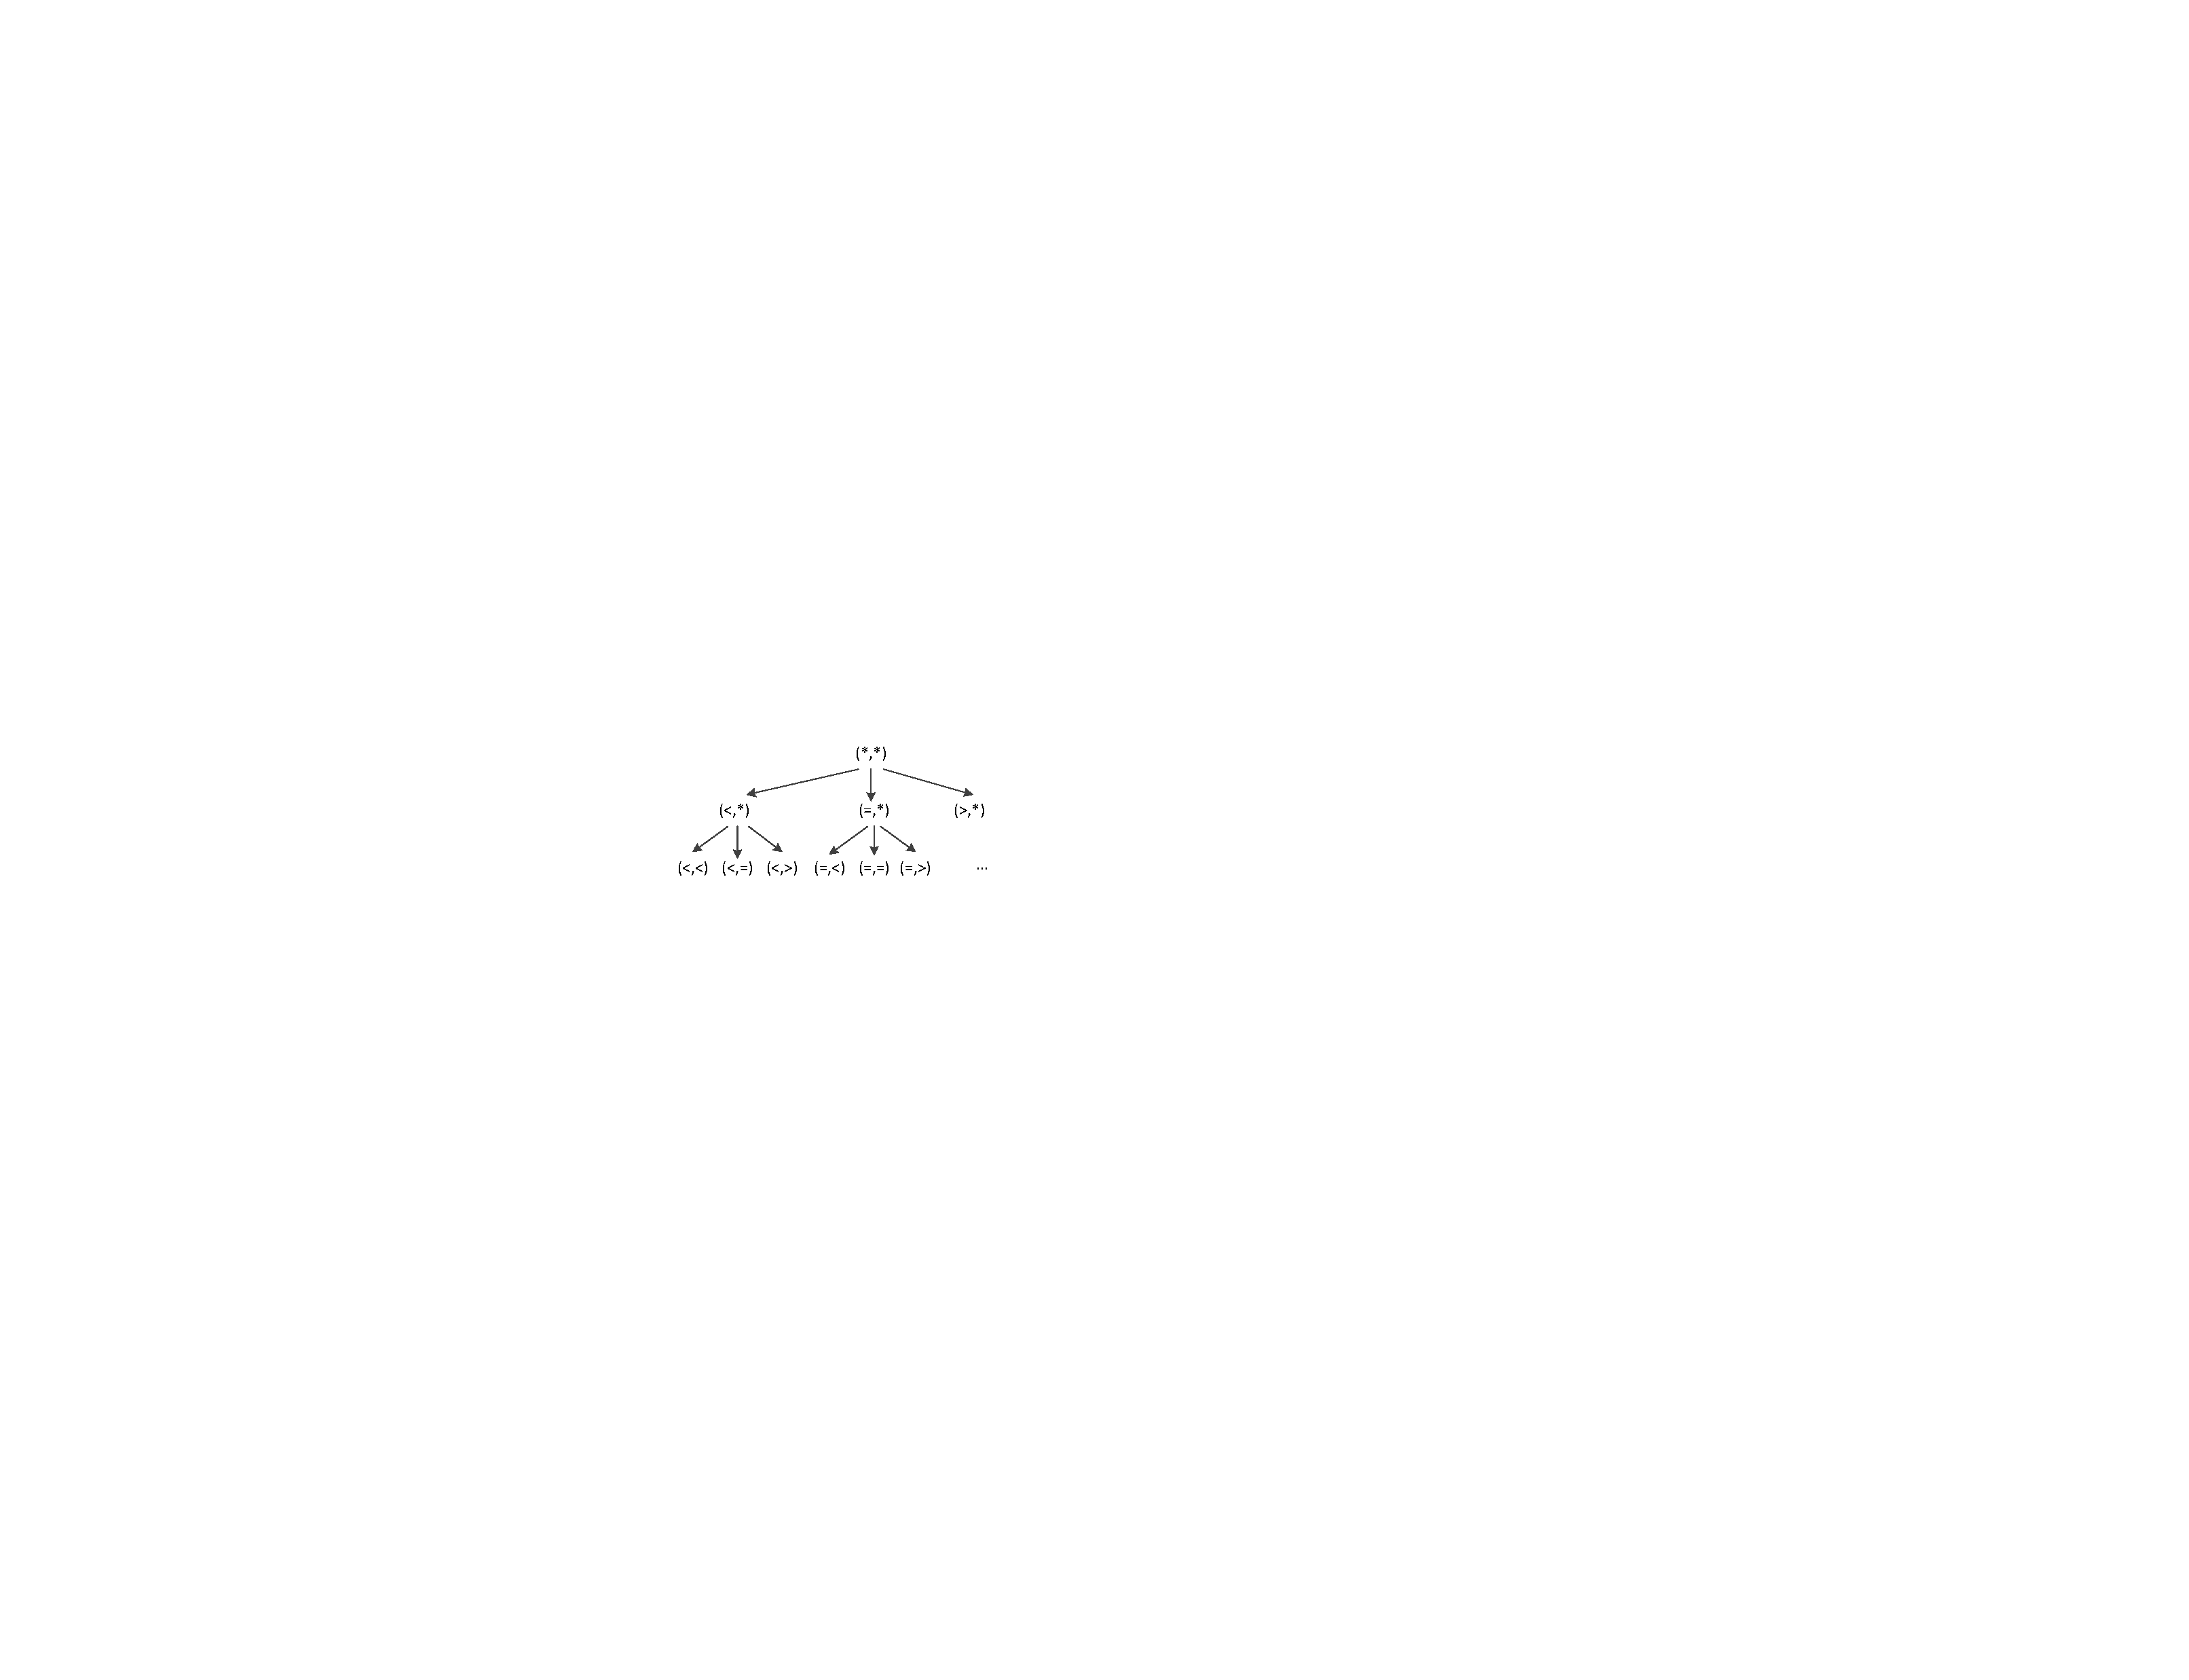
\includegraphics[width=0.6\linewidth]{chap6fig/testingHier.pdf}
\caption{Hierarchy of Dependency Testing for A Two-Level Loop Nest
\label{fig:testingHier}}
\end{center}
\end{figure}


\begin{figure}[htp]
\begin{center}
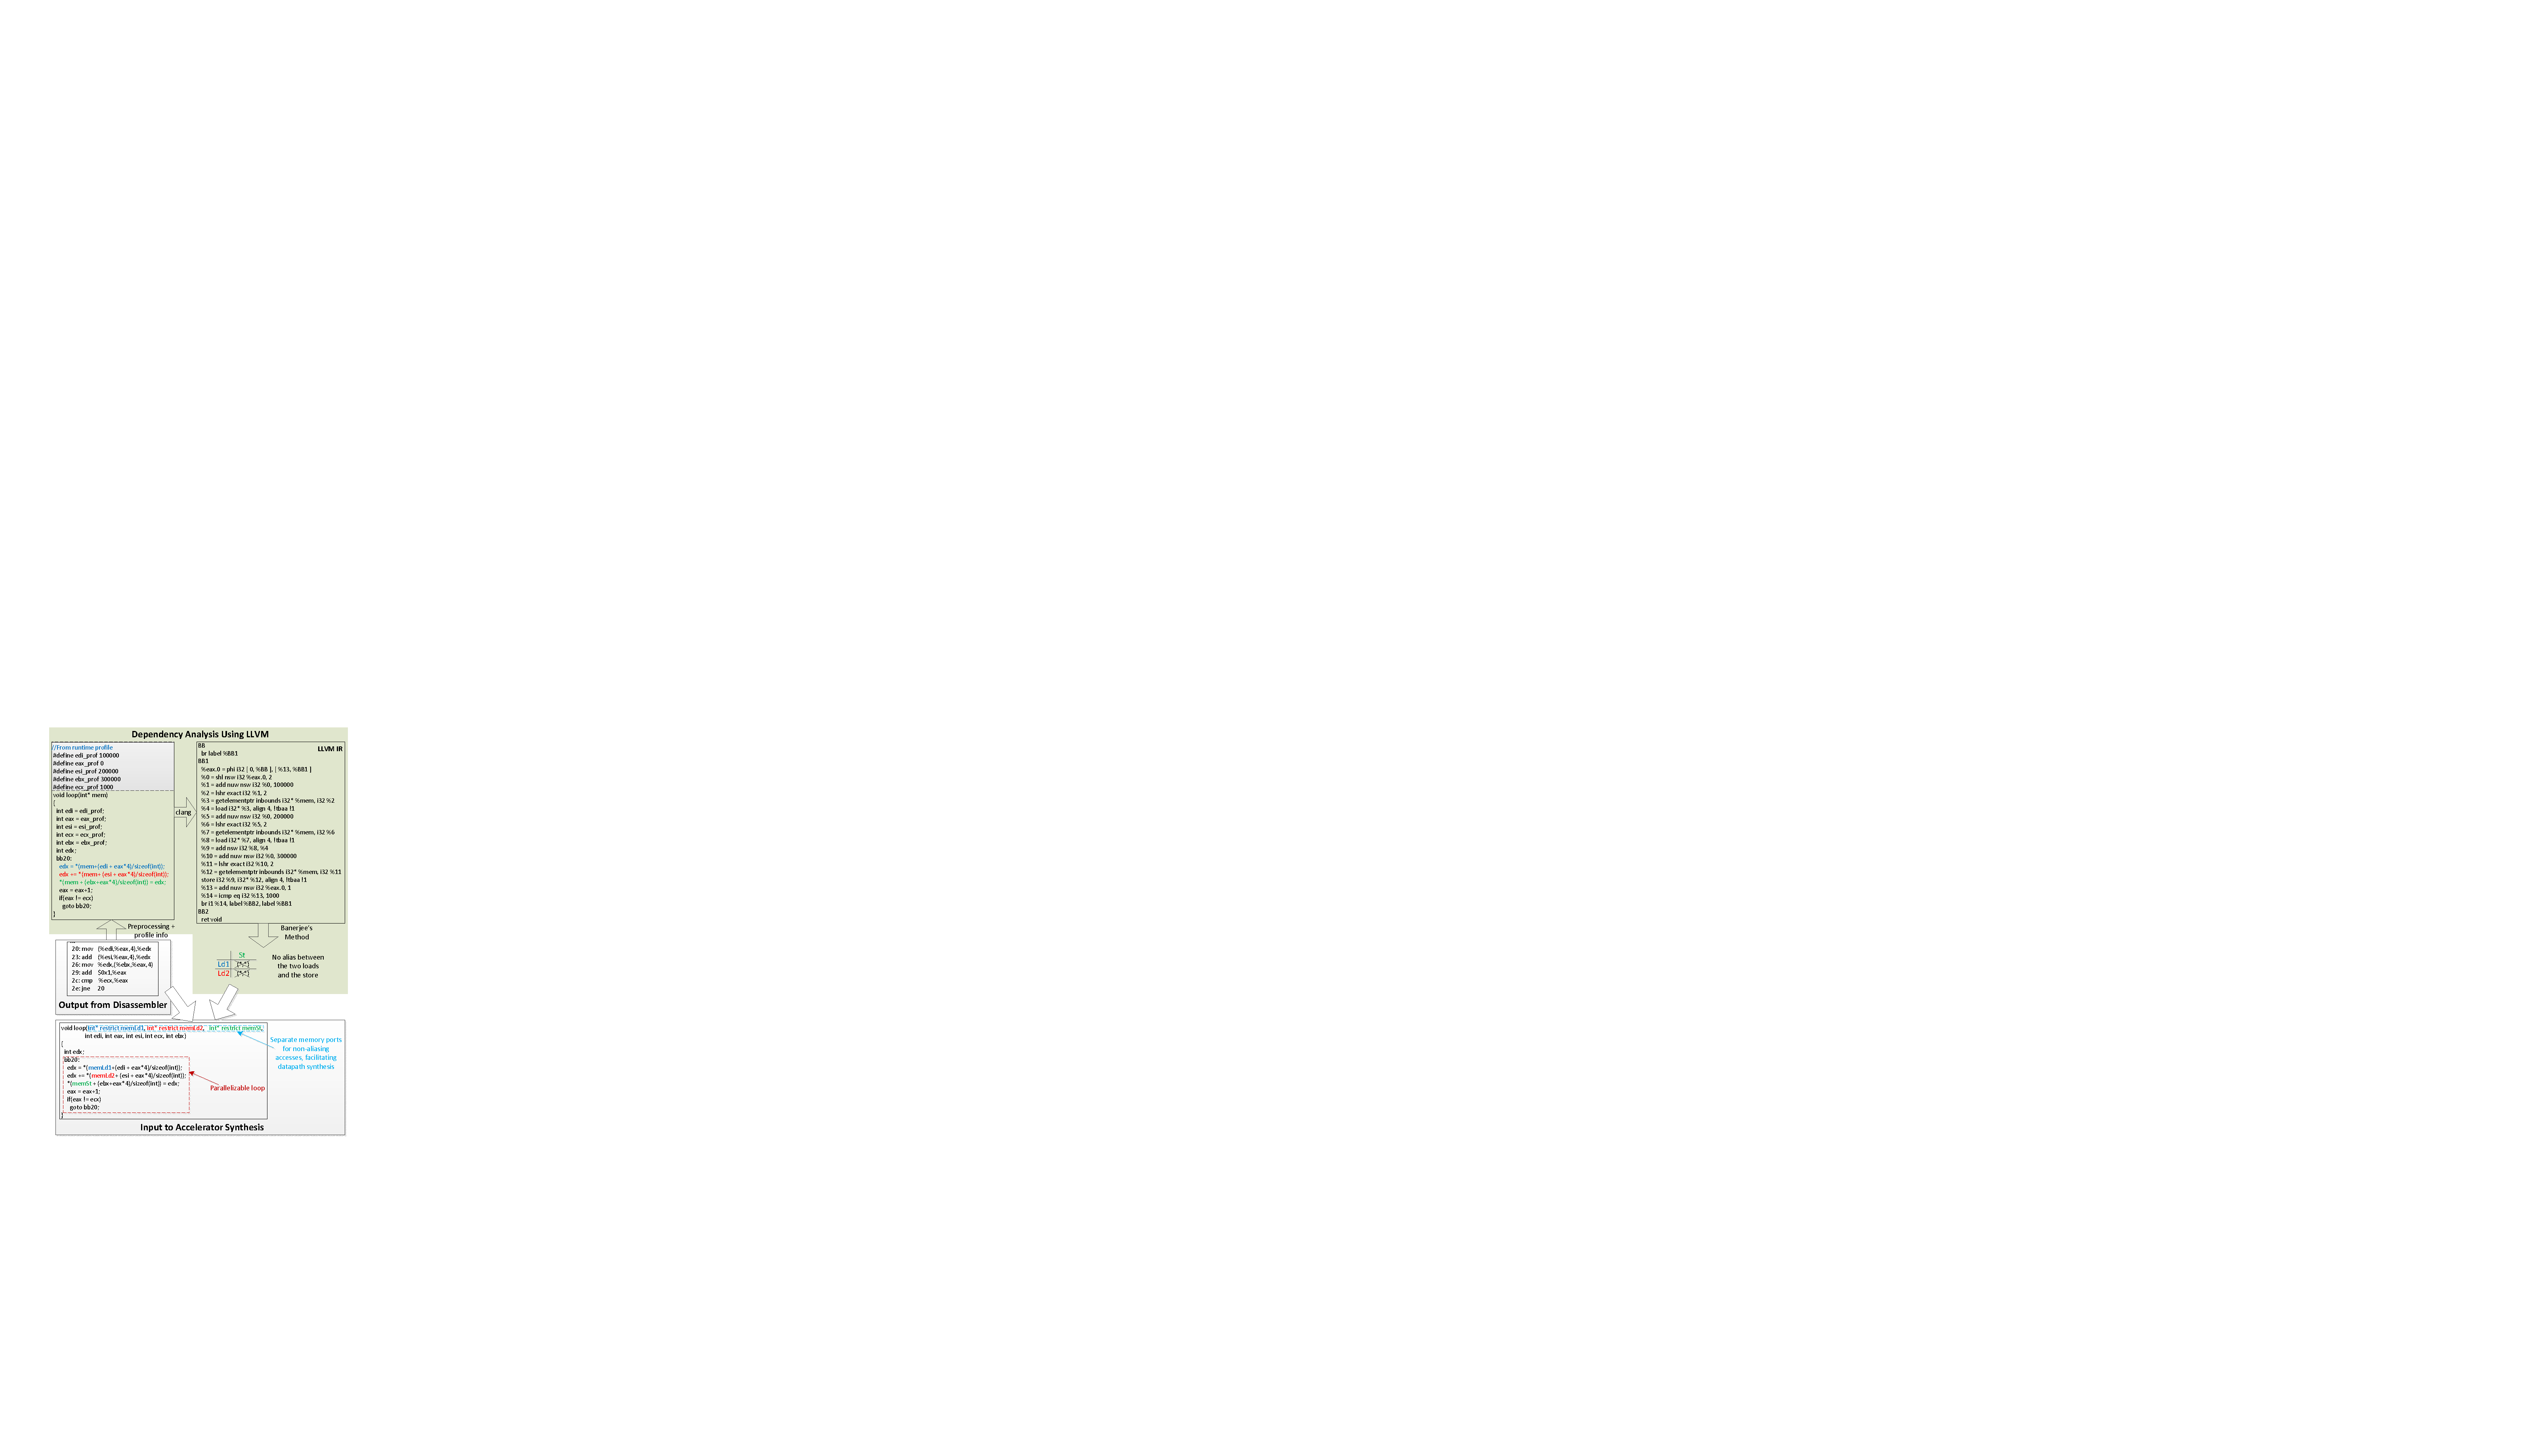
\includegraphics[width=0.87\linewidth]{chap6fig/analysisSteps.pdf}
\caption{From Disassembled Binary to Synthesizable C Code
\label{fig:mainSteps}}
\end{center}
\end{figure}


\subsection{Offline Phase: Accelerator Synthesis}

\subsubsection{Dependency Analysis}
To perform the offline dependency testing, we built an analysis pass within the LLVM framework. As LLVM takes C/C++ as input, a preprocessing step is performed
to convert the binary of the selected loops to C functions. It is also in this step when we extract coefficients for the Diophantine equation and bounds for loop indices from past execution profiles.
The numbers obtained are substituted as constants into the C functions, enabling the subsequent analysis. 
In the original binaries, these variables are often stored in the memory. 
Thus in addition to examining their past values, we also perform a check to ensure their memory locations do not alias with any other references performed by the loop nest, again using the addresses observed from the profile. This check can be easily formulated using Banerjee's method--we essentially have a set of affine
functions which only contain constant terms. Alternatively, these locations can often be
recognized as part of the call stack, and are normally completely disjoint from
the ``moving" part of the memory footprint in the loop. We can thus easily disambiguate them using a simple
range test. Of course, when the accelerator is actually being invoked, these tests would need to be run again, as will be described in later in this section.


 
Figure~\ref{fig:mainSteps} illustrates the steps involved in converting binary to a synthesizable C function. 
The original output from the disassembler is used to generate two
different versions of C functions. The first, incorporating values collected from past execution profile, can be analyzed by Banerjee's method. The results are the dependency direction vectors between memory operations. In this particular case, the store and load operations are found to be non-aliasing. This information is then used to generate the final C function, where each memory access is offset from a different pointer. Whether we
feed this version to conventional HLS or our pipeline generation flow, separate pointer
arguments can potentially be mapped to multiple memory ports, through which data requests can be initiated
independently.


%are applied to a loop doing simple vector addition.%example in figure~\ref{fig:mangledMem}.
\subsubsection{Memory Level Parallelism}
\label{subsec:mlp}
There are actually two levels of parallelization when it comes to scheduling memory accesses during HLS. As shown in figure~\ref{fig:mainSteps}, the absence of dependencies between memory operations allows for their association with
different pointers. The scheduling engine in the HLS tool can then schedule
them without being constrained by the original program order. However, multiple pointers may still be assigned to a single physical memory interface. The structural hazard would then constrain the action of the scheduler,
as a single memory port may only accommodate one load and one store per cycle.
To loosen this structural constraint, it is possible to create multiple memory
ports, each associated with a subset of pointer arguments. More aggressive scheduling, from the datapath's perspective, can then be performed. In addition, certain memory operation inside a loop can be converted to burst
access when it does not have to share the port with others. This frequently boost the efficiency of the off-chip bandwidth usage. In the decoupled computational pipelines described in chapter~\ref{decoupleChap}, as each separable memory access is  independently scheduled in a standalone module, which has its own memory port, both levels of memory parallelism are taken advantage of.
%This is illustrated in figure~\ref{fig:showInterfaceOccupancy}, which captures the occupancy of the interface between the FPGA accelerator and the memory subsystem in our experiment platform.

\begin{comment}
\begin{figure}[htp]
\begin{center}
\includegraphics[width=0.9\linewidth]{chap6fig/chipscope.pdf}
\caption{Two accelerators, one with memory level parallelism one doesn't, show chipscope 
\label{fig:showInterfaceOccupancy}}
\end{center}
\end{figure}
\end{comment}

The precondition for exploiting memory level parallelism is the non-overlap of addresses accessed by memory operations. This is especially true if they are to be issued through multiple ports, 
%they need to be completely independent from each other 
as we assume the RTL generation backend, the interconnect and memory subsystem may all be aggressively reordering these requests -- by inferring burst accesses or buffering.
Therefore, for every pair of accesses whose ordering matters (i.e. excluding load-load pair), we check the direction vector (*,*,...), and associate each access to a separate
pointer if the test result is negative. In section~\ref{subsec:pmd}, we described how memory barriers are inserted to prevent overly conservative dependency annotation.
Similarly, in our binary based flow, if memory dependencies are carried by outer loops,
memory barriers can also be inserted to facilitate the partitioning of memory access interfaces. The direction vector to test here is  (=,=,..,*,*),
where "=" occupies all levels including and outside of the level of insertion. If negative results is produced, we can be certain that within the same iteration of the loop where the barrier is inserted, the pair of tested instructions do not reference the same addresses.
Therefore any reordering of memory operations will be valid. An example of this is shown in figure~\ref{fig:withOrWithoutBarrier}. 


\begin{figure}[htp]
\begin{center}
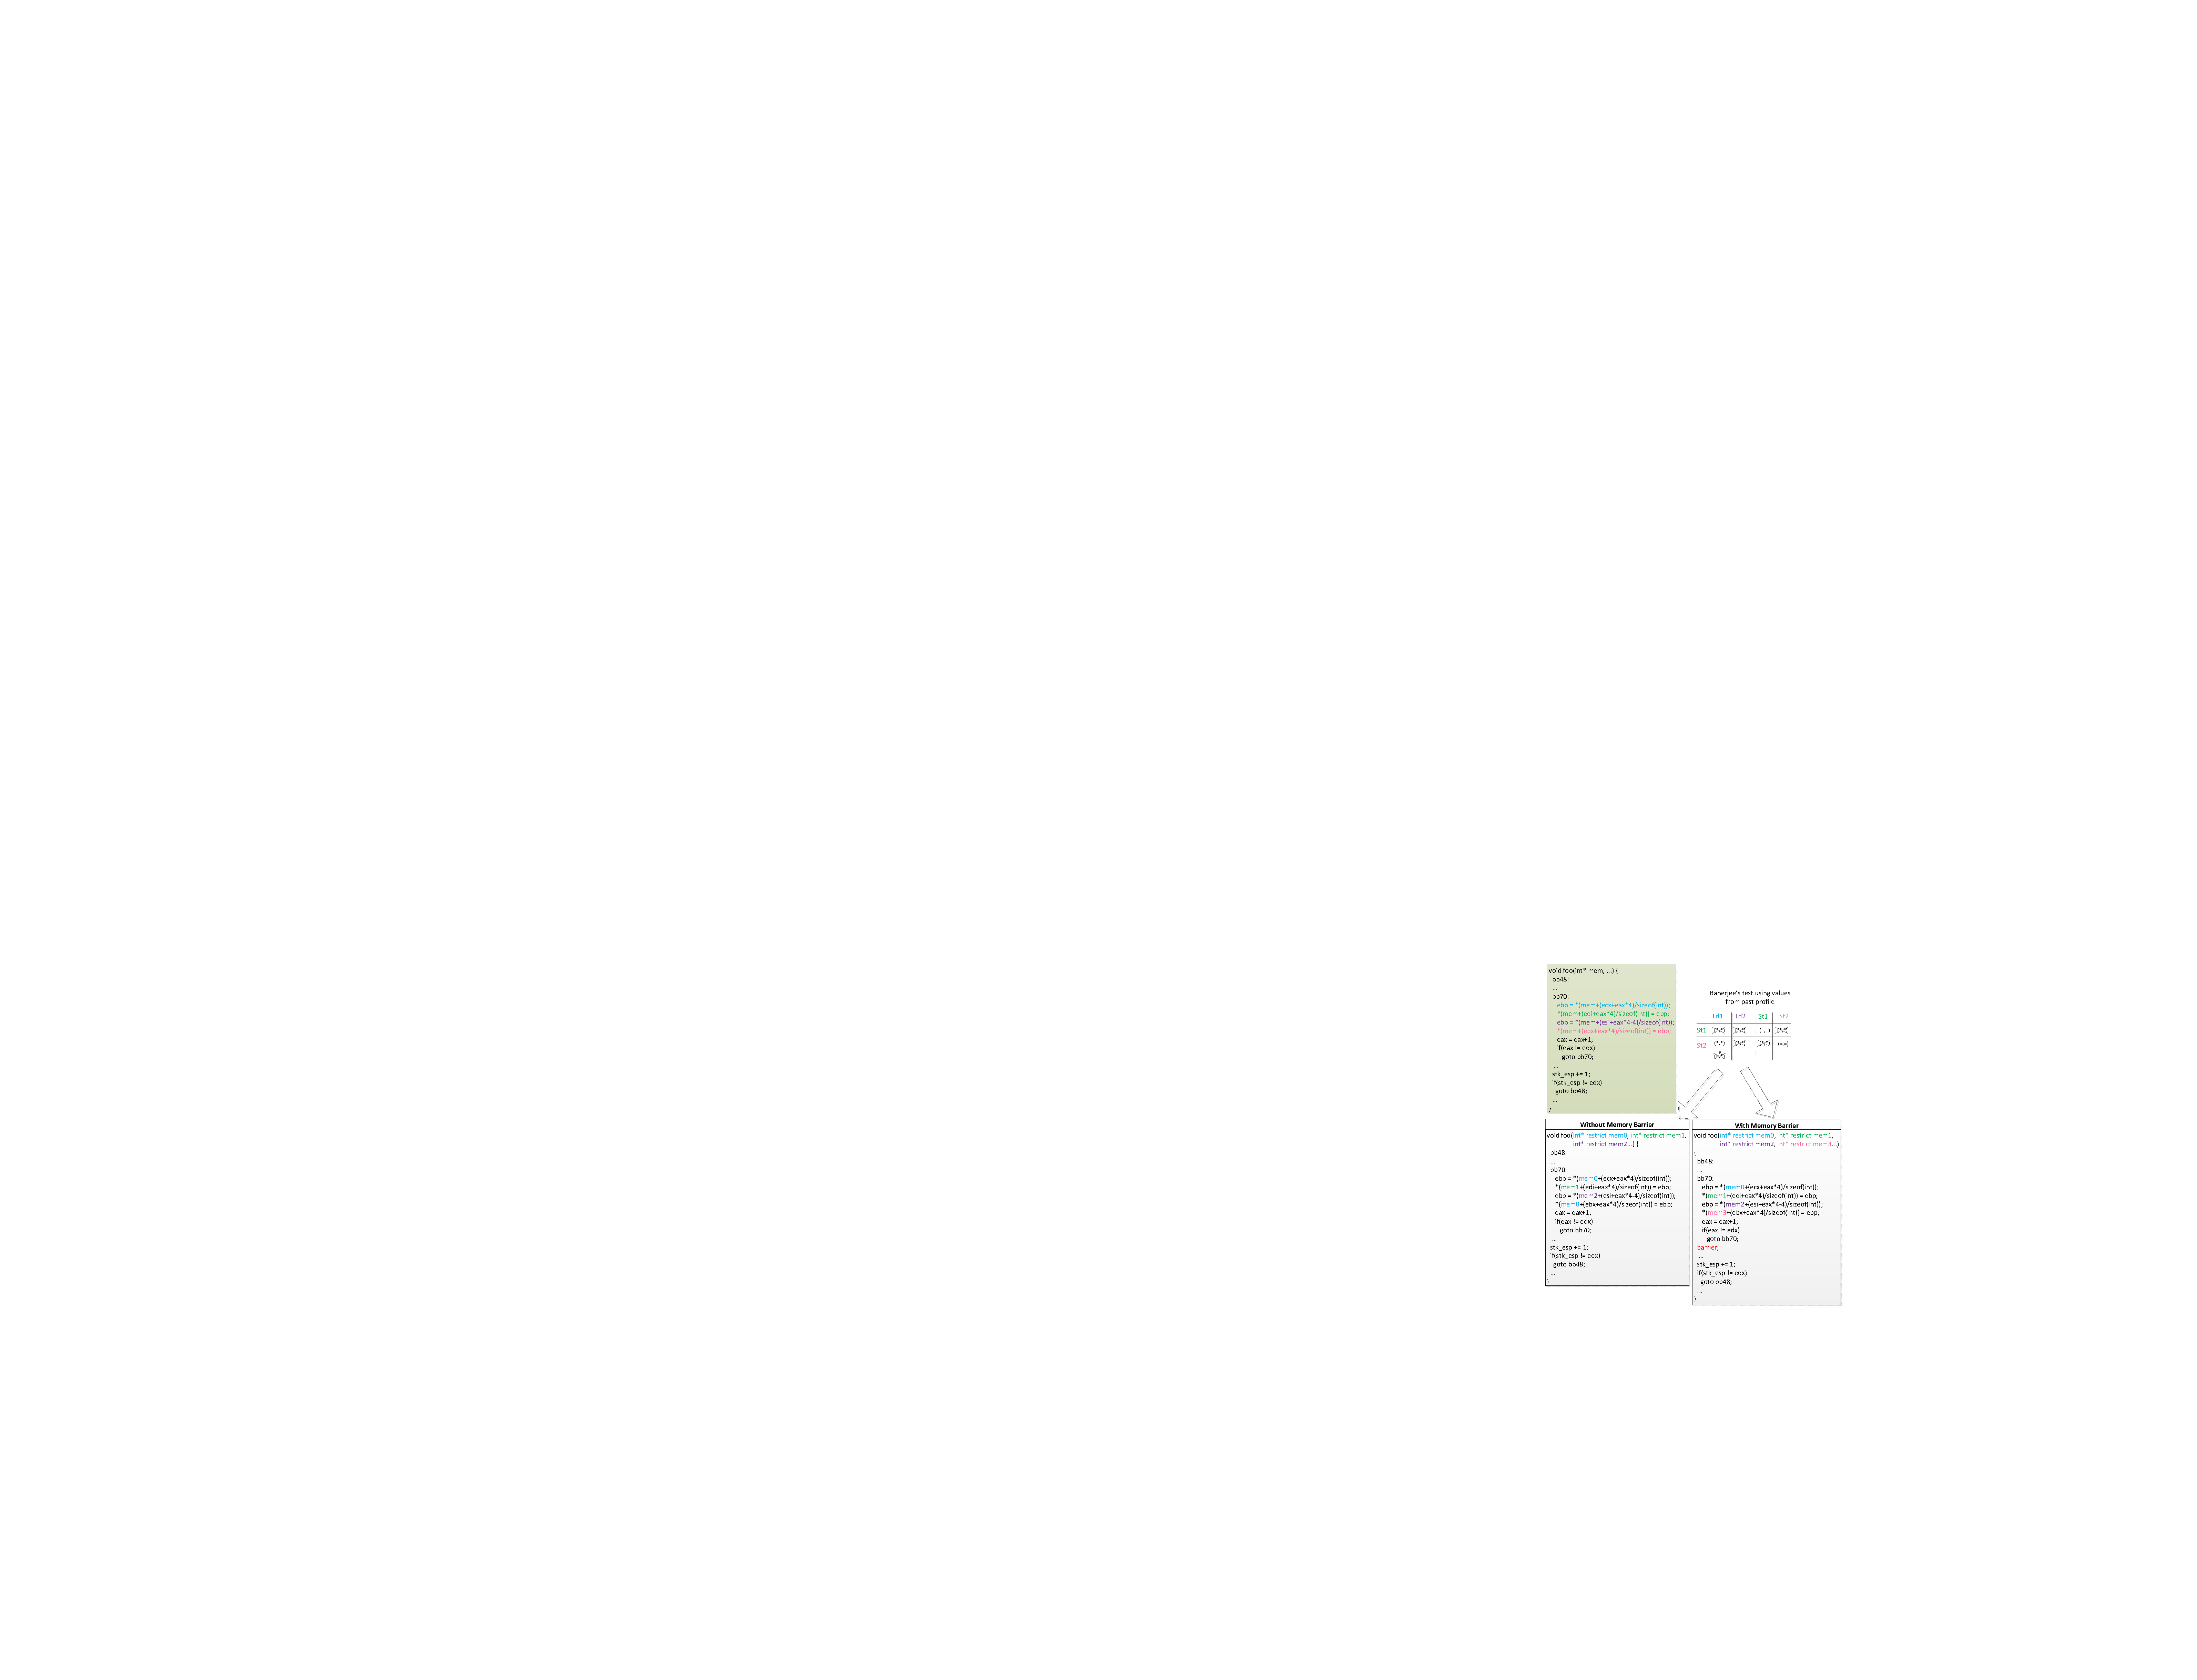
\includegraphics[width=0.9\linewidth]{chap6fig/memOrMemBarrier2.pdf}
\caption{Partitioning of Memory Access Interface with Insertion of Memory Barriers 
\label{fig:withOrWithoutBarrier}}
\end{center}
\end{figure}


\subsubsection{Coarse Grained Parallelism}
\label{subsec:cgp}

In addition to memory level parallelism, the loop shown in the example also has coarse grained parallelism between iterations of the inner loop. A typical high level synthesis flow can employ several common mechanisms to parallelize loops, as illustrated in figure~\ref{fig:fpgaparal}. 
For the inner most
loop, it is generally very cost effective to pipeline the loop, starting a new iteration before the previous one finishes. If
the iterations are parallelizable, the initiation interval would be 1.
Assuming there are $M$ iterations, the total execution time of the loop
would roughly be $M$ cycles (not counting stalls introduced by cache misses). To further reduce this number, loop unrolling
can be performed. It combines multiple iterations into one, effectively
turning inter-iteration parallelism into fine grained parallelism. 
The iteration count is reduced by the unroll factor ($U$) while the II does not change. Consequently, the total execution time is reduced to roughly $M/U$ cycles with a approximately $U$ fold increase in area. 

\begin{figure}[htp]
\begin{center}
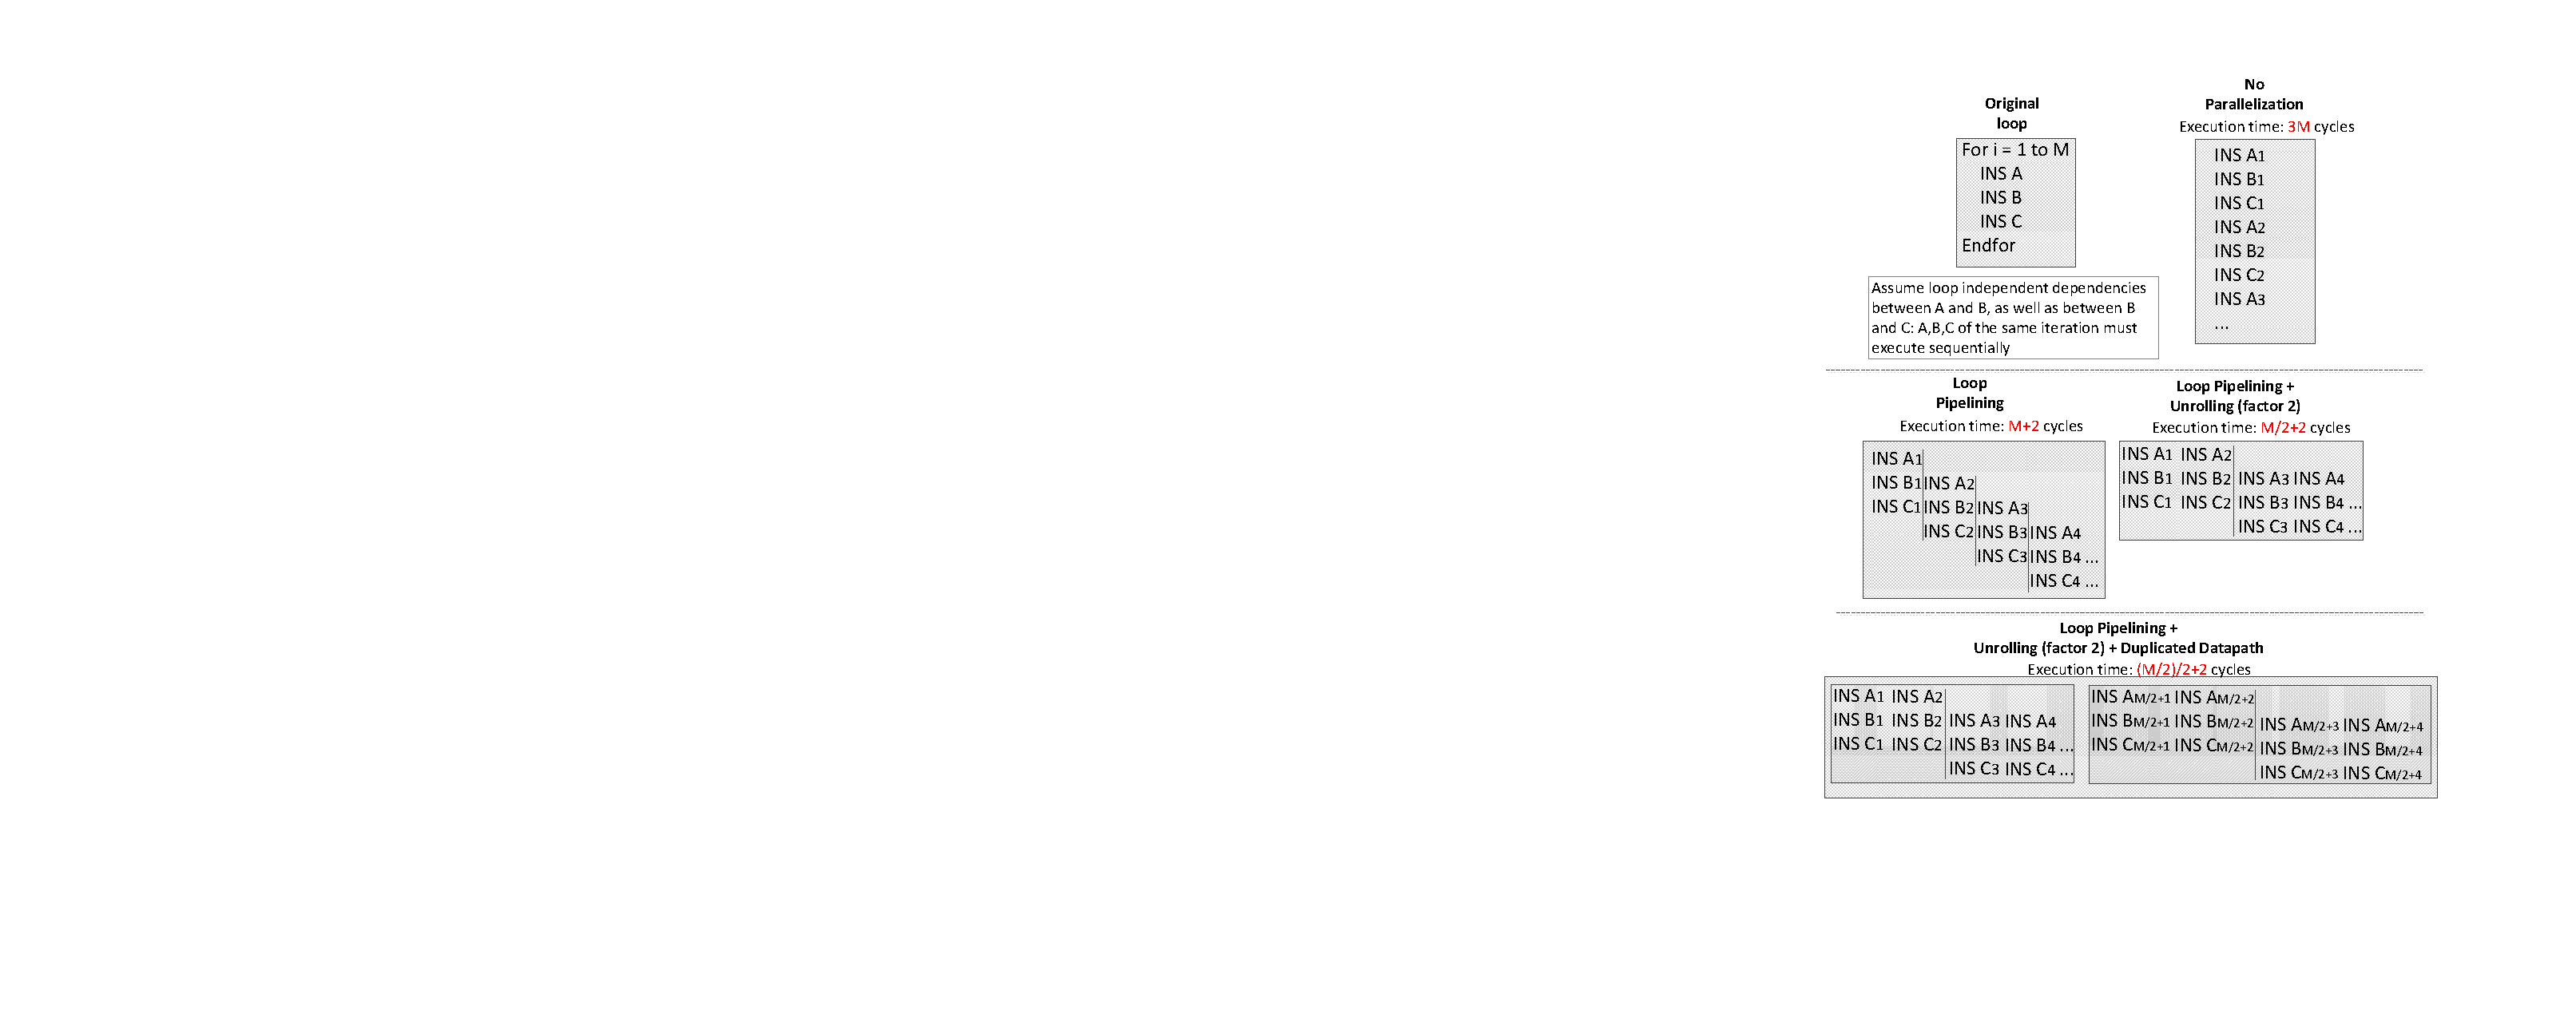
\includegraphics[width=0.8\linewidth]{chap6fig/fpgaParallel.pdf}
\caption{Parallelization in FPGA Accelerators
\label{fig:fpgaparal}}
\end{center}
\end{figure}

To improve the throughput of the accelerator even further, multiple
independent datapaths can be instantiated, each performing a subset of 
the iterations. This technique can be used to parallelize outer loops
as well. For loop with a large number of iterations, this technique provides a good way to trade off more on-chip resources for better performance, although
it also incurs some extra synchronization overheads. Another advantage of
having multiple datapaths is the independence between their controllers.
In an earlier chapter(section~\ref{motex}), we illustrated the vulnerability
of a single monolithic schedule to data access latencies and the resulted
underutilization of the memory bandwidth. In the presence of coarse grained parallelism, it is much easier to fully exploit the data bandwidth provided
by the platform, as each datapath independently generates requests, whether
its peers are stalled or not. 
Certain platforms also provide multiple channels
for off-chip memory access, which can be more easily utilized with duplicated datapaths. 


%Figure~\ref{fig:fpgaparal} illustrates the described parallelization schemes for FPGA accelerators.
\begin{comment}

\begin{figure}[htp]
\begin{center}
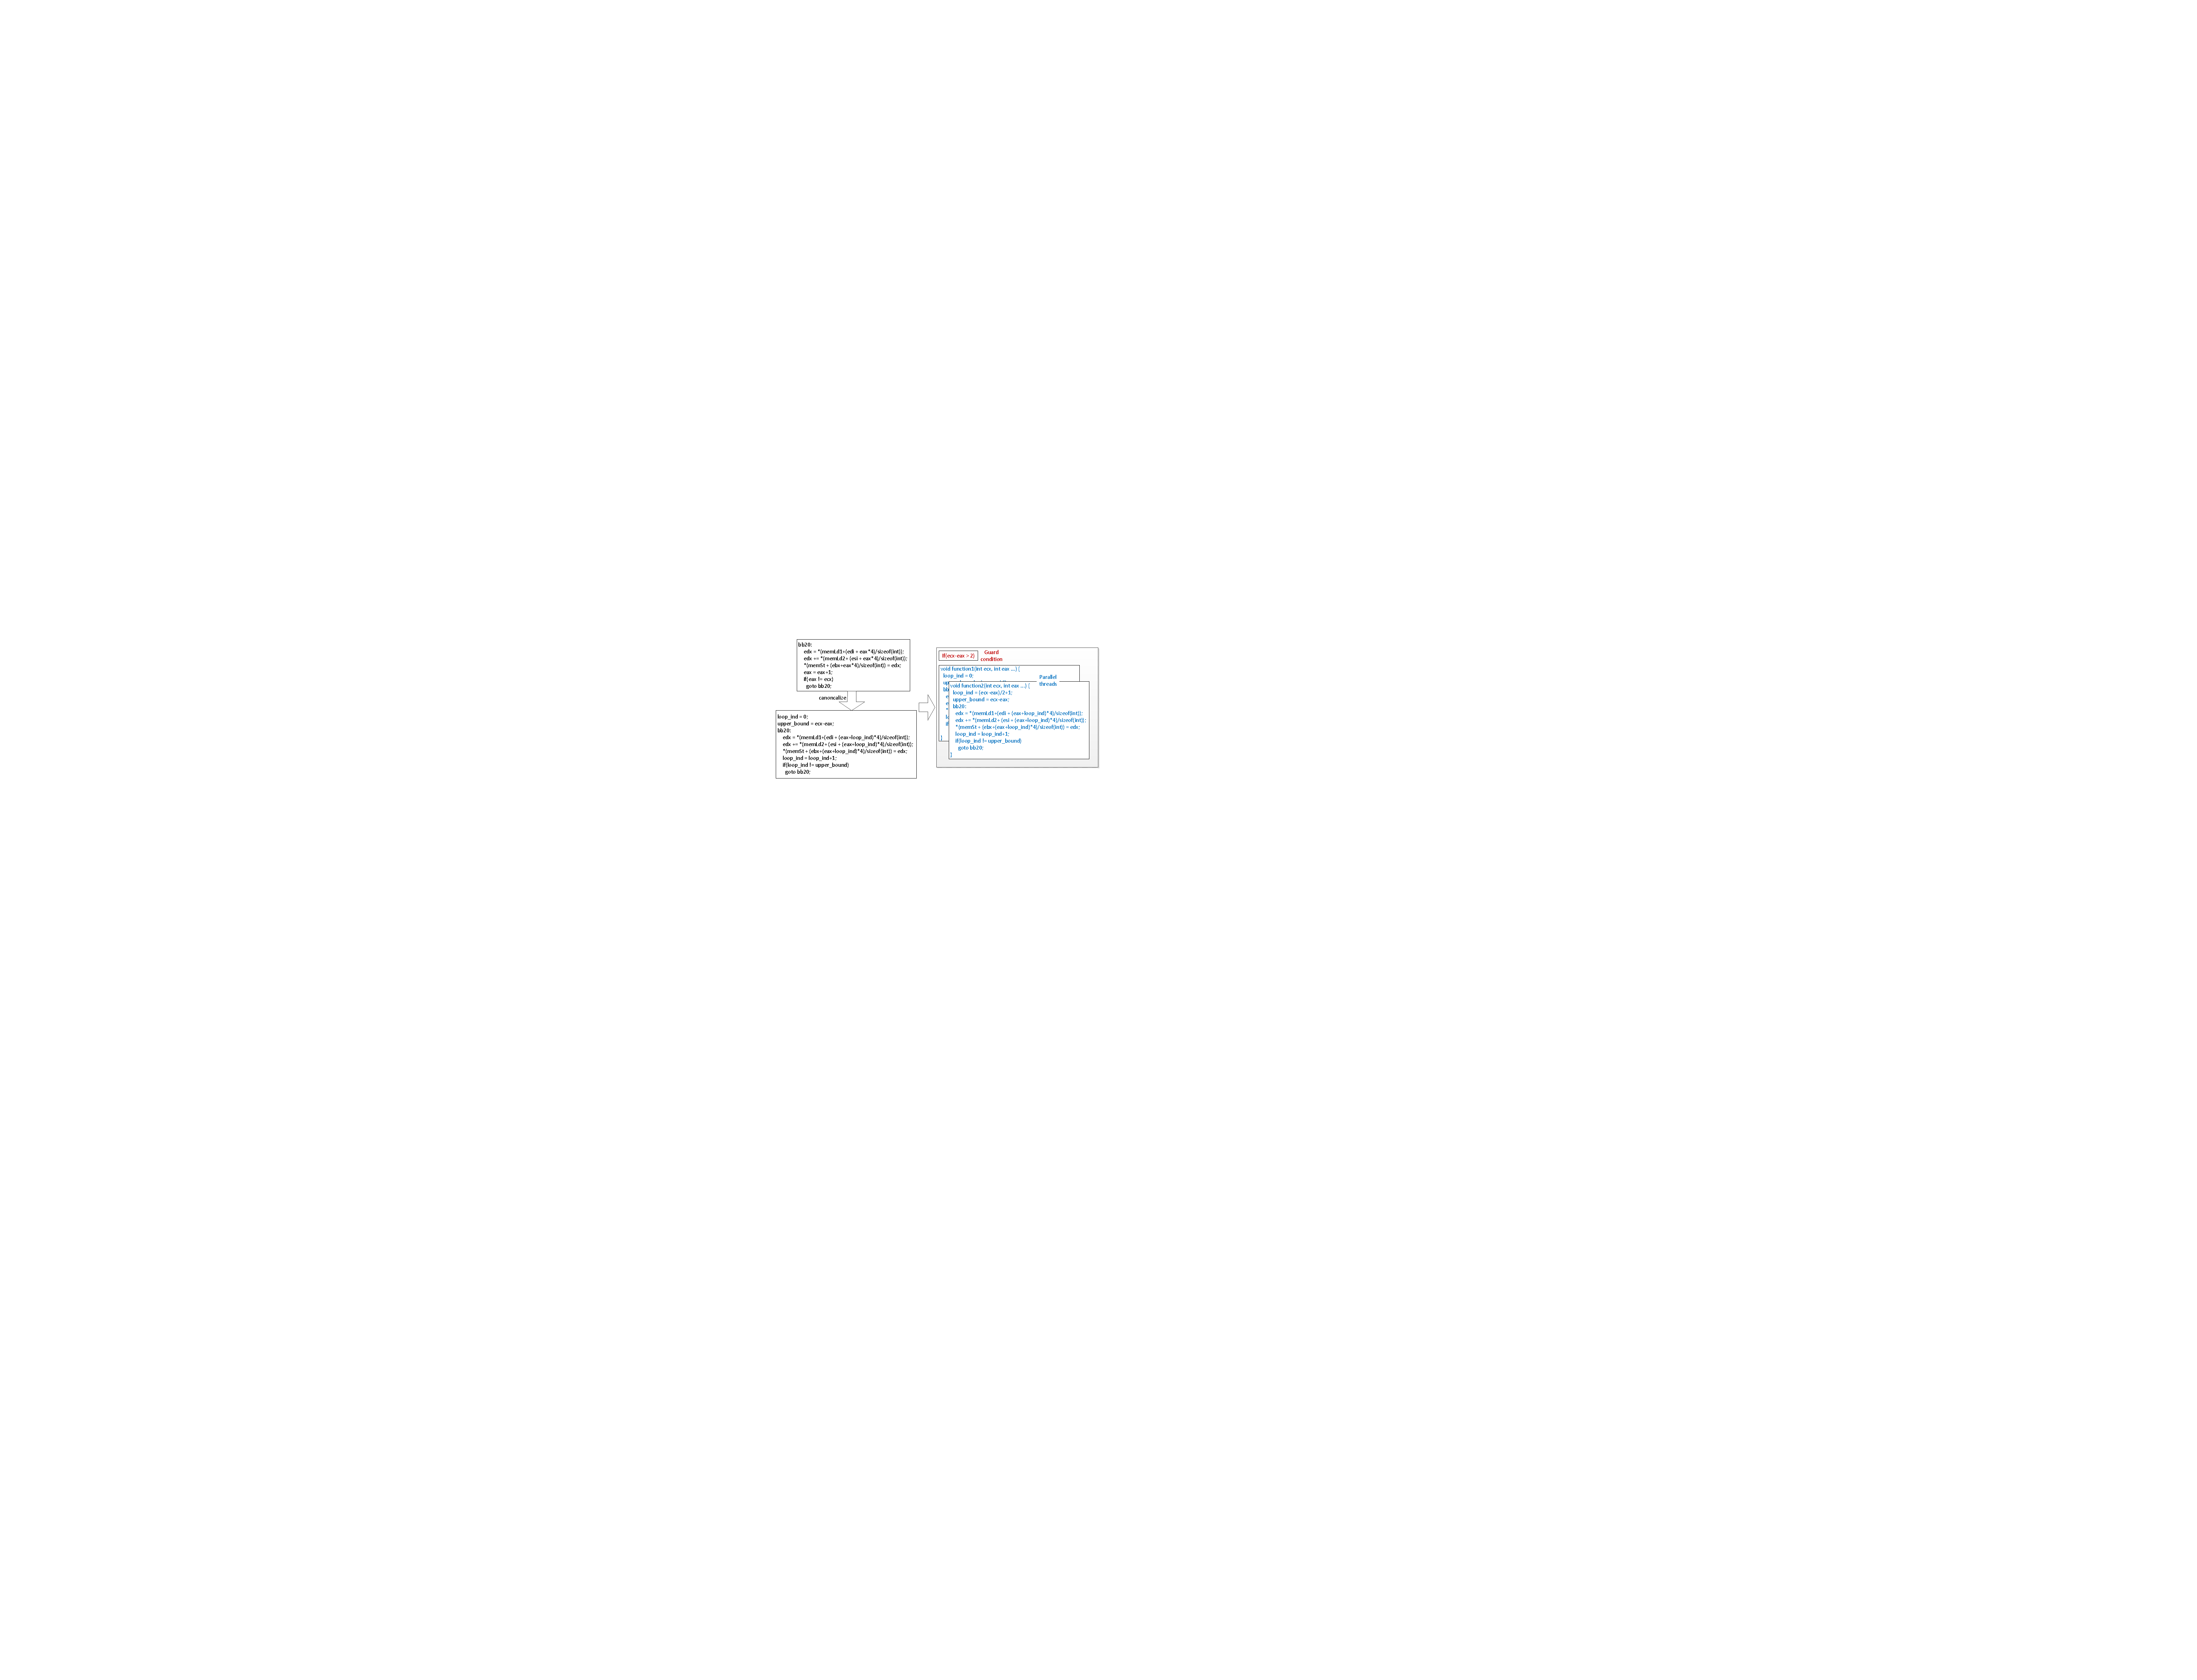
\includegraphics[width=1.1\linewidth]{chap6fig/threadSplit2.pdf}
\caption{Thread-level Parallelization 
\label{fig:threadP}}
\end{center}
\end{figure}
\end{comment}

\begin{figure}[htp]
\begin{center}
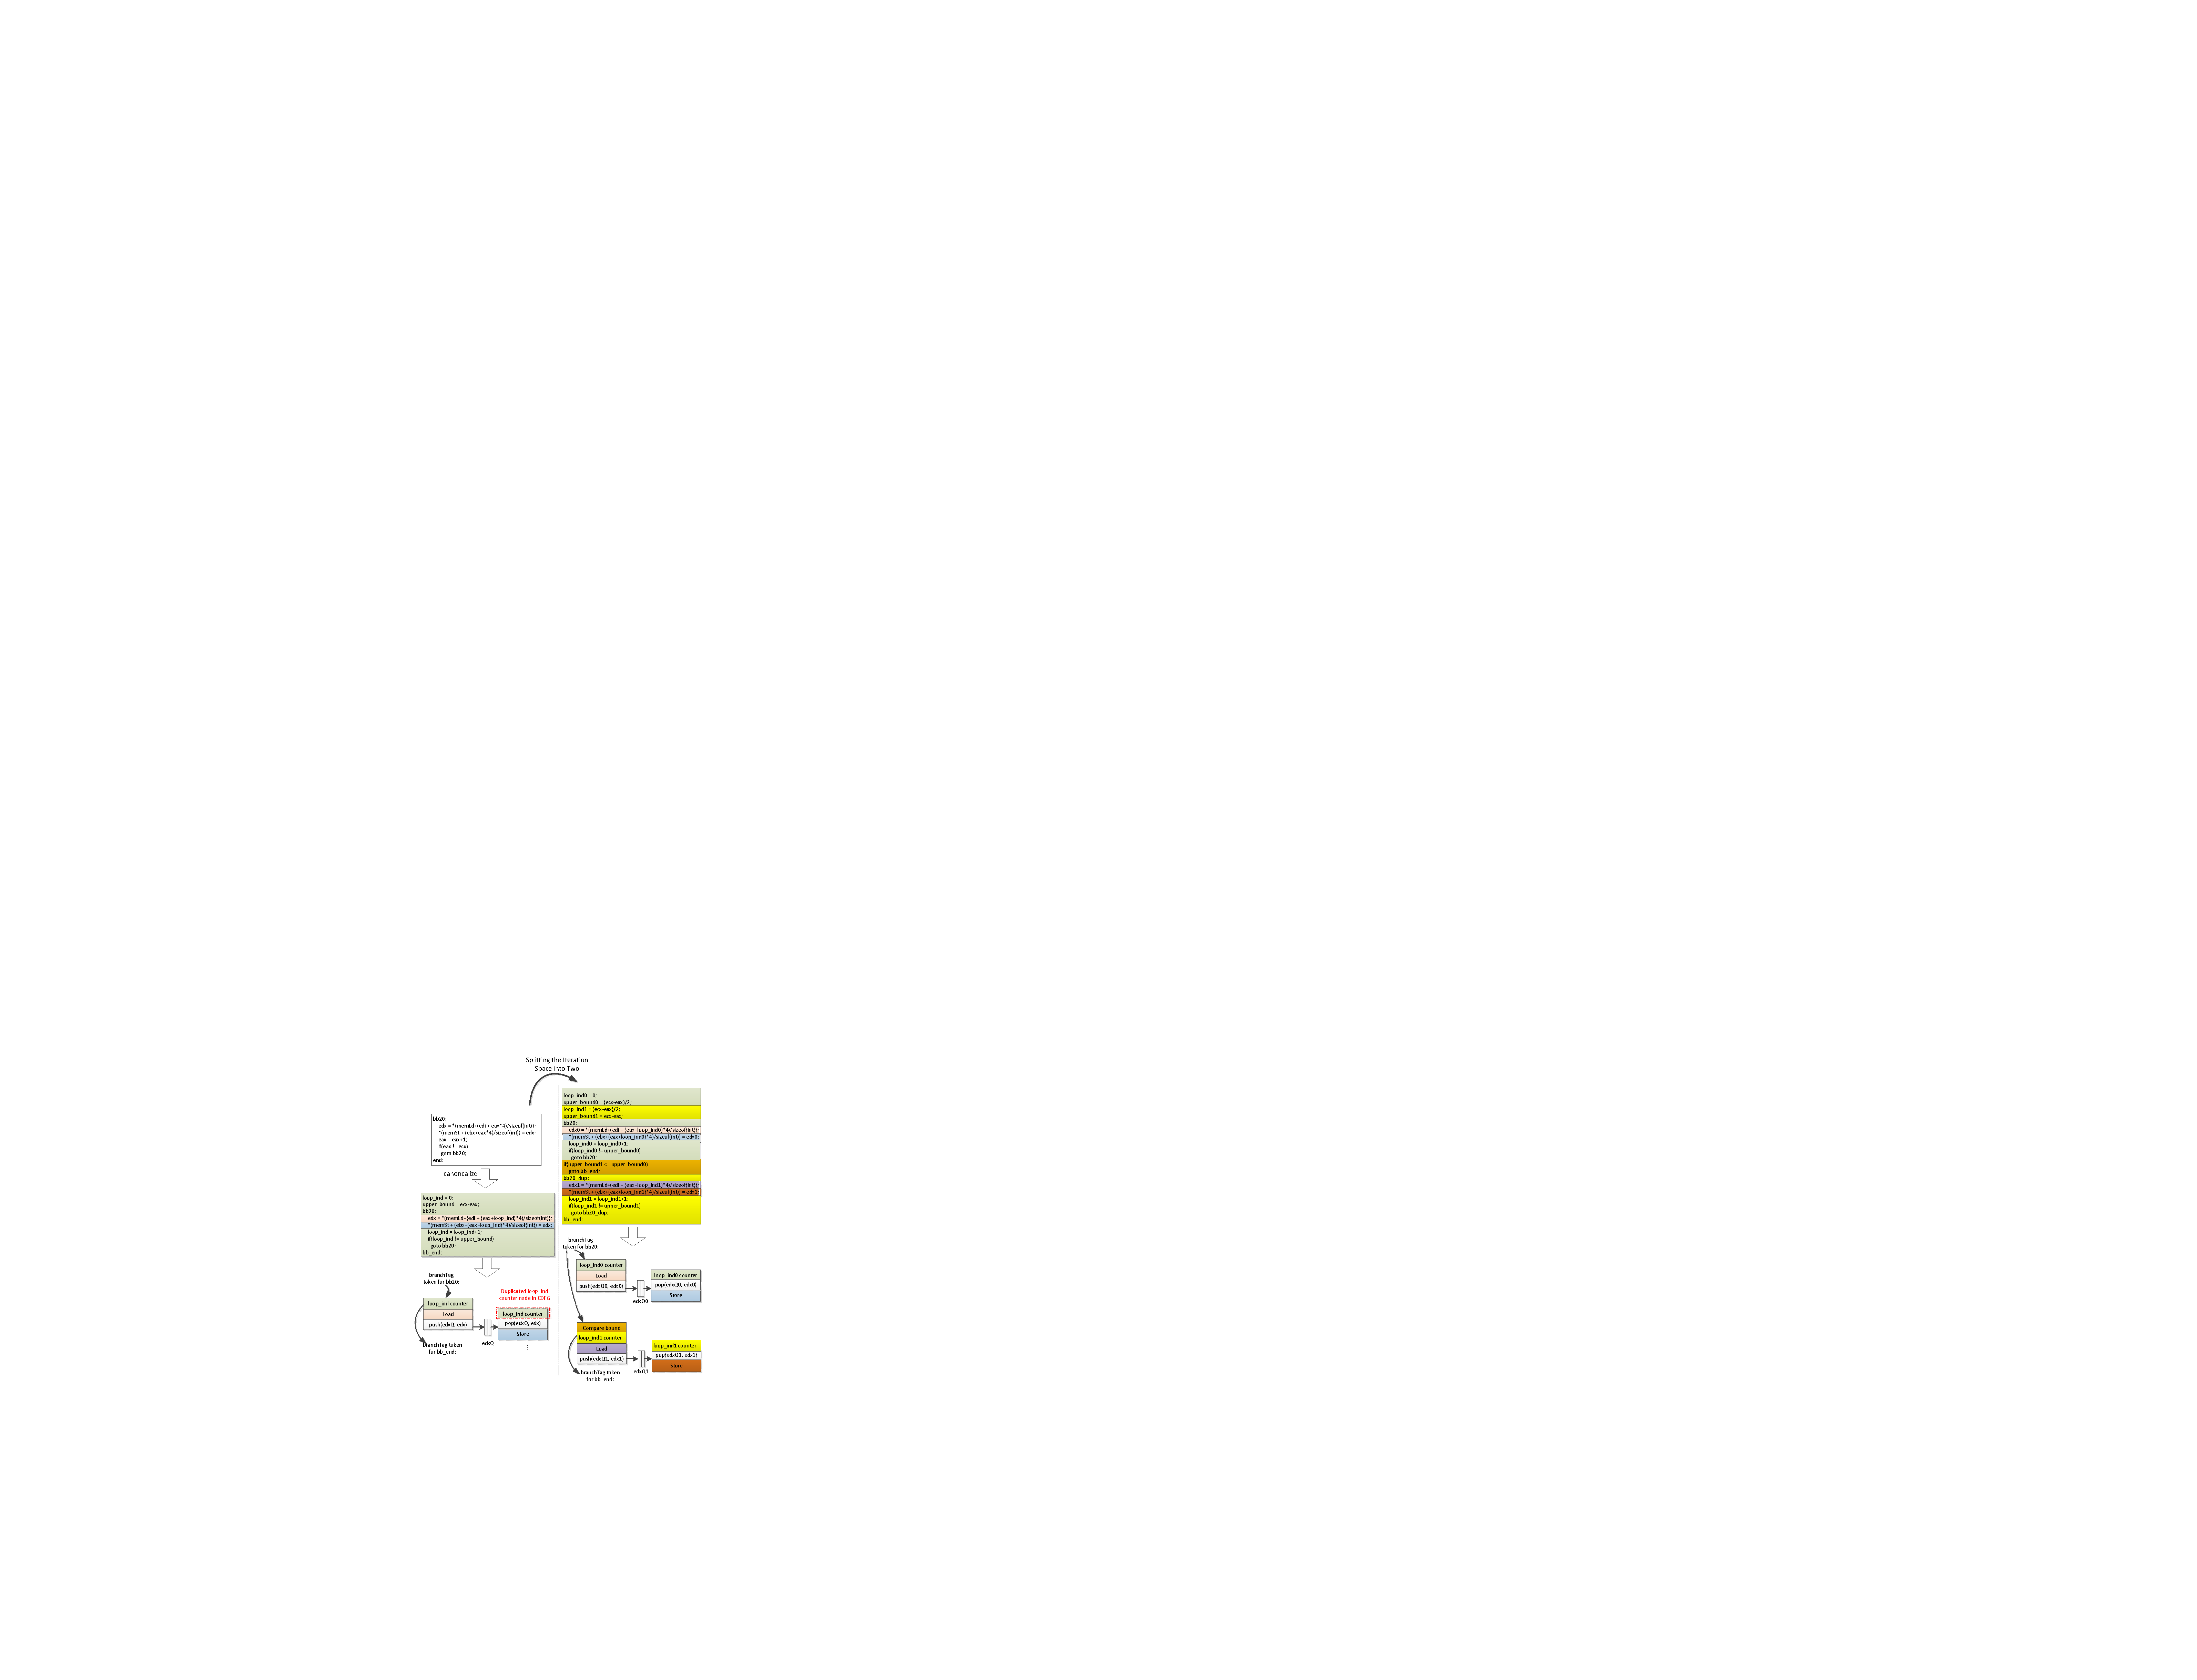
\includegraphics[width=1.0\linewidth]{chap6fig/naturalSplit2.pdf}
\caption{Thread-level Parallelization 
\label{fig:threadP}}
\end{center}
\end{figure}


We can draw similarities between these techniques and the compiler optimizations targeting architectural features
of various parallel processors. Loop pipelining was a scheduling technique
widely used for VLIW machines, where it is often called software pipelining. Loop unrolling, in the synthesis of FPGA
accelerators, is similar to vectorization, as a wider processing engine
is now used to process multiple iterations simultaneously. The replication of
datapath is essentially generating multithreaded implementation from a serial specification. 
Previous research in automatic parallelization can thus be
leveraged for our flow. In this work, we are not trying to invent new techniques, but to enable past work to be applied to program binaries on FPGA platform. In fact, techniques like loop unrolling and loop pipelining are already built into commercial HLS tools, and can be easily applied using directives.


To generate multiple parallel and independent datapaths, one approach is to convert a single loop nest to multiple functions.
Each function can be easily synthesized into an independent accelerator, but synchronization mechanisms might need to be explicitly inserted so that outer level loop and the container function can correctly manage accelerators running in parallel~\cite{Sheffield:EECS-2013-185}. 
For our flow however, as we are using the decouple computational pipeline as the architecture template, a simple splitting of the iteration space can naturally lead to the generation of parallel processing pipelines, with proper synchronization achieved by the sending and receiving of tokens. Figure~\ref{fig:threadP} illustrate how this process is achieved using a simple example. Even though we constructs a control flow where the two parts of the iteration space resulted from the split are executed sequentially, due to the optimizations built into the pipeline generation flow, two parallel pipeline branches are created. Note the second half of the loop nest ($bb20\_dup$) is predicated by the same branch going into the first due to the aggressive predication described in section~\ref{subsec:cde}. Consequently, instead of being activated after the completion of loop $bb20$, it executes in parallel to it. Of course, if there are actual dependencies between these two halves of the loop, the pipeline branch running $bb20\_dup$ will be stalled waiting for the result from $bb20$. The overall execution would then be practically serialized. Also, the loop counters, which are relatively cheap, get duplicated to multiple stages in the computational pipeline, but only one generates the branch token to be consumed by subsequent pipeline stages. This, along with any other data tokens the successor basic blocks need to read, collectively synchronize the completion of the loop nest with all its dependent operations. 
 
For conventional high level synthesis, it's often desirable to have thread-level auto-parallelization at the outer level of the loops. An architectural template is used in~\cite{Sheffield:EECS-2013-185} to accommodate and explicitly coordinate multiple independent accelerators
each with its own FSM controller. The synthesis of the accelerators and the instantiation of the top level management circuitry are two separate processes and to perform inner loop thread level parallelization would be rather intrusive. There are also cases where threads are manually programmed into the application  
%the users would have explicitly specified the points of synchronization using primitives in 
using APIs such as OpenMP/Pthread. Since the users have explicitly specified the points and mechanisms of synchronization, the tool can 
leverage a prebuilt library of software/hardware to implement these primitives, managing multiple datapaths running simultaneously. In~\cite{legupmultithread} for instance, each independent thread the user created is mapped to a separate datapath with its own controller, and a software wrapper is synthesized to manage it in the software domain at the top level. Meanwhile, OpenMP pragmas, when attached to the inner loops, direct the HLS tool to create parallel internal accelerators.
The FSM managing the container thread would block until all the internal accelerators finish executing.  
%the HLS tool may create a software wrapper for each independent thread~\cite{legupmultithread}, who would then be managed in the software domain. 
%Note in~\cite{legupmultithread}, openMP threads in the inner loop can be synthesized into parallel datapaths. However, without having independent controller state machines, these datapaths are, in essence, synchronizing with each other every clock cycle. This operation mode eliminates some of the benefits of having thread parallelism.
Our flow, on the other hand, does not have any noticeable difference in the implementation of outer and inner loop parallel threads. 
As the pipeline generated is controlled in a highly distributed way, making independent inner loop (or outer loop) thread only requires a  loop splitting which can be easily performed to the intermediate representation. A unified framework involving only source to source transformation can therefore be applied to all levels in the loop nests.  


%The synchronization with successor basic blocks, who are predicated on the completion of the loop, is therefore achieved.

\begin{comment}
For thread level parallelization, LLVM can again be used to create multiple functions from a single loop nest. As illustrated in figure~\ref{fig:threadP}, the parallelizable dimension of the iteration space
is to be split evenly, a guard condition is also generated to ensure the validity 
of the derived bounds for all the threads. 
Each thread, encapuslated by a function, corresponds to a chunk of the loop iterations and runs in parallel with its peers.
\end{comment}




For the target applications of our flow, the memory footprint of the computation is assumed to be
much larger than the capacity of on-chip RAM. With the fetching of data
from off-chip storage being a major task of the generated accelerators,
thread-level parallelization is often preferred to loop unrolling.
Unrolled 
%inner 
loops usually contain multiple memory accesses which were
initially folded as one operation. In cases where the referenced addresses are contiguous, the original memory access can be converted to burst mode load or store, significantly improving the efficiency of memory bandwidth usage. Loop unrolling prevents this burst
inference from occurring as the original single stream of addresses is now broken
into two interleaved streams. 
On the other hand, in terms of the effort needed to perform loop unrolling v.s. generate multiple hardware threads, most existing HLS flows can easily perform the former when the user insert the appropriate directives, while thread creation and management, if being supported at all, may require code rewriting/refactoring. As mentioned in the earlier paragraph, the special mechanisms used to accommodate and synchronize multiple independent datapaths can also incur extra area overhead. Fortunately for our flow, the disadvantages in programming effort and resource usage for multithreaded hardware do not manifest themselves, as explained earlier. We can therefore focus on optimizing for the throughput of the final implementation. 



 %Of course, in applications where the overall speed is bounded by the compute throughput, this difference does not manifest itself.



%Loop unrolling makes more sense when the on-chip storage is partitioned into small scratchpad memories which can be accessed by the datapath simultaneously.
%Given the regularity of the targeted kernel, it is certainly possible to create a mechanism through which off-chip data gets prefetched and distributed into many distributed on-chip RAM. However, for the benchmarks where off-chip communication 
%is the main performance bottleneck, there is little benefit in doing this. 
%Also, the overhead of multiple datapath is only marginally higher than unrolled
%loop as the main overhead is only the extra control state machine.  













\begin{comment}

The actual implementation of the parallelization engine is built
on top of the LLVM framework. As LLVM takes C/C++ as input, we created a preprocessing step
to convert the binary of the selected loops to C functions.
It is also in this step when we extract
coefficients for the Diophantine equation and bounds for loop indices from past runtime profiles.
The numbers obtained are substituted as constants into the C functions, enabling the subsequent analysis. 
In the original binaries, these variables are often stored in the memory. 
Thus in addition to examining their past values, we also perform a check to ensure their memory
locations do not alias with any other references performed by the loop nest, again using the
addresses observed from the profile. 
Most of the time, these locations can be
recognized as part of the call stack, and are normally completely disjoint from
the memory footprint of the actual loop. We can thus easily disambiguate them using a simple
range test. Of course, when the accelerator is actually being invoked, this test would need to be
run again, as will be detailed in section~\ref{onlinephase}.


FIXME:There are many existing compiler passes within LLVM which facilitates the analysis ....
After the transformations, the LLVM IR is converted back to C, before HLS is used
to generate the final circuits. Multiple independent C functions can be generated
when multiple datapaths are desired in the final implementation. Vendor specific
pragmas are also inserted to provide guidance for the HLS tool. An example output,
which targets Vivado HLS backend, is shown in figure~\ref{}. 
\end{comment}



So far the analysis and parallelization are all performed independent of the actual
RTL generation. In essence we have devised a set of transformations applicable within the LLVM framework. A piece of disassembled binary is converted to C code, which is ready to be synthesized into the decoupled computational pipeline through the RTL generation backend. The last part of the \textit{offline phase} involves pushing the RTL through traditional FPGA CAD flow. This step can take between tens of minutes to a few hours,
depending on the size of the design and the utilization of the FPGA chip. 

%In this work, however, we aim to 

%In addition, as the hardware on FPGAs can be parameterized on a per application basis, there is a huge design space where the high level input
%for HLS as well as the supporting infrastructure (e.g. on chip buffer) can
%be co-tuned. A thorough exploration of this space is left to future work.

%are affine expression of the loop indices, each with a different coefficient,
%The range of memory
%locations accessed by each load/store instructions under each loop level
%is used as a rough approximation of locality. To make the comparison fair, this
%range is also divided by the number of iterations in the corresponding levels.





\subsection{Online Phase: Parallelism Validity Check and Accelerator Execution}
\label{onlinephase}
\begin{comment}
When applying Banerjee's method, a particular direction vector $\vec{v}$ is subjected to test, and the result reveals if a pair of memory accesses are dependent in $\vec{v}$'s direction. 
%first used as the constraint and the result of the test reports if this vector may hold true for a pair of memory accesses. 
%Therefore, 
To find all the direction vectors for dependencies, a hierarchy
of tests are therefore involved. For a pair of memory accesses in a two level loop nest, the possible tests are shown in figure~\ref{fig:testingHier}, where ``$\ast$" denotes a union of ``$<$", ``=" and ``$>$". Negative test result from any node in the hierarchy eliminates the necessity to continue testing its subnodes.  


\begin{figure}[htp]
\begin{center}
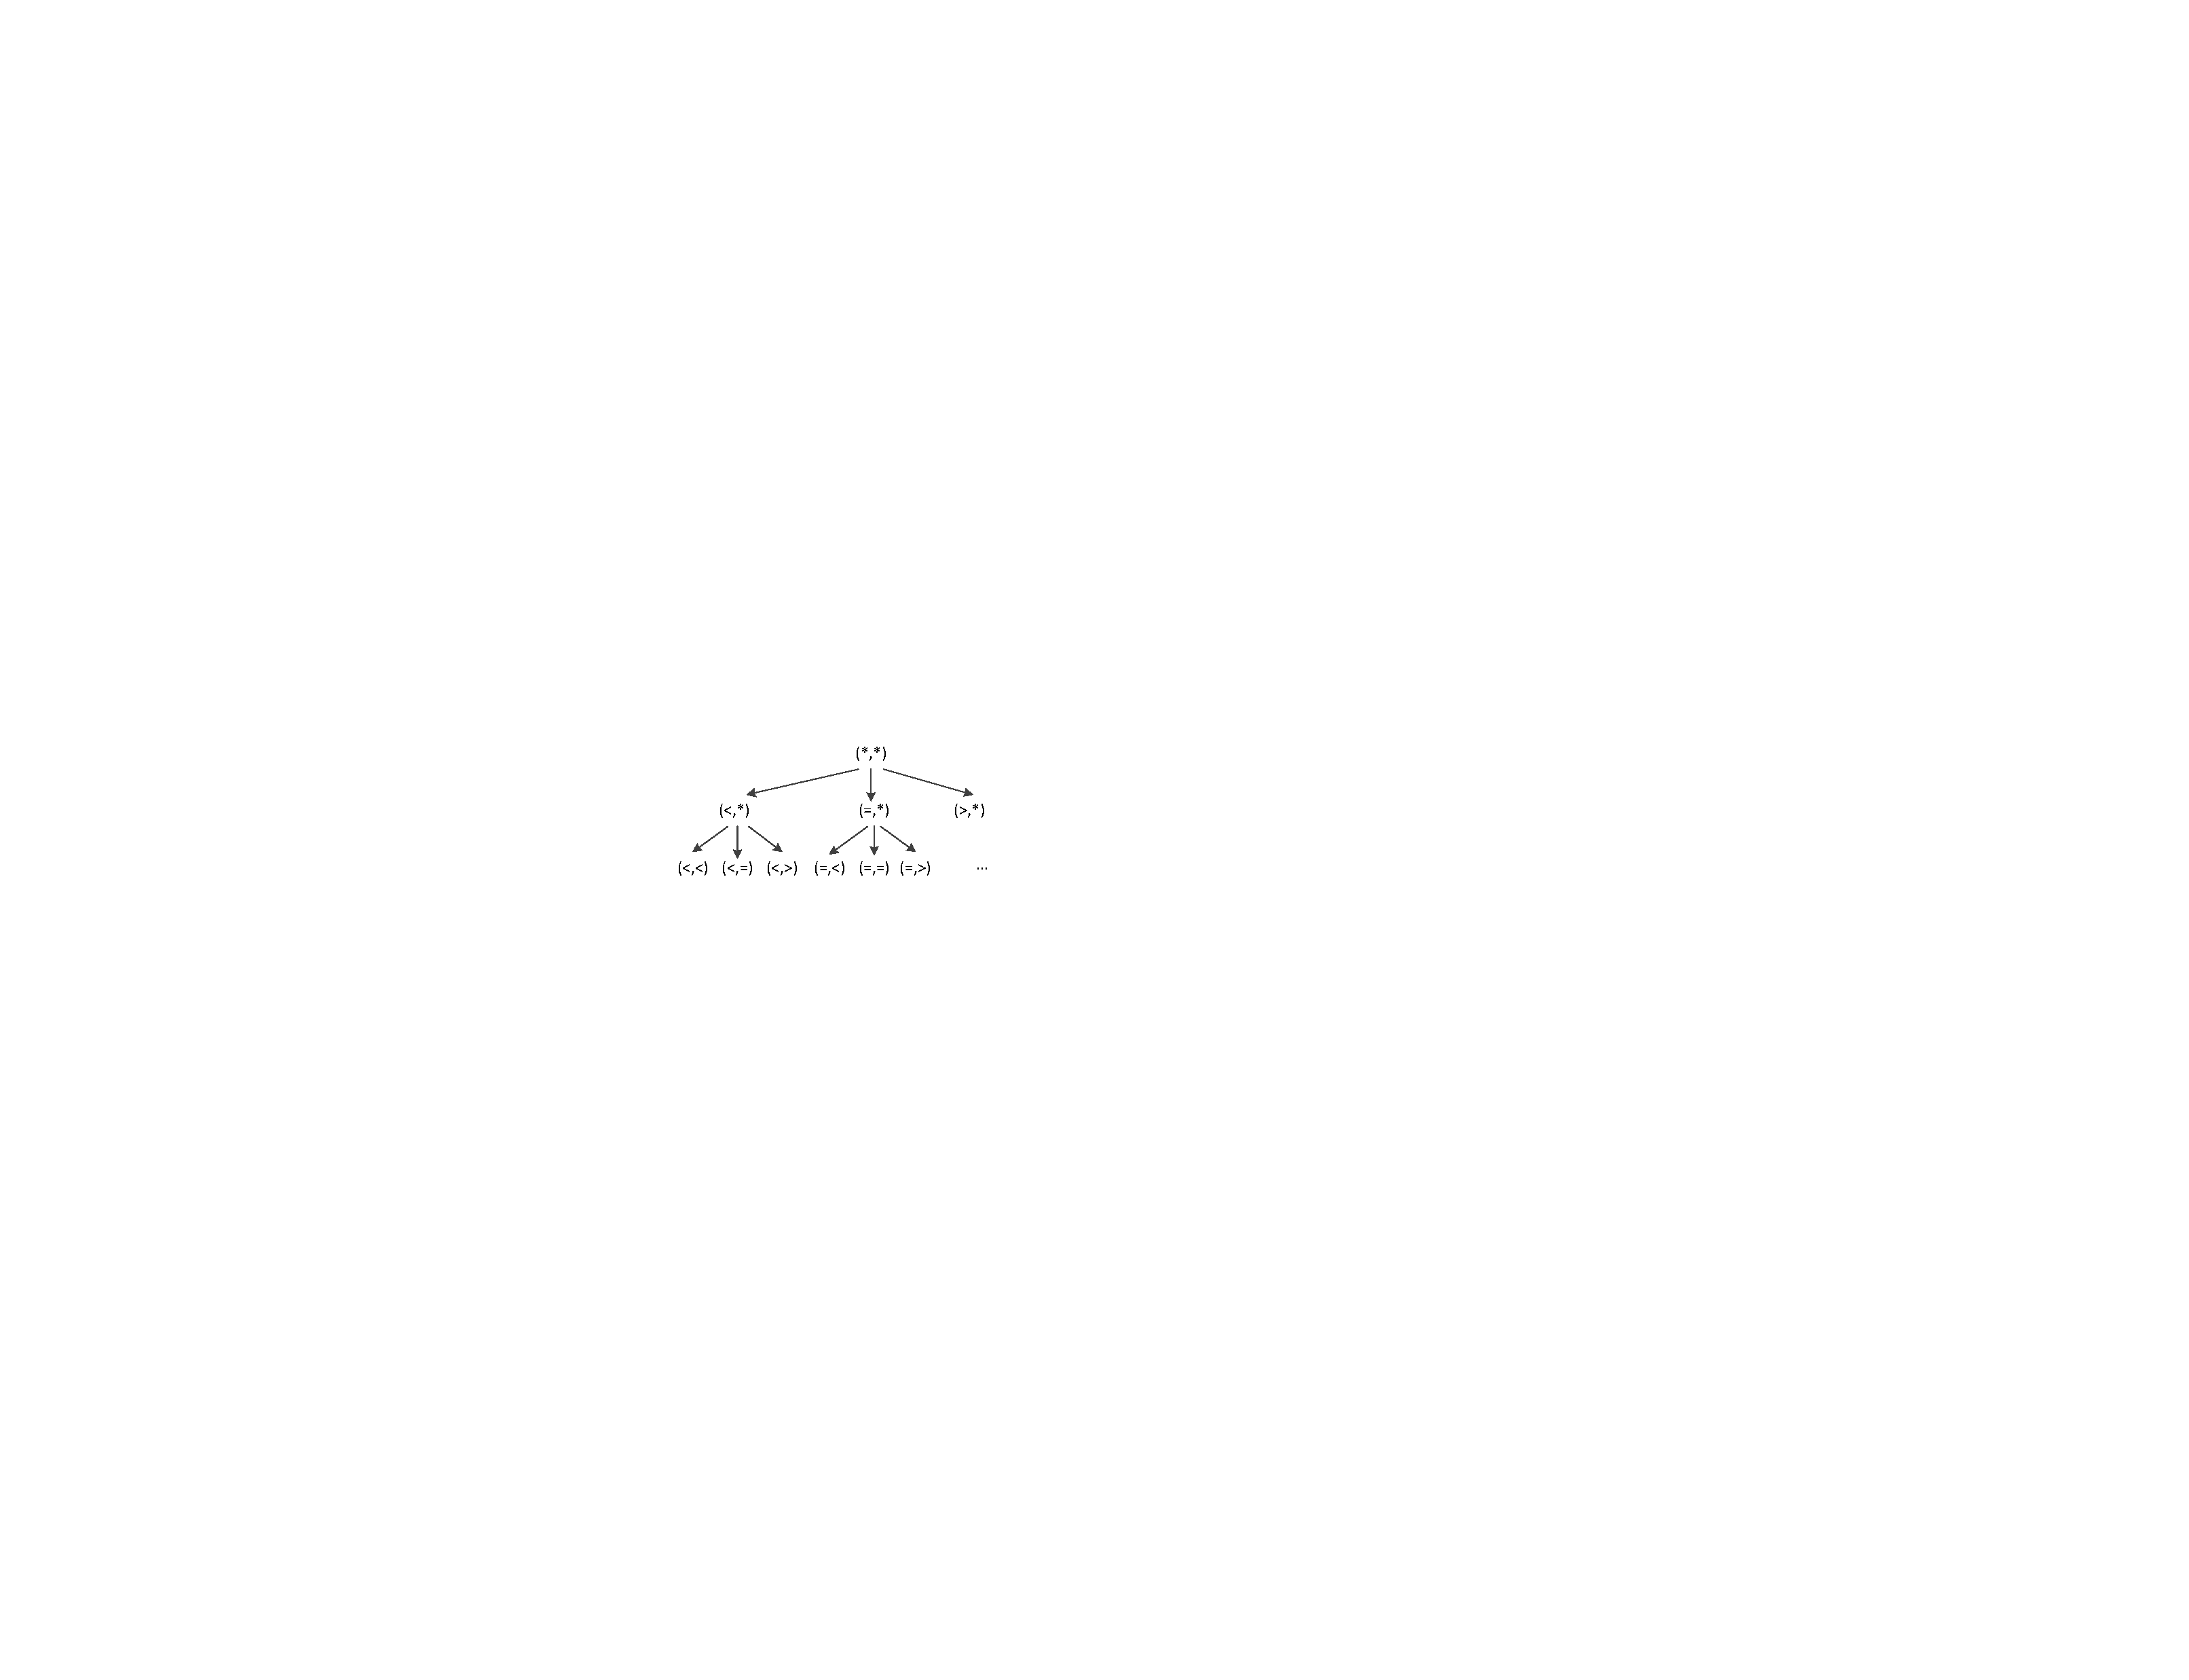
\includegraphics[width=0.6\linewidth]{chap6fig/testingHier.pdf}
\caption{Hierarchy of Dependency Testing for A Two-Level Loop Nest
\label{fig:testingHier}}
\end{center}
\end{figure}
\end{comment}
During the \textit{offline phase}, when the direction vectors based off past execution profiles are assumed to be true, various transformations are performed. If any of these
assumptions is wrong, the generated accelerator will produce wrong results and should not be run. The \textit{online phase} therefore has to verify all the assumptions. More specifically, it needs to check for the presence of any direction vectors which would
invalidate the instruction reordering the \textit{offline phase} has done. 
There are a few main components involved in devising this online checking mechanism:
\begin{enumerate}
    \item Constructing the list of vectors to test.  
    \item Generating C code to test each vector. 
    \item Compiling the vector testing C code into a software routine ($SW_{check}$) %or a small hardware engine ($HW_{check}$)
    \item Running the $SW_{check}$ %or $HW_{check}$ 
    created in the previous step
\end{enumerate}

The first three preparatory steps are all done offline,  along with the synthesis of the accelerators. The last part though, is invoked right before the execution of the
accelerator. Its result determines if the original software binary or the generated
hardware accelerator should perform the computation.

To enumerate the direction vectors to be checked, our flow examines all the transformations performed during the \textit{offline phase}. More specifically, the memory level parallelism and thread level parallelism we have exploited are both going to be explicitly tested. 
%These 
%performed during the \textit{offline phase} 
%include memory-level parallelism, loop interchange and thread-level parallelization. 
Loop pipelining, on the other hand, is
applied conservatively by Vivado HLS and in most cases, aggressive reordering only happens after separation of memory ports. Its validity check is therefore not invoked independently.  

To ensure memory operations can be reordered or even issued through multiple ports, they need to be completely independent from each other as we have explained previously. The vectors tested during the \textit{offline phase}, (*,*...) or (=...,*...) with barrier insertion, are again included for online testing. For thread-level parallelization,
we have to ensure the level at which the iteration space is split does not carry dependency. That is, for any load-store or store-store pair, the direction vector
cannot have leading $``<"$ at this level -- the vector (=...,$<$,*...) must be tested negative. Figure~\ref{fig:testingOnline} illustrates these scenarios with a few simple examples.


\begin{figure}[htp]
\begin{center}

\includegraphics[width=1.0\linewidth]{chap6fig/onlineTesting2.pdf}
\caption{Vectors Used for Online Verification of Parallelism
\label{fig:testingOnline}}
\end{center}
\end{figure}
The actual implementation of these tests was outlined in~\cite{Kennedy:2001:OCM:502981}, which is transcribed into C functions in our flow. One optimization, which
can potentially be applied in both $online$ and $offline$ phases, is to replace Banerjee's test with a simple address range test. When two data structures occupied different ranges in the address space, it is
computationally very cheap to just compare the upper and lower bounds of the accessed addresses. 
However, since Banerjee's test is relatively cheap to evaluate for large sized problems, as will be shown in section~\ref{biev}, this optimization may not be necessary.
%The saving can be significant, as will be shown in section~\ref{biev}.

\begin{comment}

we assume the RTL generation backend, the interconnect and memory subsystem may all be
%aggressively reordering these requests -- by inferring burst accesses or buffering. Therefore, for every pair of accesses whose ordering matters (excluding load-load pair), we check the direction vector (*,*,...), and only continue to execute the accelerator when the test result turns out to be negative. There are also cases where this requirement can be relaxed. In section~\ref{subsec:pmd}, we described how memory barriers are inserted to prevent overly conservative dependency annotation.
%Similarly, in our binary based flow, the online check can be less conservative
%when the ordering of memory operations, each associated with different ports, is partially enforced by barriers.
%An example of this is shown in figure~\ref{fig:withOrWithoutBarrier}. 

In separating 



Memory barriers naturally preclude thread-level parallelization at its level in the loop nest, but memory ports can now be separated as long as the dependency is   carried at or outside the level of insertion. To determine where these barriers
are to be inserted, we uses
 




In a lot of regular computation kernels, data from a multi-dimensional array is read, processed and then written into a different array. Using Banerjee's test, we can obtain negative result for the direction vector (*,*,...), but an easier

Table~\ref{tab:transftest} lists
example tests we need to perform for a three level loop when various transformations were applied.

\begin{table}[htbp]
\caption{Direction Vector Checking for Transformations}
\centering
\begin{tabular}{| c | c | c |  }
  \hline            
 \cline{1-3} 
 Example     & Sequence of Direction  & Description of \\
 Transformations     & Vectors to Disprove & Conditions to Satisfy \\
  %
  %                 & LUT &FFs&  BRAM &  LUT &   FFs      & BRAM   \\
  \hline    
  Separate Memory Ports & (*,*,*)& No dependency\\
  w/o Barriers & &  at every level\\
  \hline
  Separate Memory Ports & (*,*,*) $\rightarrow$ ($>$,*,*) & No dependency below \\  
   with Barriers at level 2 & & the level with barrier\\
  \hline
  Parallelization at & (*,*,*) $\rightarrow$ ($<$,*,*) &\\
  the outermost level & &\\
  \hline     
  Loop Interchange & &\\
 
\hline                                                                                                           

\end{tabular}
\label{tab:transftest}

\end{table}
\end{comment}
\begin{comment}

\begin{figure}[htp]
\begin{center}

\includegraphics[width=0.7\linewidth]{chap6fig/modelEquation.pdf}
\caption{Decision Model Comparing the Performance of Original Binary and the Hardware Implementation for a Two Level Loop Nest
\label{fig:modelEquation}}
\end{center}
\end{figure}
\end{comment}


%FIXME --- this doesn't quite work
%These tests certainly introduce runtime overhead into our system. 
%Depending on how much computation is going on in the target loop nest, these tests may be incurring a significant runtime overhead. 

In general, how significant a run time overhead the Banerjee's tests incur depends on how much computation is going on in the targeted loop nest.
%On the other hand, they are highly parallelizable and can be potentially offloaded to the hardware completely. 
They certainly reduce the overall speed up attainable with the accelerator and for smaller loop nests, they may completely nullify the benefit of computation offloading. %Together with the cost of data transfer, which will be described in section~\ref{dtransfer}, these overheads can nullify the benefit of computation offloading.
It is thus useful to estimate the performance of the hardware accelerator and the software binary when executing loop nests of different sizes. More specifically, to decide if the amount of computation justifies the invocation of the  $SW_{check}$ and the accelerator, we need to find the size of iteration space $I$ such that

\begin{equation}
\label{checkWorth}
  S_t(I)-H_t(I) >>  D_t
\end{equation}


%Fortunately, we can devise a simple model to
%evaluate if the amount of computation justifies the invocation of the validity check and accelerator:
$S_t(I)$ and $H_t(I)$ are %a pair of simple 
functions predicting the execution time of the loop nest in software binary and hardware accelerator respectively, while $D_t$ denotes the 
runtime overhead of performing parallelization validity check($SW_{check}$). % or $HW_{check}$. 
Note that $D_t$ does not vary with the size of $I$, but the dimensionality of it, which is known during compile time.
On the other hand, to accurately predict how the binaries or accelerators' performance vary with $I$ can potentially involve complex mechanisms.
Various processor architecture features, interaction with the memory subsystem, or the the paradigm the accelerator synthesis flow follows can all make a big difference for a particular workload. Simulation based approaches~\cite{Oyamada:2007:SPE:1323351.1323449}\cite{Meswani:2013:MPP:2493921.2493922}, which may be suitable for design time exploration, are certainly too costly for automatic run time decision making. 
One alternative is to measure the actual execution for the software implementation and hardware accelerators (with the online checks) over different sized input, and record the smallest $I$ where computation offloading actually provides benefit. As larger iteration space further amortizes the performance degradation caused by the online checks, invocation of accelerators should lead to speed up as well.
We can then reduce the decision model to a series of simple arithmetic and comparison operations involving the loop bounds and the recorded $I$, which can be evaluated during the $online$ phase with negligible impact on the overall execution time.

%and interpolate to obtain the cross over points where the computation offloading starts to provide benefits. The model is then
%reduced to a series of simple arithmetic and comparison operations involving the loop bounds, which can be evaluated during the $online$ phase with negligible impact on the overall execution time. An example of this is shown in figure~\ref{fig:modelEquationMM}.  

\begin{comment}
To accurately estimate these quantities by statically examining the instructions and HLS generated schedules is rather challenging.

In this work, we sacrifice the prediction accuracy and construct $S_t$ and $H_t$ to be just simple polynomials of elements in $I$, involving only basic arithmetic operations on the loop bounds. Consequently the impact on the execution time when they are evaluated during the $online$ phase is minimal.  An example is shown in figure~\ref{fig:modelEquation}, where the coefficients are statically computed from instruction counts in the software binary and operation schedules of the HLS generated accelerator, with a factor to account for off chip memory accesses. The 
\end{comment}

%given the size of the iteration space. Meanwhile $T_t$ and $D_t$ are functions estimating the time used for data transfer and the parallelism validity check. 

%This model is again generated during the offline phase and executed during the online phase.
%An example model is shown in figure~\ref{fig:modelEquation}. 
%Evaluating this model takes time as well, but since it involves only a few basic arithmetic operations on
%can be reduced to a set of quick checks on 
%the loop bounds, its impact on execution time would be rather small. Note the coefficients used
%in these models, at the moment, are generated by profiling the actual execution of software binaries and FPGA accelerators. 
%To accurately estimate these quantities by statically examining the instructions can be rather challenging for both the software implementation and the hardware
%accelerator. Various processor architecture features, interaction with the memory subsystem, or the the paradigm the accelerator synthesis flow follows can all make a big difference for a particular workload. We have thus chosen to empirically gather data and annotate these models rather than design a accounting framework generating numbers from a static fragment of instructions. 



\begin{figure}[htp]
\begin{center}
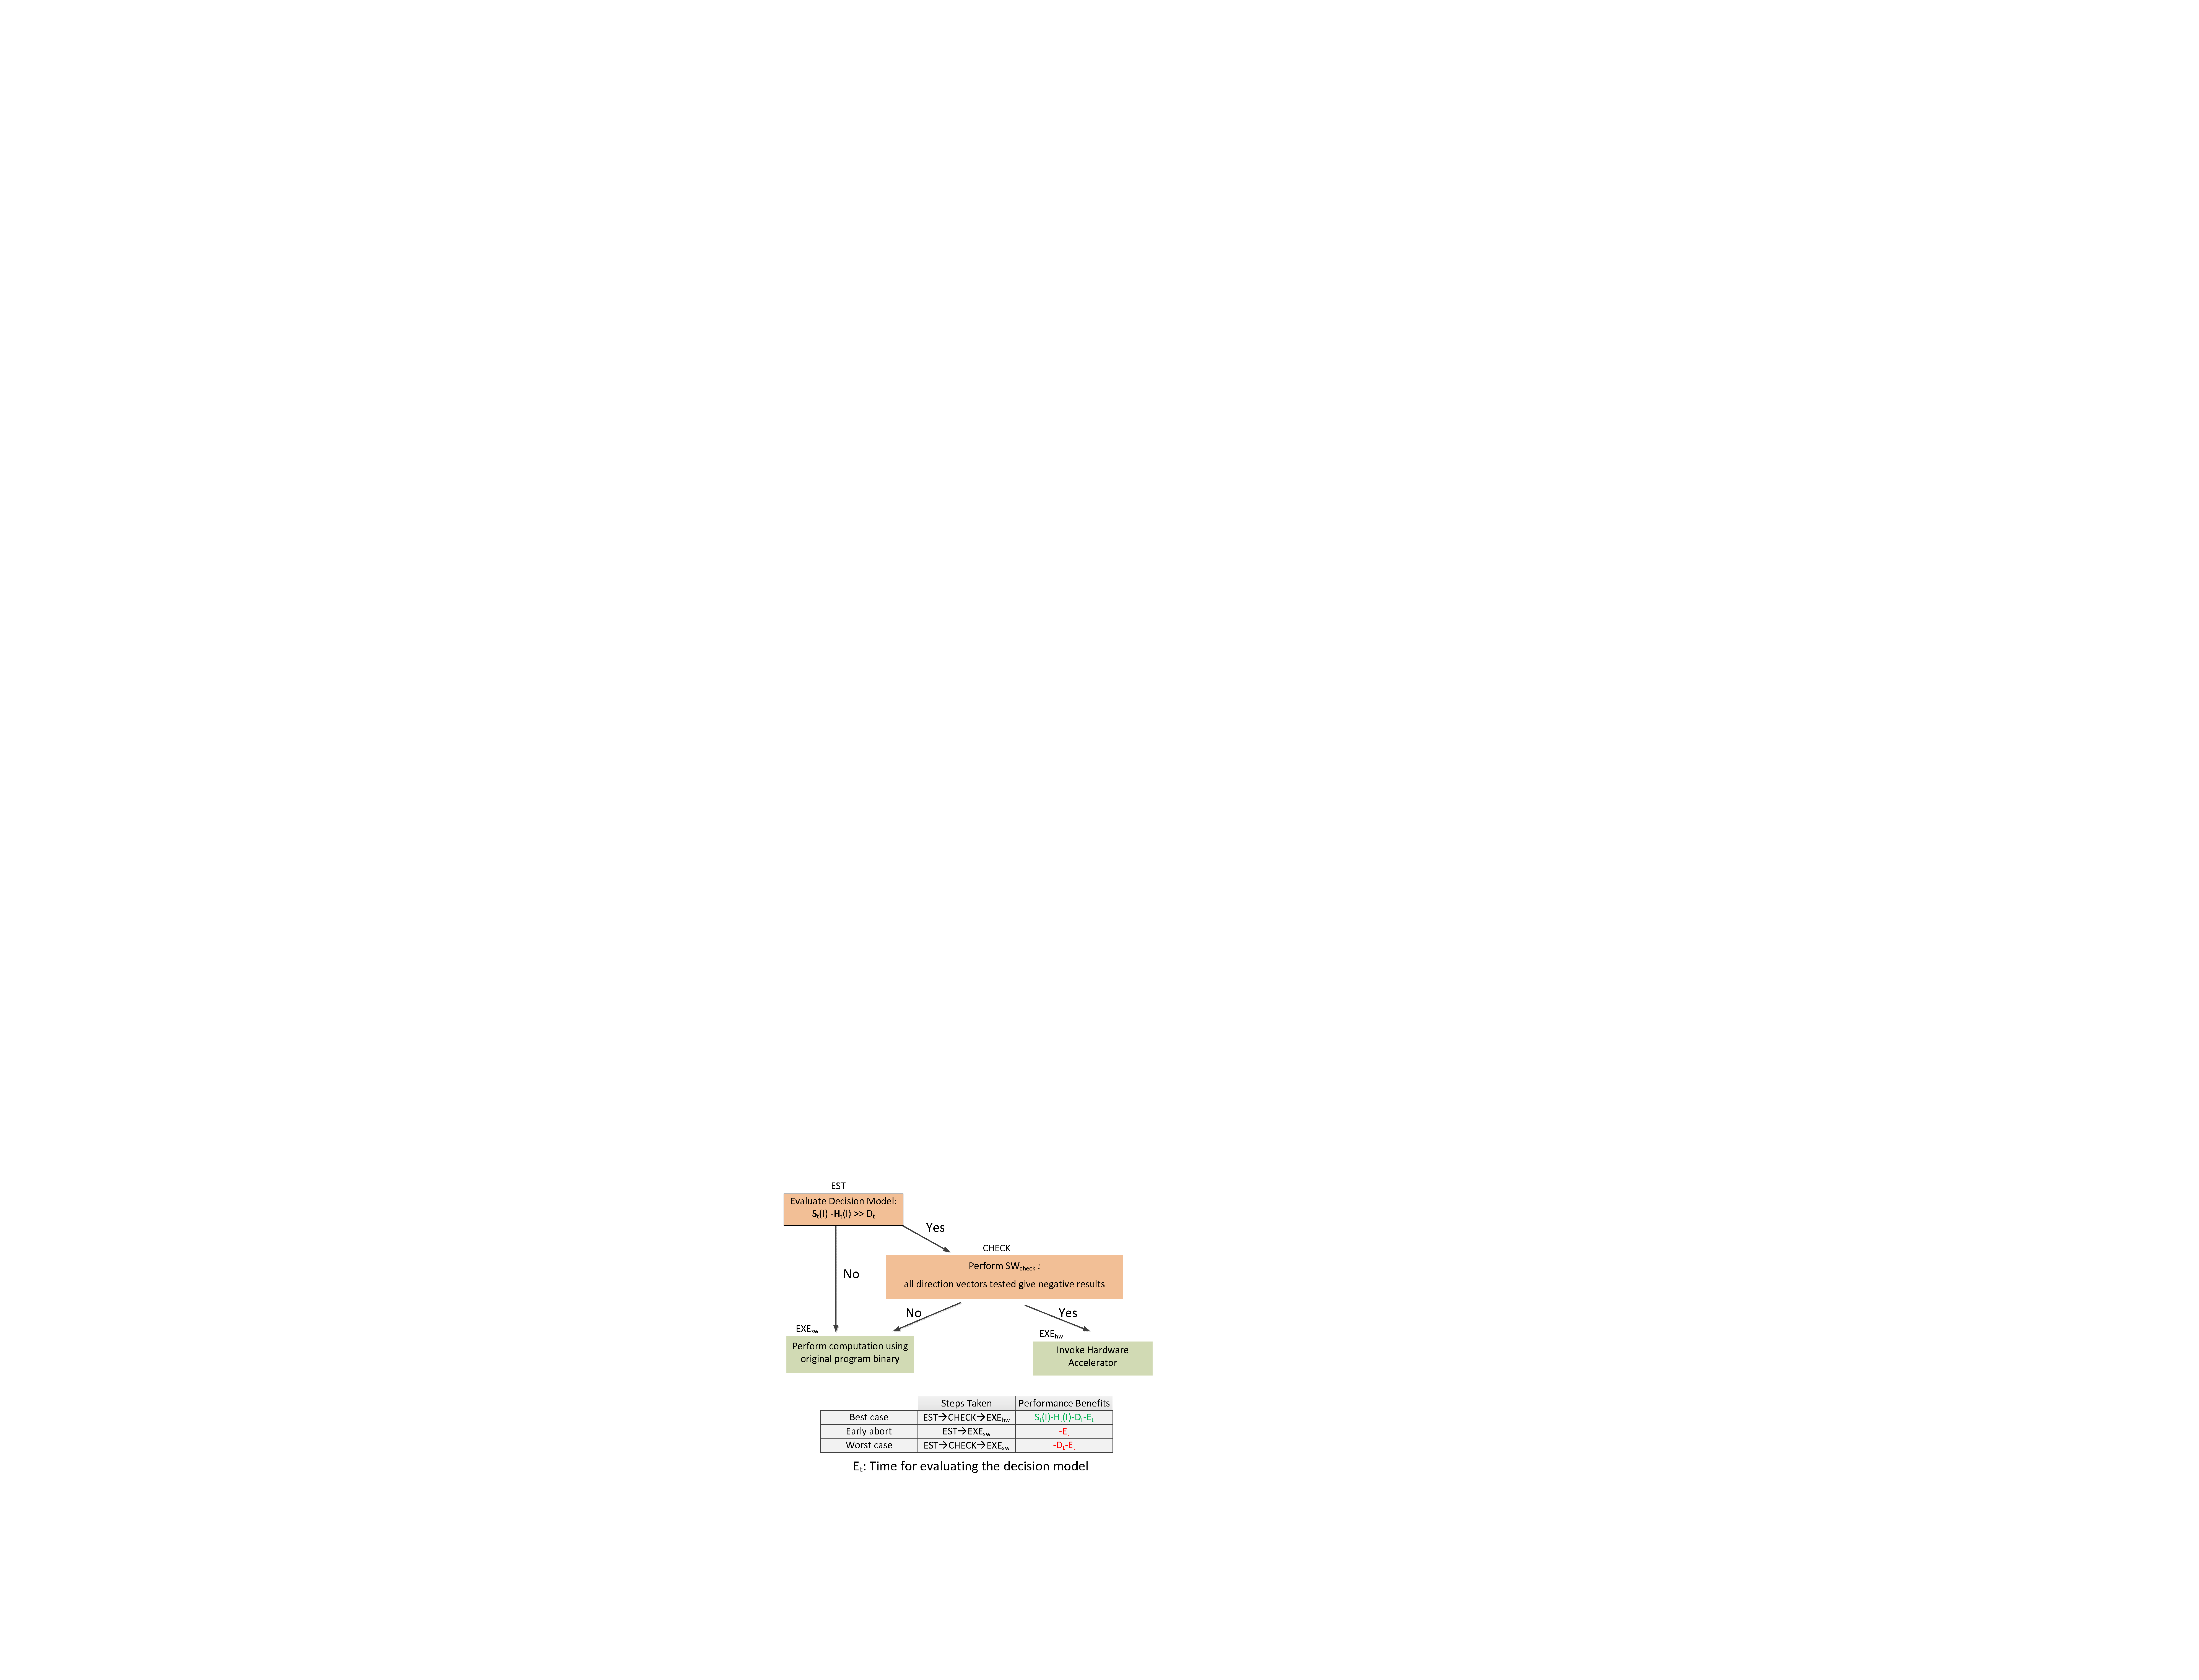
\includegraphics[width=0.9\linewidth]{chap6fig/mainStepsExecution.pdf}
\caption{Main Steps in Running Accelerator-augmented Program Binaries
\label{pieces-doModel-doOnline-doInvoke}}
\end{center}
\end{figure}


To summarize, the main steps for the execution of the accelerator-augmented program binaries is illustrated in figure~\ref{pieces-doModel-doOnline-doInvoke}. %As the decision model is always evaluated, its cost is incurred even if the validity check is not performed. It is therefore advisable to only apply our approach to loop nests whose past behavior exposes sufficiently sized iteration space. 
The worst case scenario is  when all the parallelism checks are performed and dependency vectors invalidating the parallelization are found. This should rarely occur, as previous studies found dependence behavior almost never changes with the data input~\cite{Tournavitis:2009:THA:1542476.1542496}\cite{Bhattacharyya:2013:IMU:2523721.2523775}.

%In the worst case, both the decision model and the validity check are run but the 
%in the worst case, when
%the accelerated version of the loop nest is never executed, there would be a slight increase in execution time. It is therefore advisable to only apply our approach to loop nests whose past behavior exposes sufficiently sized iteration space.


%The performance estimates shown in figure~\ref{fig:fpgaparal} do not take into account the data access latency
%if they have to be brought in from off-chip RAM. By performing transformations
%to maximize data reuse, it can increase the ratio of computation v.s. off-chip memory bandwidth usage. 


\begin{comment}

The range of addresses we would like to copy
to the FPGA device needs to be explicitly specified, the size of the


We need to explicitly specify the range of address we would like to copy to the
FPGA device from the CPU
In this case, we rely on the regularity of the memory access patterns in our targeted loop nests to derive a concise representation of the accessed address stream. 




allows us to easily decouple the management of data transfer from the actual computation.
We can derive concise representations of the accessed addresses by the accelerator without actually running it. 
If the FPGA does not have direct access to the CPU memory, then explicit
data transfer is required. This is usually higher cost






Locality driven optimizations performed
described in section~\ref{}




The analyzability required for coarse grained parallelism discovery 
already provided us with 

also
facilitates the calculation of the exact memory footprint for the accelerated computation. 


More specifically, the addresses stream can be 




In addition, many processor centric systems 
use virtual memory to facilitate programming and manage the memory hierarchy, 






The approach described in chapter~\ref{decoupleChap} may be used but provides little advantage for these computation. 






 

%with 
%a particular parallel architecture as the target may be unnecessary. For %instance, vectorizing compilers may perform loop interchange to have 

%An interesting aspect of 

Our parallelization engine attempt to  

\end{comment}

\begin{comment}
The variety of hardware templates gives another dimension in the accelerator design space, in addition to the software domain optimizations like loop interchange, loop tiling etc. 

For a specific loop nest, whose dependence graph is constructed using the information acquired through dependency analysis, there are multiple
possibilities 

As mentioned in section~\ref{sec:fdtp}, we use Banerjee's tests to find 
direction vectors between different statements in the loop nest. There are 
a few additional techniques employed to make runtime check cheaper





One particular important aspect, in ensuring the efficient execution of the accelerators, is in the management of data transfers. 
The regularity of the memory access patterns in our targeted loop nests
allow us  to easily decouple the transfer of data from the computation. 
The analyzability required for coarse grained parallelism discovery also
facilitates the calculation of the exact memory footprint for the accelerated computation. More specifically, the addresses stream can be 


The approach described in chapter~\ref{decoupleChap} may be used but provides little advantage for these computation. 
\end{comment}

\begin{comment}
At a high level, the approach we are proposing in accelerating program binaries
can be divided into two phases. For an acceleratable loop nest, we first examine
it's past execution profile to extract necessary information to perform dependency analysis offline. After obtaining the dependency direction vectors between statements, we can then perform parallelization and the actual accelerator synthesis. 
Now, whether the generated accelerator is consistent
with the semantics of the original program depends on if the dependency
testing results remain true when the actual execution happens. This is our
second phase, where an online check is performed to confirm the validity
of the assumed parallelism.
\end{comment}









\section{Accelerator Integration with the Application Binary}
An important part of integrating the accelerator with the application binary is the transfer of machine states between the FPGA and the CPU. As the memory are shared between them, updates to non-stack variables do not need to be explicitly handled. On the other hand, as the registers and stack variables are converted into local variables in the C code used for accelerator generation, their changes are not automatically propagated to the processor side. To resolve this issue, a special data structure is used to store the final values of these variables. A small segment of code, consisted of a series of memory writes, is also inserted into the C function before it gets processed for accelerator synthesis, this is illustrated
in figure~\ref{}.

On the processor side, to replace the loop nest in the original program binary with the generated decision model evaluation, validity check and accelerator invocation subroutine, Dyninst is again used. The abstract representation of the application binary is rather similar whether the program is running as a process or statically
stored in the disk. Consequently, the main parts of the ``mutator"  can work both dynamically, with a already-running process getting patched to have improved speed, or statically, with application binary being rewritten to run faster next time it gets executed. 

As mentioned earlier, instrumentation code in Dyninst is organized into ``snippet". It is certainly possible to create the online checks, accelerator initialization and invocation using these snippets, but a more convenient method is to generate
a separate set of functions encapsulated in a shared library,
which also contains a top level wrapper function chaining all the steps performed during the $online$ phase. Dyninst allows for addition of library dependencies to existing binaries, which can then use the newly created functions through inserted simple snippet performing function calls.



Other than the steps shown in figure~\ref{pieces-doModel-doOnline-doInvoke}, the wrapper function is also responsible to extracting the run time constant for the accelerated loop nest.
The register values are read out using inline assembly code,  while the stack variables are dereferenced through offsetted stack pointer (with the inserted call instruction properly accounted for). The values corresponding to loop bounds are fed to the decision model while the coefficients are supplied as
parameter for the $SW_{check}$ routine. Then, the accelerator initialization and invocation are performed using these values as arguments. 
Finally, after the accelerator execution, the registers and stack variables updated by the original binary would contain stale values. The wrapper function is  responsible for repopulating these registers/memory locations with new values extracted from the special data structure written to by the accelerator.

An example of a wrapper function is shown in figure~\ref{}.

The original binary is also modified using the PatchAPI in Dyninst. The first instruction of the loop nest is replaced with a call instruction invoking the wrapper function from the
%In the original binary, we replace the first instruction of the loop nest with a function call invoking the wrapper function
 shared library. An unconditional jump is inserted immediately after the call, targeting the successor basic block of the loop nest. 
 
 It should be noted that our flow is a best effort attempt to ensure the machine states in the CPU remain the same whether the original software binary or the FPGA accelerator gets activated. There are CPU specific mechanisms like precise exception for which our flow has no support for. 

%Using the PatchAPI in Dyninst, we can replace the first instruction of the loop nest with a function call invoking the generated subroutine from the shared library. Immediately after this function call, an unconditional jump is inserted, targeting the successor basic block of the loop nest. 


%Dyninst is capable of performing both dynamic instrumentation and static rewriting of program binaries. In our flow, we use it as a static binary rewriter so the parsing and instrumentation overhead is amortized. 


% insert figure for dyninst, 
%FIXME




%\subsection{The Binary Rewriting Flow}
%In Dyninst's terminology, the binary to be modified is called the ``mutatee" while the program performing the rewrite is the ``mutator". Our flow implements a mutator to redirect the mutatee's execution to the FPGA accelerator. 
%The main mechanism we rely on is the function replacement capability in Dyninst.
%It can redirect all invocation of a function in the mutatee to a new implementation by inserting a non-return jump in the beginning of the old function body. Alternatively, it can rewrite the destination of specific call sites so the execution can be steered according to the context. 
%In our flow, during the collection of runtime profile, a map was built to associate the amount of computation a particular loop nest performs with the invocation locations of its container function. Only for call sites which triggers large amount of computation, as certified by equation~\ref{checkWorth}, the function invocations are redirected to the new implementation, while the rest still invokes the original binary. 


%As the source code of $func_{accel}$ is generated separately during $offline$ phase
%new function implementation is generated separately, we
%and compile into a shared library, our flow adds library dependency to the static binary using DyninstAPI to ensure the new implementation would be made available by the dynamic linker.

%Before and after the loop nests, which got turned into the validity check/invocation of accelerator contained in $fun_{core}$, $fun_{orig}$ often contains small amount of computation and data accesses which are essentially copied into $func_{accel}$ 



%Starting the accelerator involves transferring a small set of machine state from the processor size to the programmable logic. Register values and stack variables
%often needs to be turned into the arguments of the function going through HLS so they can be written by the accelerator invocation stub. FIXME: try this -- move
%registers/stack variable into variables and pass to a function......

%A more detailed structure of a typical $func_{accel}$ is illustrated in ~\ref{fig:detailWholeFunc}, which also shows how it gets used when an edited binary is executed.
\begin{figure}[htp]
\begin{center}
\includegraphics[width=0.7\linewidth]{chap6fig/detailWholeFunc.pdf}
\caption{Parts of the Replacement Function
\label{fig:detailWholeFunc}}
\end{center}
\end{figure}





\section{Experimental Evaluation }
\label{biev}

To validate the feasibility of our approach, binaries
of a few compute intensive programs were pushed through our flow.
We perform our experiments on the same hardware setup (Zynq-7000 XC7Z020 FPGA SoC on Zedboard) as the one used in 
chapter~\ref{decoupleChap}. Using the Xilinx tool chain for RTL generation and FPGA mapping, we configure the timing constraints   
and the final clock frequency %used in the final designs are also configured
in the same way as the previous experiments. Vivado HLS is set to target 8ns clock period while the highest clock frequency achieved after place and route is used for performance benchmarking. The baseline of our performance comparison is the software binary running on the ARM core in Zynq. %The conventional accelerator and 
A decoupled computational pipeline is first generated, directly from the C function produced by our preprocessing step, and connected to the HP port before further design space exploration is attempted.


As the targeted regions of the application binaries are regular loop nests, our flow can be configured to take advantage of coarse grained parallelism. In our experiments, we  gradually increase the amount of
thread level parallelization by more aggressively splitting the iteration space, as described in section~\ref{subsec:cgp}. Meanwhile, as the Zynq SoC contains multiple HP ports connecting the programmable logic to the memory, the amount of bandwidth available to the hardware threads can be varied. Thus for every benchmark, we also increase the number of HP ports enabled to quantify the effects it has on the overall performance of the accelerators.

Another important component of executing accelerators generated from program binaries, as discussed in section~\ref{onlinephase}, is the set of online checks which must be run before the accelerators are invoked.
%Equation~\ref{checkWorth} is evaluated first to estimate if the overhead of parallelization validity check would have out-weighted the benefit of running the FPGA accelerator. The input to this equation is the size of the iteration space, or more specifically, the upper and lower bounds for each level of the loop nest. 
The size of the iteration space, or more specifically, the upper and lower bounds for each level of the loop nest, are first examined to estimate if the overhead of parallelization validity check would have out-weighted the benefit of running the FPGA accelerator.
The actual Banerjee's test is then performed. The cost of completing these computation during run time is also evaluated for every benchmark in this section.

Note the purpose here is not to highlight, in absolute terms, how fast we can perform the computation. There are many techniques which can be applied, either manually or through compiler optimizations, to each individual benchmark. We just want to demonstrate how some of those can also be used, without source code modification and recompilation, to take advantage of the FPGA fabric to achieve good speed up.


%The pipeline parallelism in 
%In addition to the pipeline parallelism exploited by our flow, for regular 
%kernels we are targeting in this chapter, coarse grained parallelism can be extracted and exploited. 

%By instantiating multiple pipeline and activate them in parallel, we can increase the overall throughput and complete the accelerated region 


\subsection{Performance Results}

\subsubsection{Benchmark 1: GemsFDTD}
The first application, GemsFDTD, is
a general electromagnetic solver which solves the Maxwell equations in 3D in the time domain using the finite-difference time-domain (FDTD) method. Every timestep,
an update of the E-field and H-field, stored in three dimensional arrays, are performed. Originally coded in Fortran 90, this benchmark would not have been directly synthesizable using the Xilinx tool chain without the binary based flow, even though the workload is particularly suitable for FPGA acceleration. 


%As the main portion ($>95$\%) of the execution time is spent in the timestepping function, where triple-nested loops are used to compute  the E-field from H-field/H-field from E-field, this part of the program binary is identified and accelerated by our flow. 
Two triple nested loops are  are used to compute  the E-field from H-field/H-field from E-field.
Their memory footprint is determined by the size of the grid used to represent the space. The data structures representing the fields in 3D scales up cubically with the number of units in each dimension. For our performance comparison, grids of multiple different sizes are used. 
%a grid with 100 units on each dimension is used. 
Figure~\ref{fig:fdtdPerf} shows the performance of the decoupled computational pipeline for different problem sizes. Coarse grained parallelism at the outermost loop is also exploited to split the iteration space into two halves. 
All numbers are normalized to the processor performance, reflecting improvement over the software binary.
%of different design points we have implemented for the accelerator.

\begin{figure}[htp]
\begin{center}
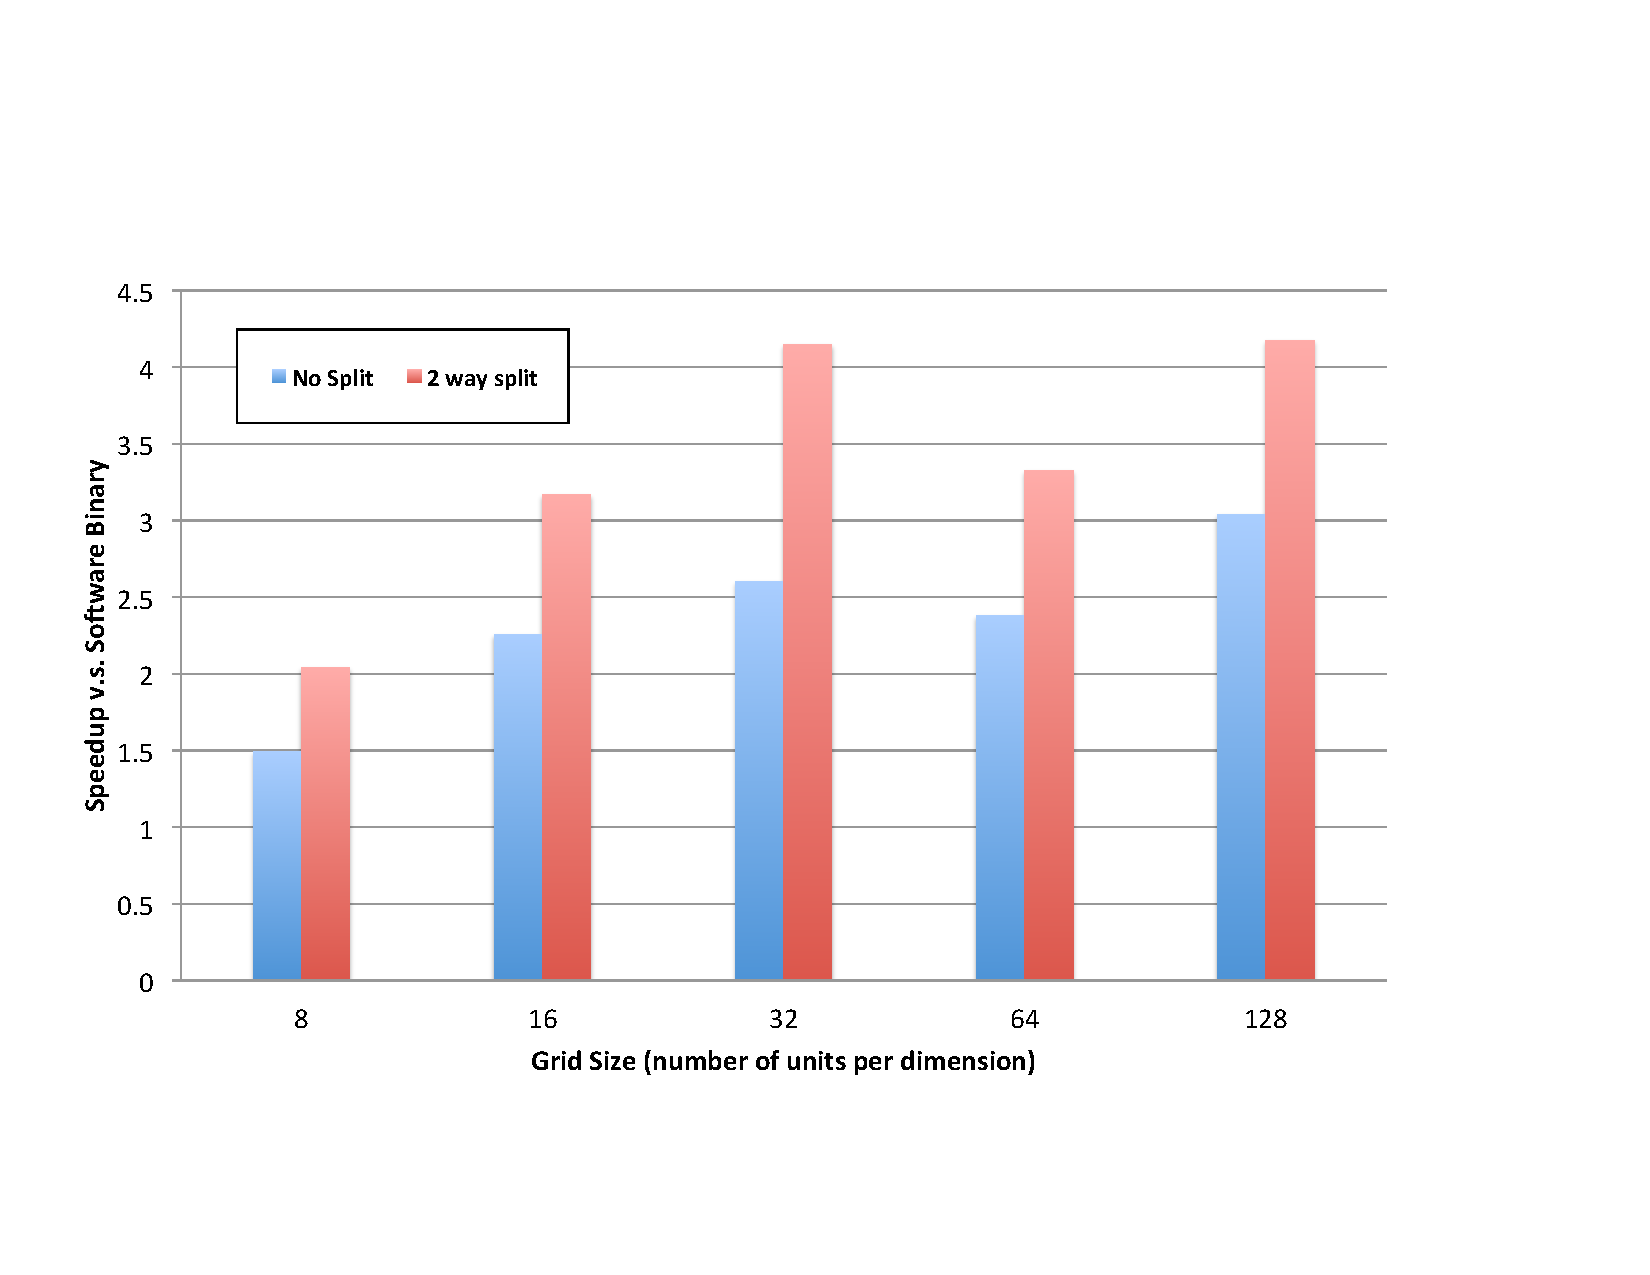
\includegraphics[width=1.0\linewidth]{chap6fig/fdtdPerformance.pdf}
\caption{Performance Comparison of Decoupled Computational Pipeline and Software Binary for GemsFDTD
\label{fig:fdtdPerf}}
\end{center}
\end{figure}

The pipeline implemented in programmable logic, despite running at a fraction of
the processor's clock frequency, is able to outperform the software binary. Its performance advantage is also more pronounced for larger sized grid as the constant cost of initializing the accelerator gets amortized over a greater amount of computation. For a space of 128x128x128 units, the computational pipeline achieves a 3x improvement over the processor, while only 1.5x speedup is observed when targeting an 8x8x8 space. In addition, when we take advantage of the coarse grained parallelism, the performance goes up even further. With the iteration space split two ways, the generated pipeline achieves 4.2x speedup. More aggressive splitting of the loop nest results in resource utilization greater than 100\% for our platform and is therefore not mapped on actual hardware.

%With one port to the memory  enabled, the speed up reaches 6.7X when the loop nest is parallelized to two threads. Enabling a new HP port and dedicating it to the second thread further increases the speed up to 9.5X. More coarse grained parallelism results in resource utilization greater than 100\% for our platform and is therefore not mapped onto actual hardware. 

\begin{figure}[htp]
\begin{center}
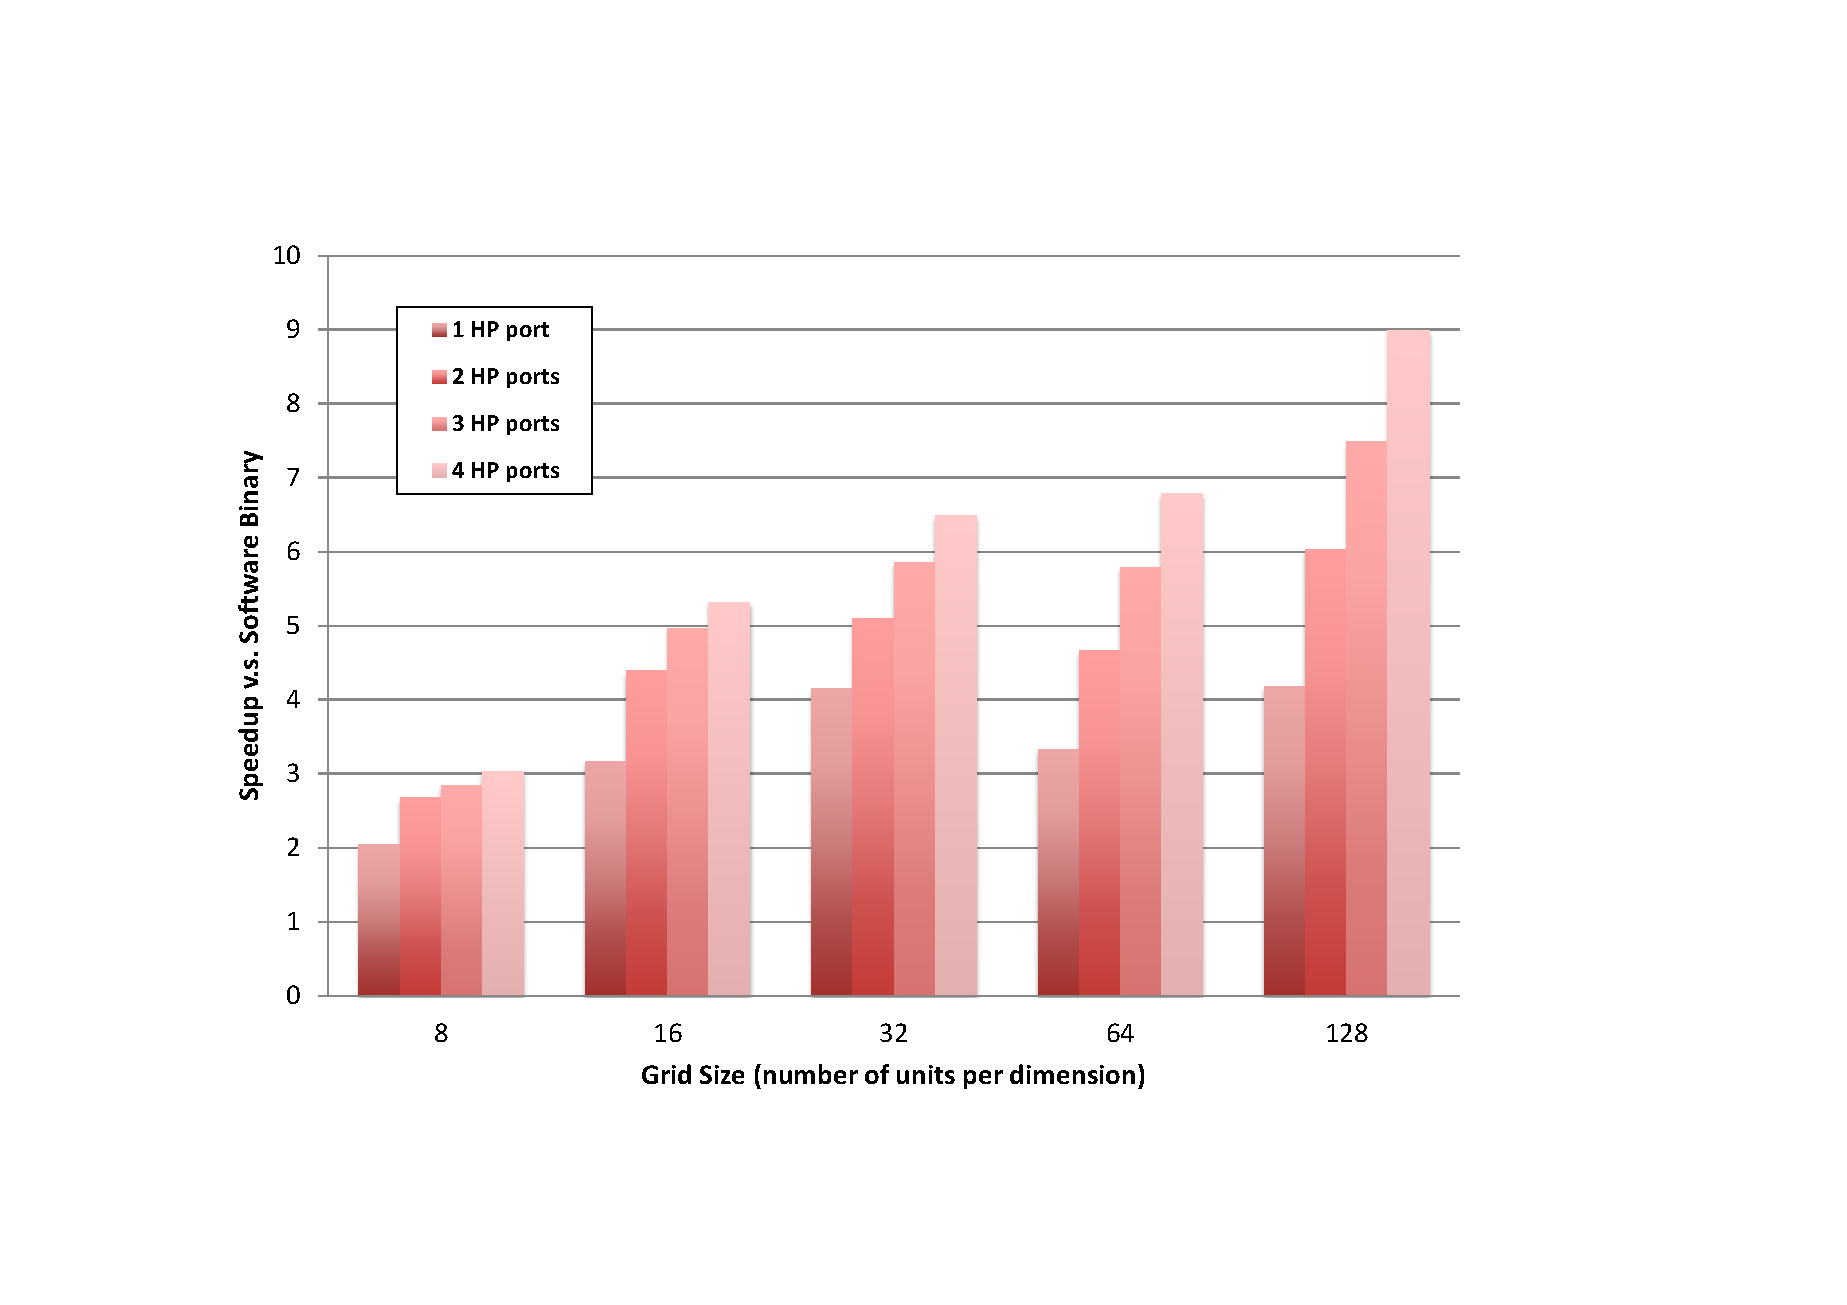
\includegraphics[width=1.0\linewidth]{chap6fig/fdtdHP.pdf}
\caption{GemsFDTD Performance with 2-Way Split of the Iteration Space and Different Number of HP Ports
\label{fig:fdtdHp}}
\end{center}
\end{figure}

The HP ports and associated interconnect IPs providing data access to the computational pipeline are often the limiting factor for the performance. Figure~\ref{fig:fdtdHp} shows how the speedup changes as we vary the number of ports to memory. Evidently, the compute capacity provided by the pipeline with a 2 way split of the iteration space can consume data faster than the rate sustained by a single HP port. As we enable more ports, across which the data access interfaces of the pipeline are evenly distributed, the performance increases further. For the largest problem size, with all HP ports to the programmable logic enabled, close to 9x speedup is achieved.



\begin{figure}[htp]
\begin{center}
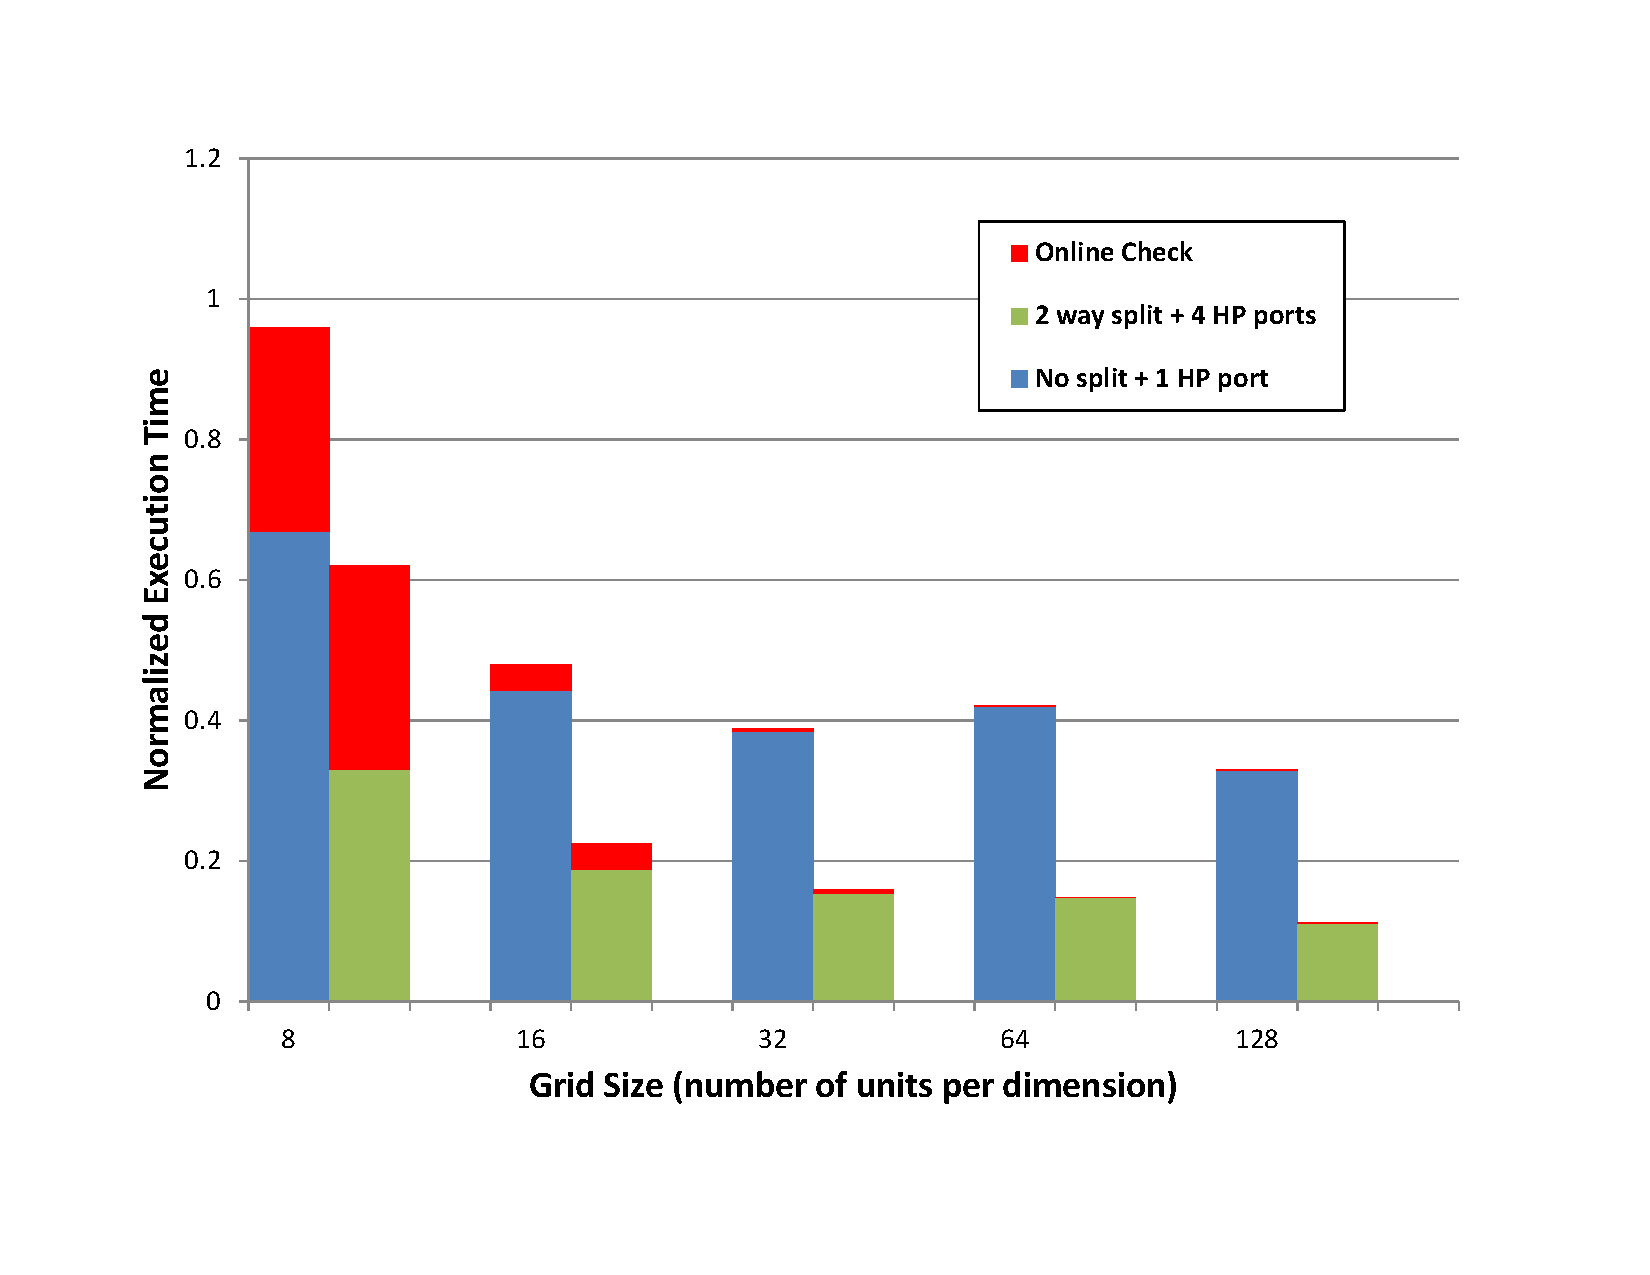
\includegraphics[width=1.0\linewidth]{chap6fig/fdtd2phase_2.pdf}
\caption{Overall Execution Time of Accelerators with Online Checks for GemsFDTD
\label{fig:fdtdOverhead}}
\end{center}
\end{figure}

Shown in figure~\ref{fig:fdtdOverhead} is the overall execution time of the fastest and slowest accelerator configurations, including the overhead of all online checks. The execution time is normalized to that of the software binary and the lower the bar, the faster it is relative to the unaccelerated version. As expected, for small sized problems, the online checks can be expensive, relative to the execution time of both the software and the hardware accelerator. However, as the problem size gets larger and the loop nest itself takes up more time, the overhead becomes negligible. For this benchmark in particular, even using the slowest accelerator configuration for the smallest grid we have tried, the performance advantage of the accelerators is big enough to outweigh the overhead introduced. 

\subsubsection{Benchmark 2: Matrix Multiplication}
Matrix multiplication is an computation kernel which has been examined and optimized in many different contexts. %The cache performance, which can be quite different on the processor side as we vary the size of the matrices, plays an important role in the overall execution speed. 
In this experiment, we use a vanilla implementation to compare the FPGA accelerator against the processor for different problem sizes. Our data therefore covers various scenarios, from when all operand matrices can fit on the cache and the processor has cache hit most of the time, to the case where no data in a cache line is accessed more than once. 
Meanwhile, the accelerators being compared do not have any caches instantiated using the programmable logic. As we are only mirroring the memory access patterns of the processor instead of applying additional high level transformations such as blocking, the instantiation of expensive caches on the FPGA provides little overall performance gain for large sized problems. 

\begin{figure}[htp]
\begin{center}
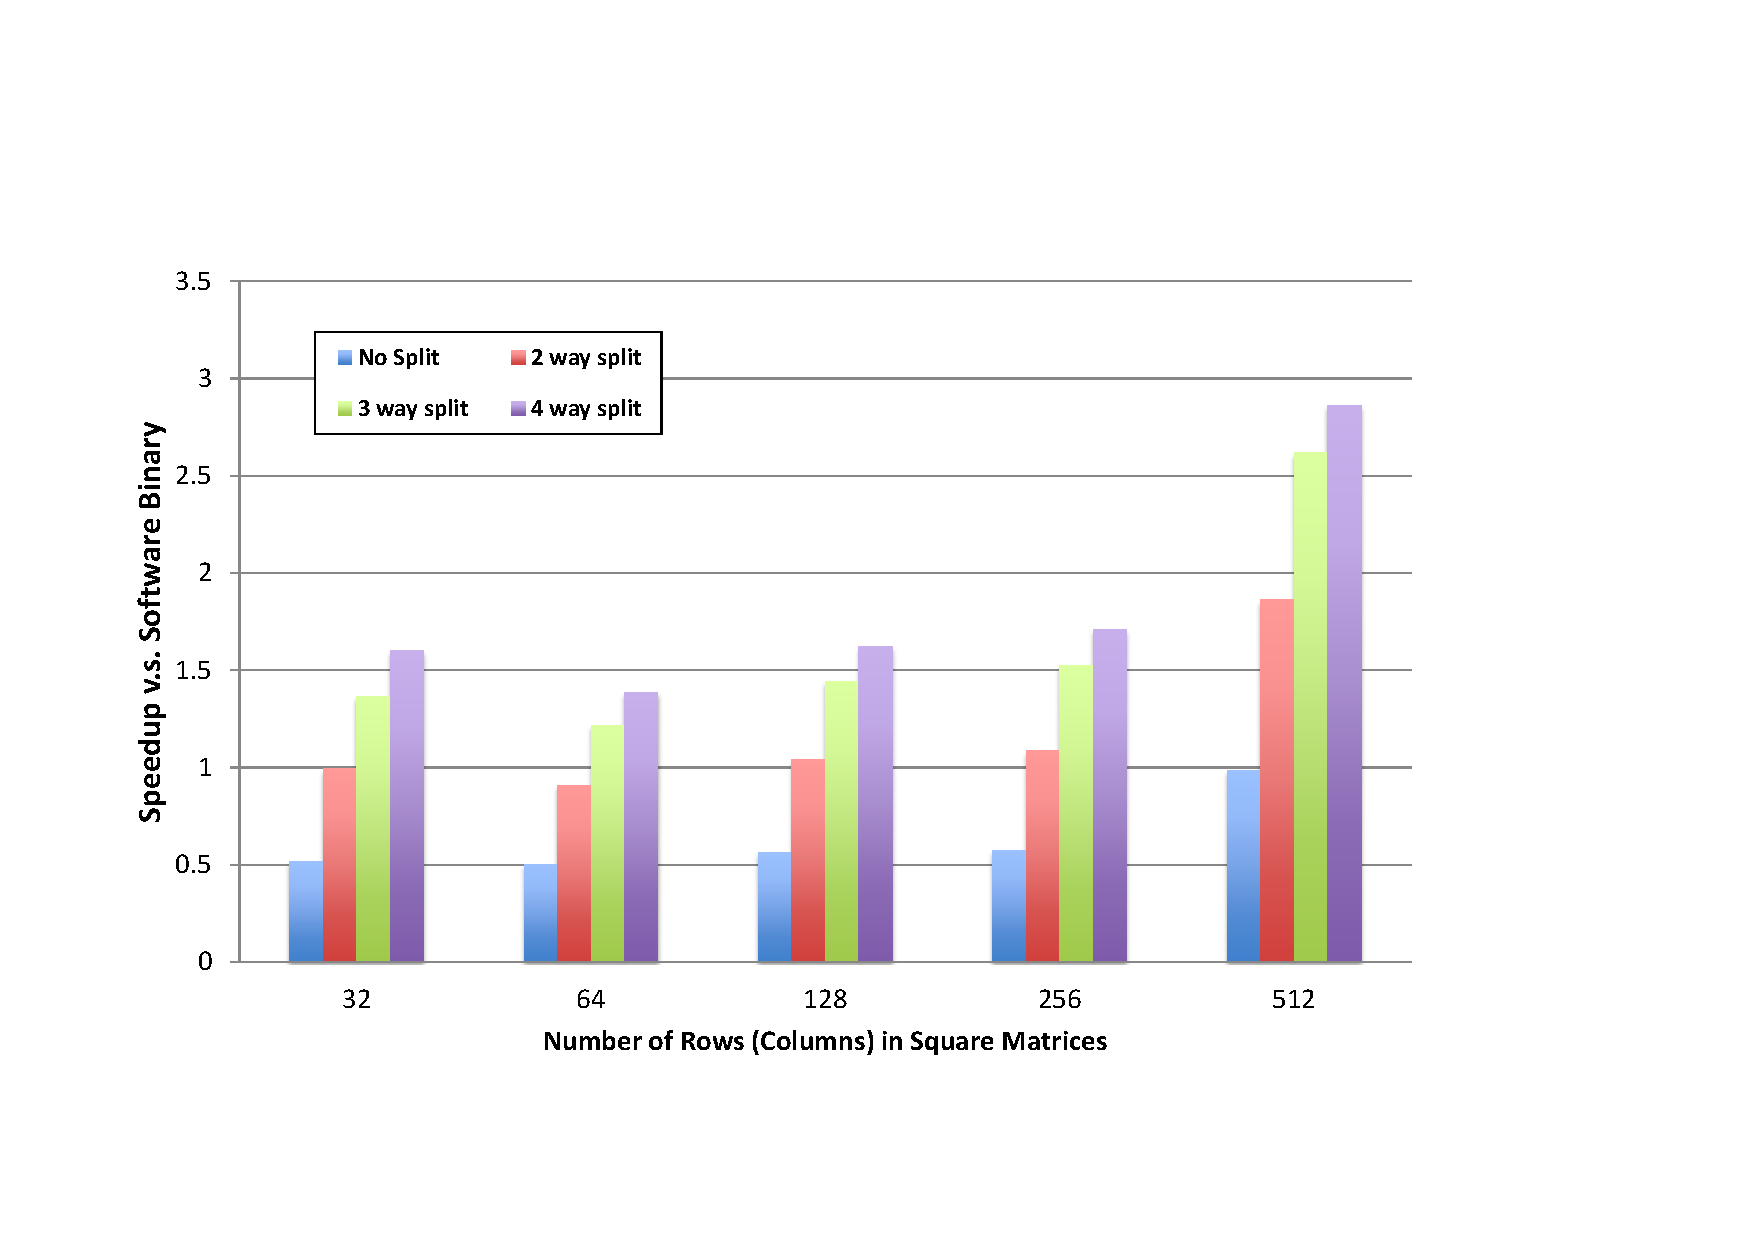
\includegraphics[width=1.0\linewidth]{chap6fig/mmultPerfSinglePort.pdf}
\caption{Performance Comparison of Decoupled Computational Pipeline and Software Binary for Matrix Multiplication
\label{fig:mmPerf}}
\end{center}
\end{figure}

Shown in figure~\ref{fig:mmPerf} is the performance as we vary the amount of iteration space splitting. As more coarse grained parallelism is exploited, the performance improves. In fact, without splitting the iteration space, the accelerator may run slower than the processor, especially when the problem size is small and fits in the CPU's cache completely. When the outer loop is splitted four ways however, the accelerator is always faster and for matrices of size 512 by 512, the speedup versus software reaches 2.7x. Note the overall performance does not scale linearly when more coarse grained parallelism is exploited. This is due to the decrease of the clock frequency as the resource utilization goes up, and the single HP port's incapability to keep up with the increase in memory requests. The second effect can be seen from figure~\ref{fig:mmPorts}, which shows how the performance of the fastest accelerator configuration (4 way split) varies as more HP ports are enabled. %As no FPGA caches are instantiated to complement the accelerators, all the memory requests are streamed directly to the HP ports. 
%Figure~\ref{fig:mmPorts} shows how the performance of the fastest accelerator configuration (4 way split) varies when more HP ports are enabled. 
In particular, there is a significant increase in performance when the the number of HP ports changes from 1 to 2, though enabling more ports beyond 2 seems to produce less pronounced effects. 

\begin{figure}[htp]
\begin{center}
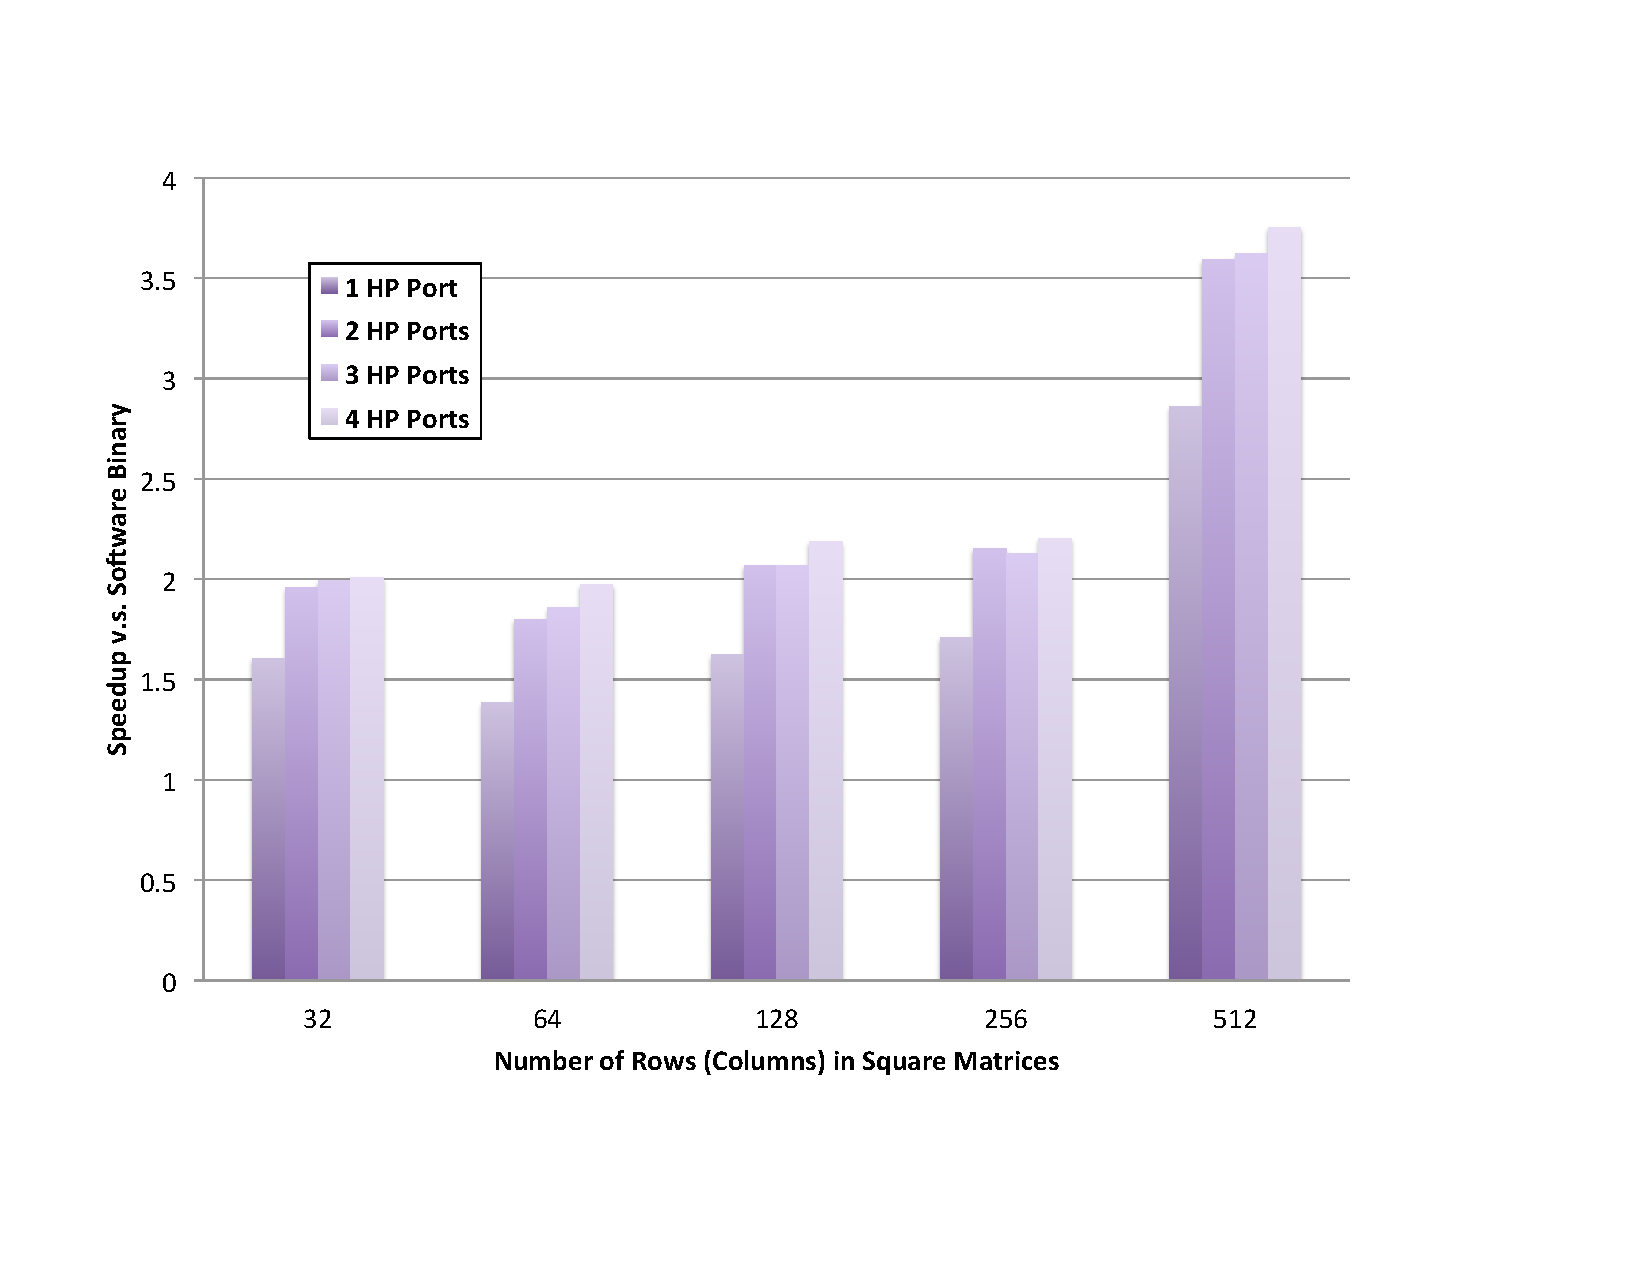
\includegraphics[width=1.0\linewidth]{chap6fig/mmPortPerf.pdf}
\caption{Matrix Multiplication Performance with 4-Way Split of the Iteration Space and Different Number of HP Ports
\label{fig:mmPorts}}
\end{center}
\end{figure}


\begin{figure}[htp]
\begin{center}
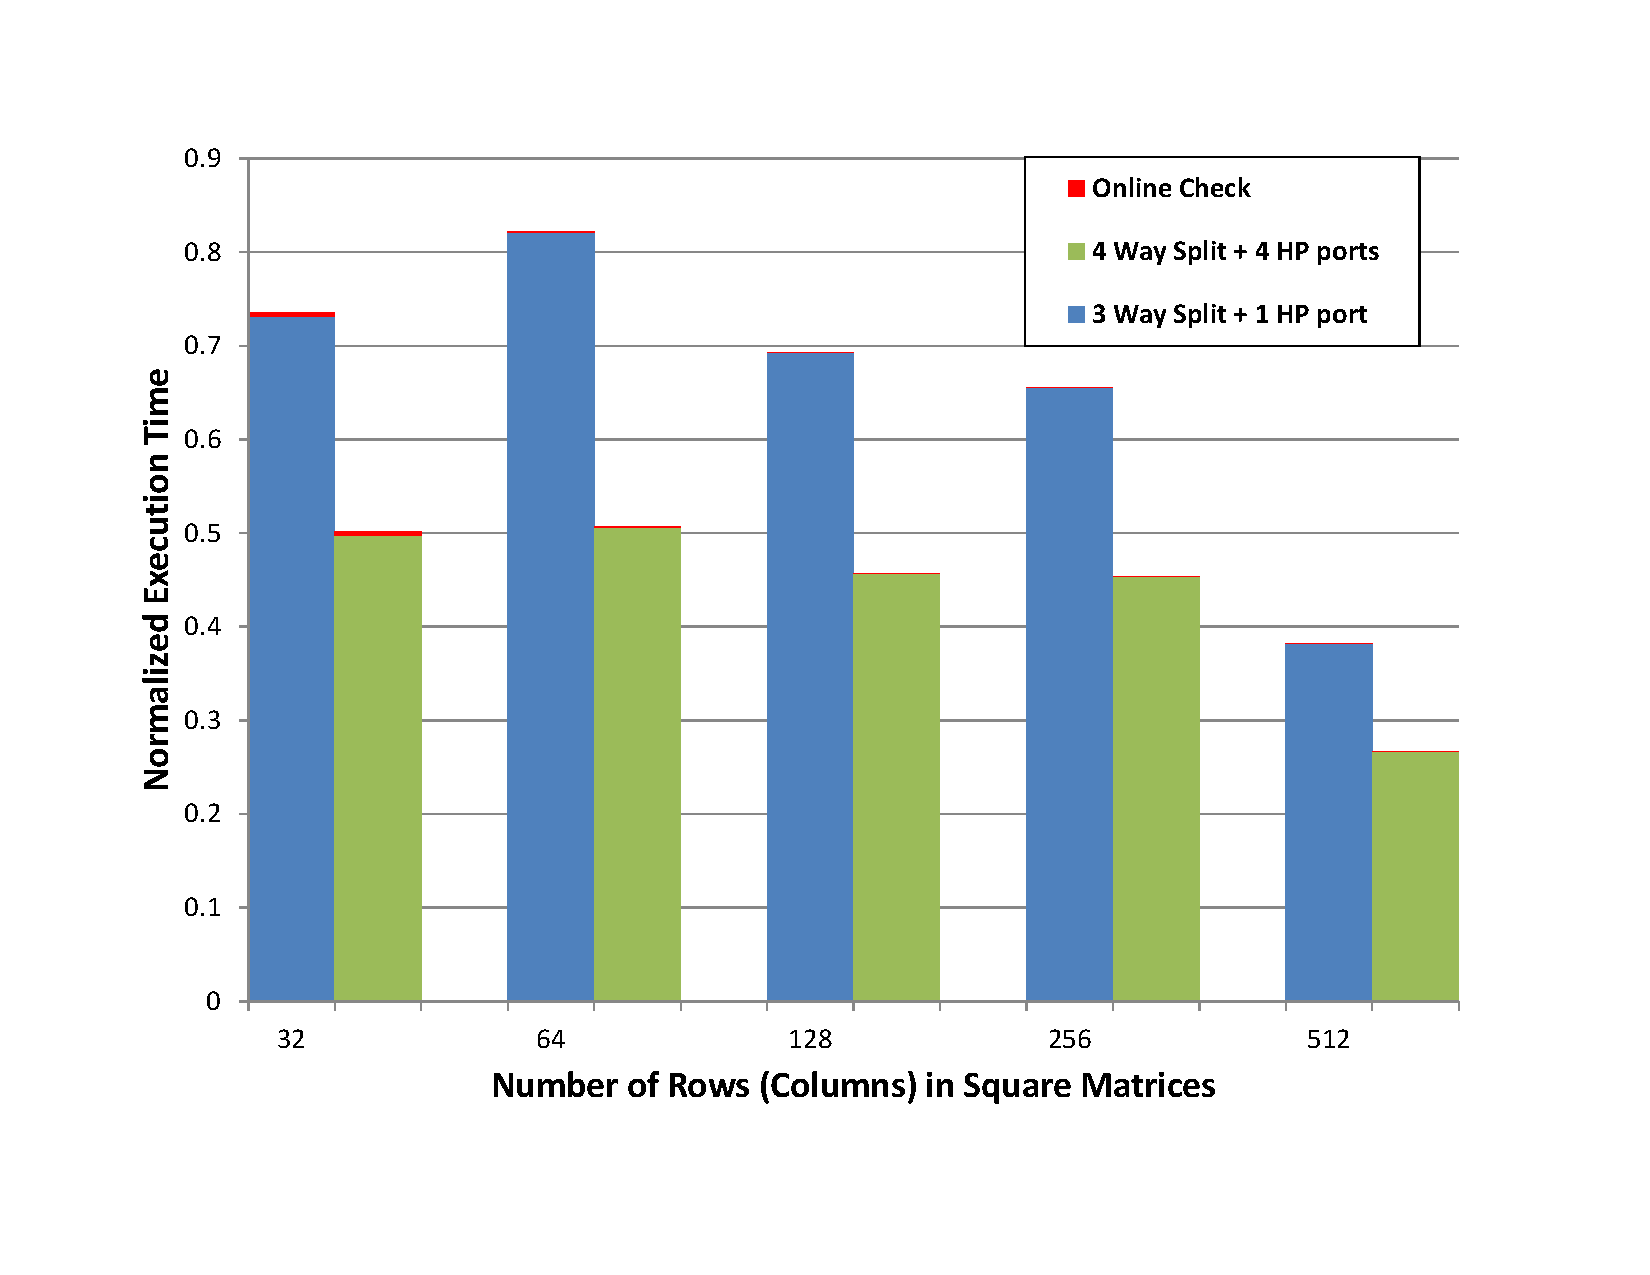
\includegraphics[width=1.0\linewidth]{chap6fig/mm2Phase.pdf}
\caption{Overall Execution Time of Accelerators with Online Checks for Matrix Multiplication
\label{fig:mmoverhead}}
\end{center}
\end{figure}

In figure~\ref{fig:mmoverhead}, the effect of online checks is shown. The actual overhead is smaller compared to the previous benchmark as the number of memory access pairs going through the test is
much smaller. 
The performance improvement provided by the two accelerator configurations listed is
virtually unaffected as the actual computation takes up two orders of magnitude more time than the dependency tests. 





\subsubsection{Benchmark 3: Sobel Edge Detection}
Another application we have benchmarked is the Sobel edge detection. An input image stored in an 2D array is convolved with small sized kernels, the result of which gets dumped into
a separate 2D array. The image can be large and may not fit on chip while a cache instantiated with programmable logic can easily buffer the kernel array.
The main loop nest extracted (convolution) in this benchmark is also a core computation pattern being used in digital signal processing, machine learning and many other fields. 

As the memory accesses in this application exhibits very high spatial and temporal locality, caches are instantiated on the programmable logic. The iteration space is again split at the outermost loop level, chunks of the input image are thus convolved with the kernel in parallel. The performance improvement over the software implementation is shown in figure~\ref{fig:convperf}.



\begin{figure}[htp]
\begin{center}
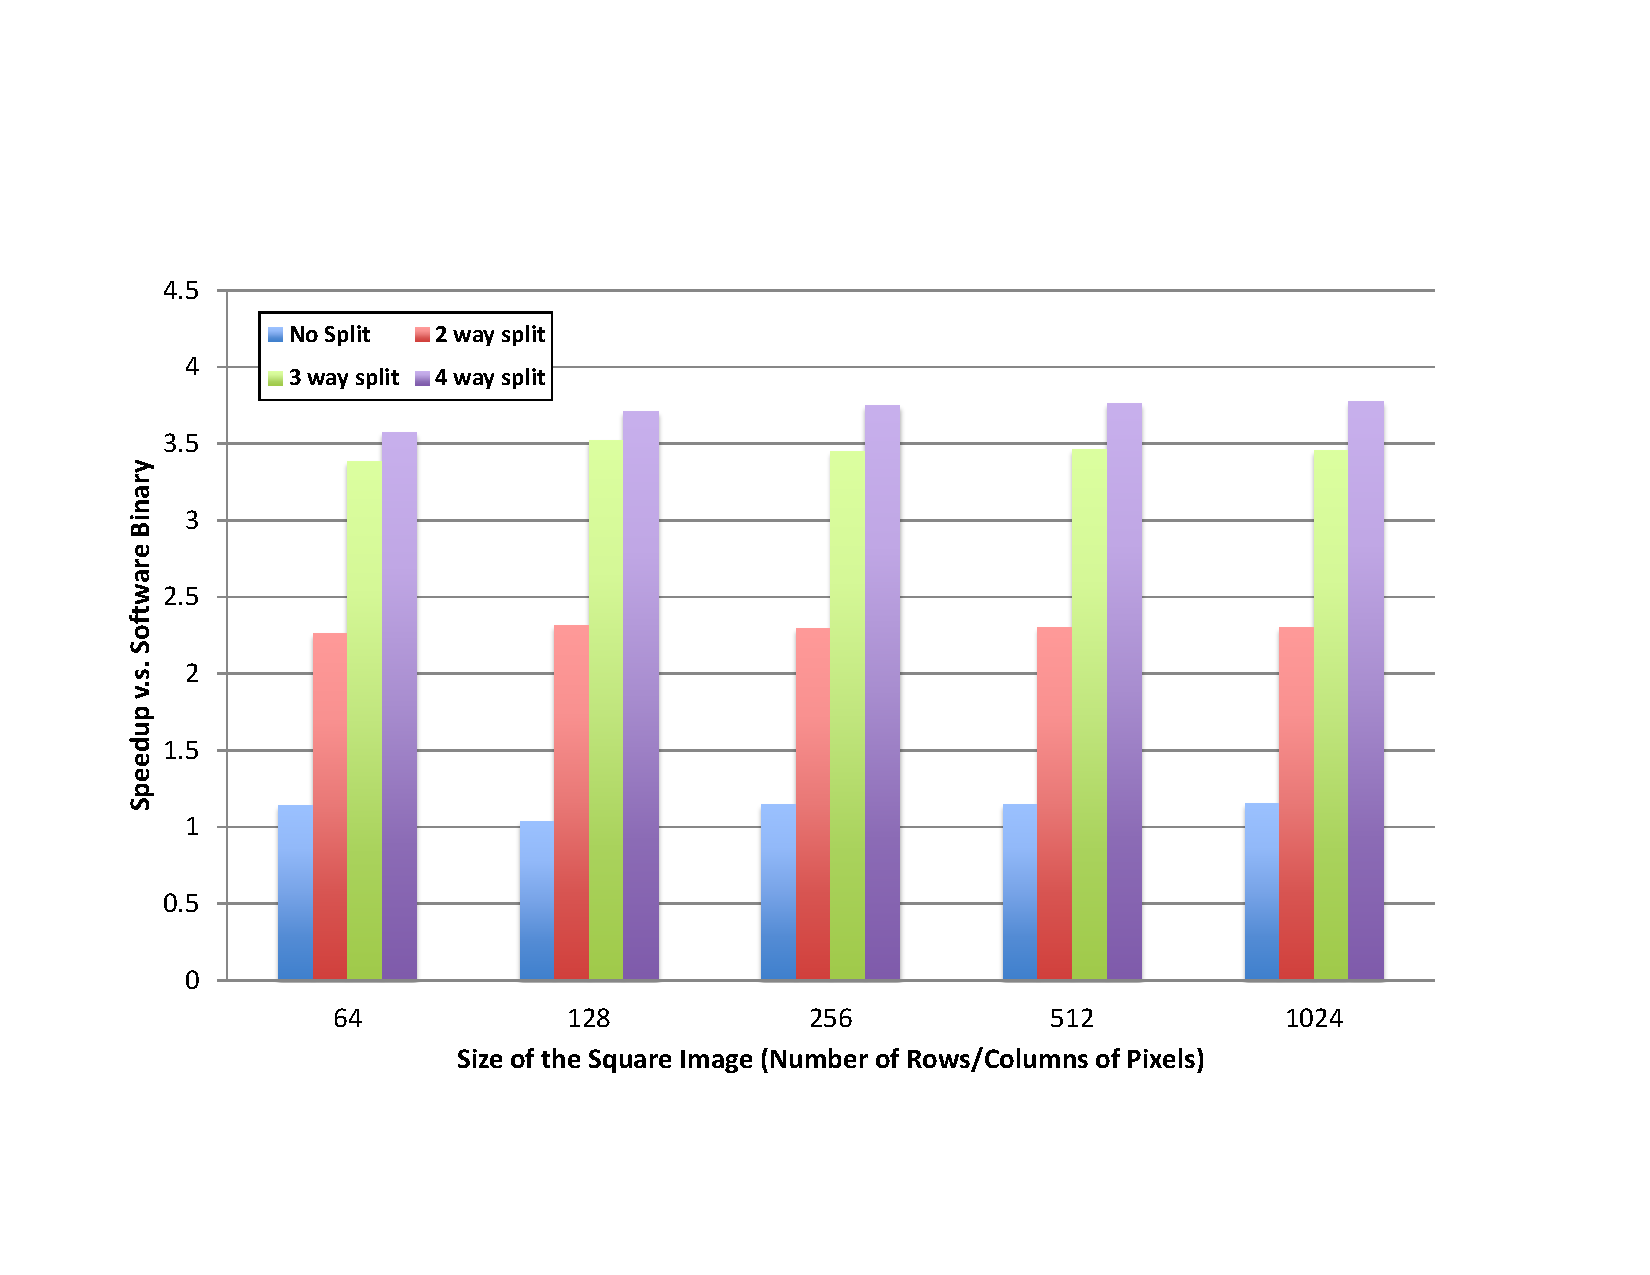
\includegraphics[width=1.0\linewidth]{chap6fig/convperf.pdf}
\caption{Performance Comparison of Decoupled Computational Pipeline and Software Binary for Edge Detection
\label{fig:convperf}}
\end{center}
\end{figure}

The speed improvement again does not scale up linearly when more
aggressive thread level parallelization is employed. The achieved clock frequency drops from 111 MHz to 91 MHz when the iteration is split four ways, which seems to account for the plateauing of performance gain completely. Figure~\ref{fig:convPorts} confirms that by showing  how enabling more ports into the memory has little effect on the performance. The caches absorbs most of the requests due to the locality of memory accesses. A single HP port is therefore sufficient for supplying data to the parallel computational pipeline.

\begin{figure}[htp]
\begin{center}
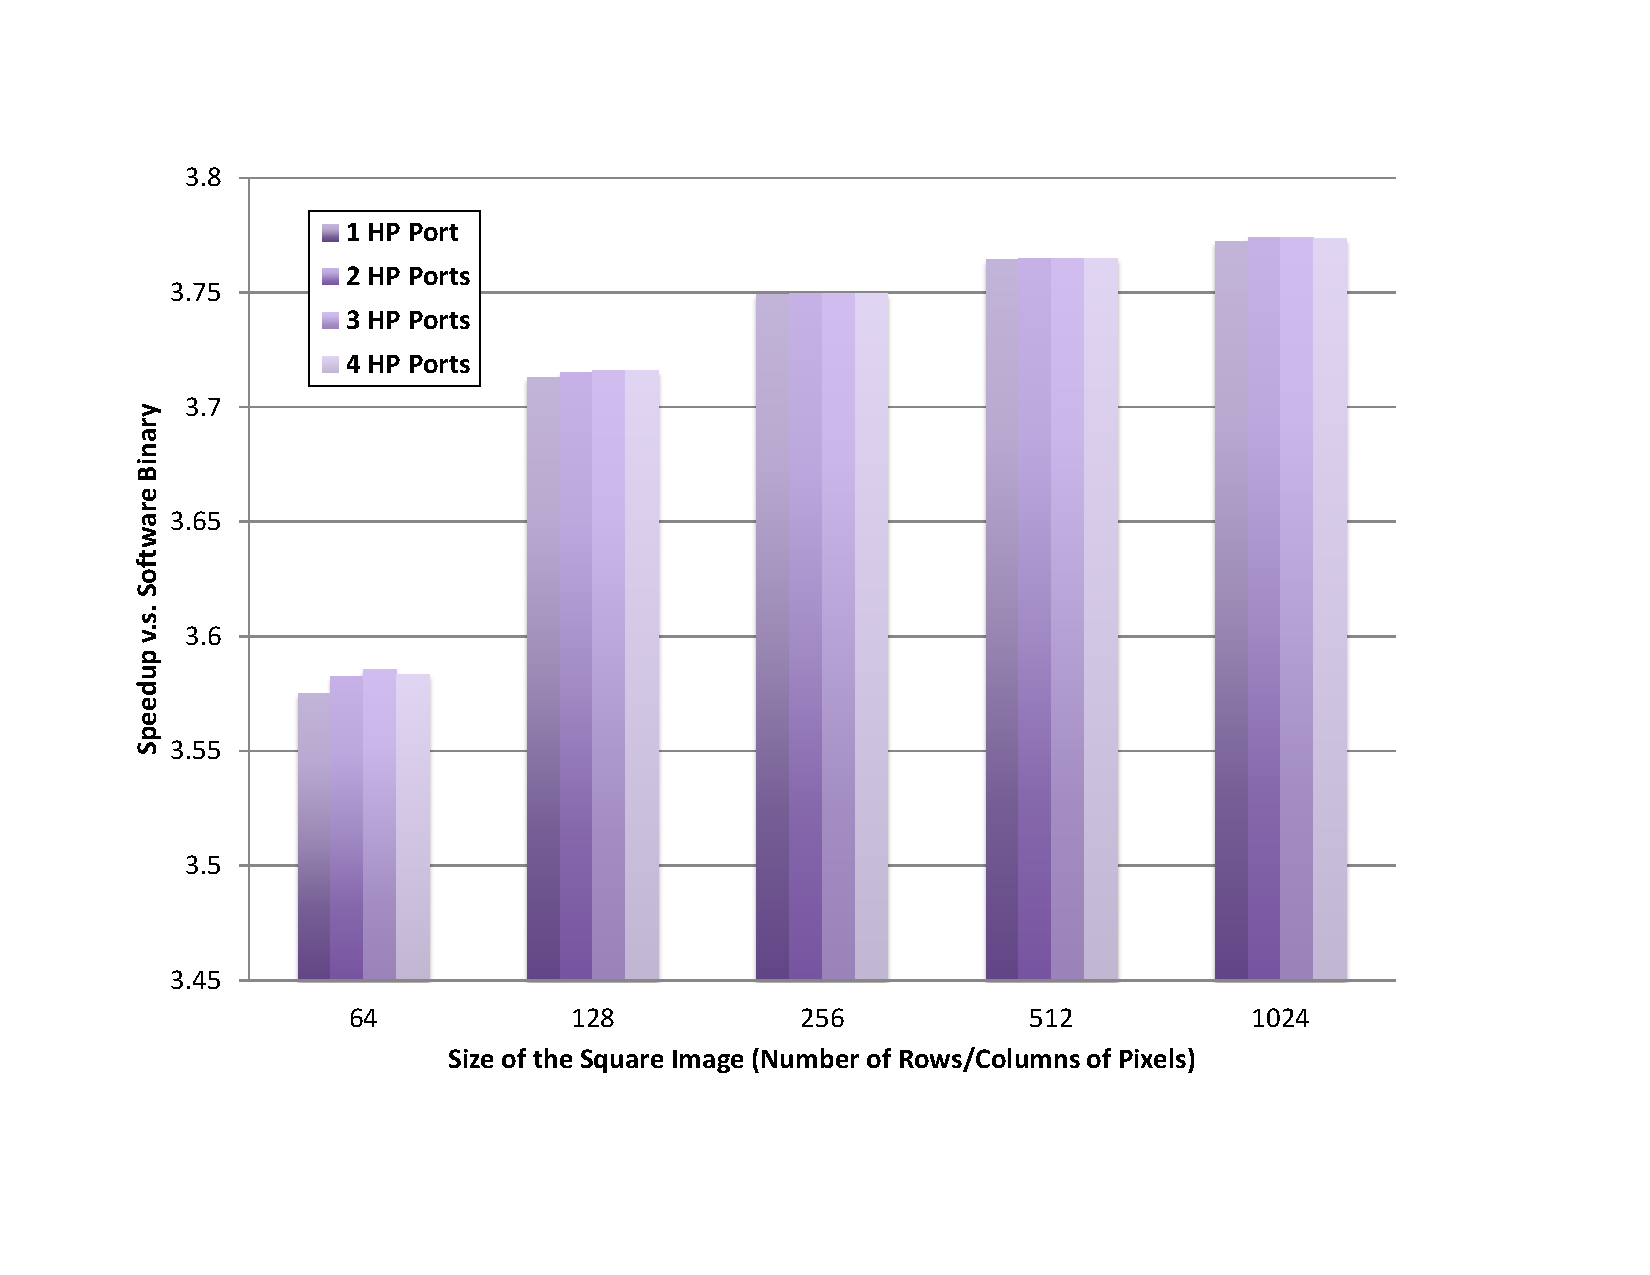
\includegraphics[width=1.0\linewidth]{chap6fig/convPortPerf.pdf}
\caption{Edge Detection Performance with 4-Way Split of the Iteration Space and Different Number of HP Ports
\label{fig:convPorts}}
\end{center}
\end{figure}

Finally, the online checks' overhead for edge detection is shown in figure~\ref{fig:conv2Phase}. Similar to previous benchmarks, the improvement provided the accelerator is not offset by the extra computation of performed before its invocation.

\begin{figure}[htp]
\begin{center}
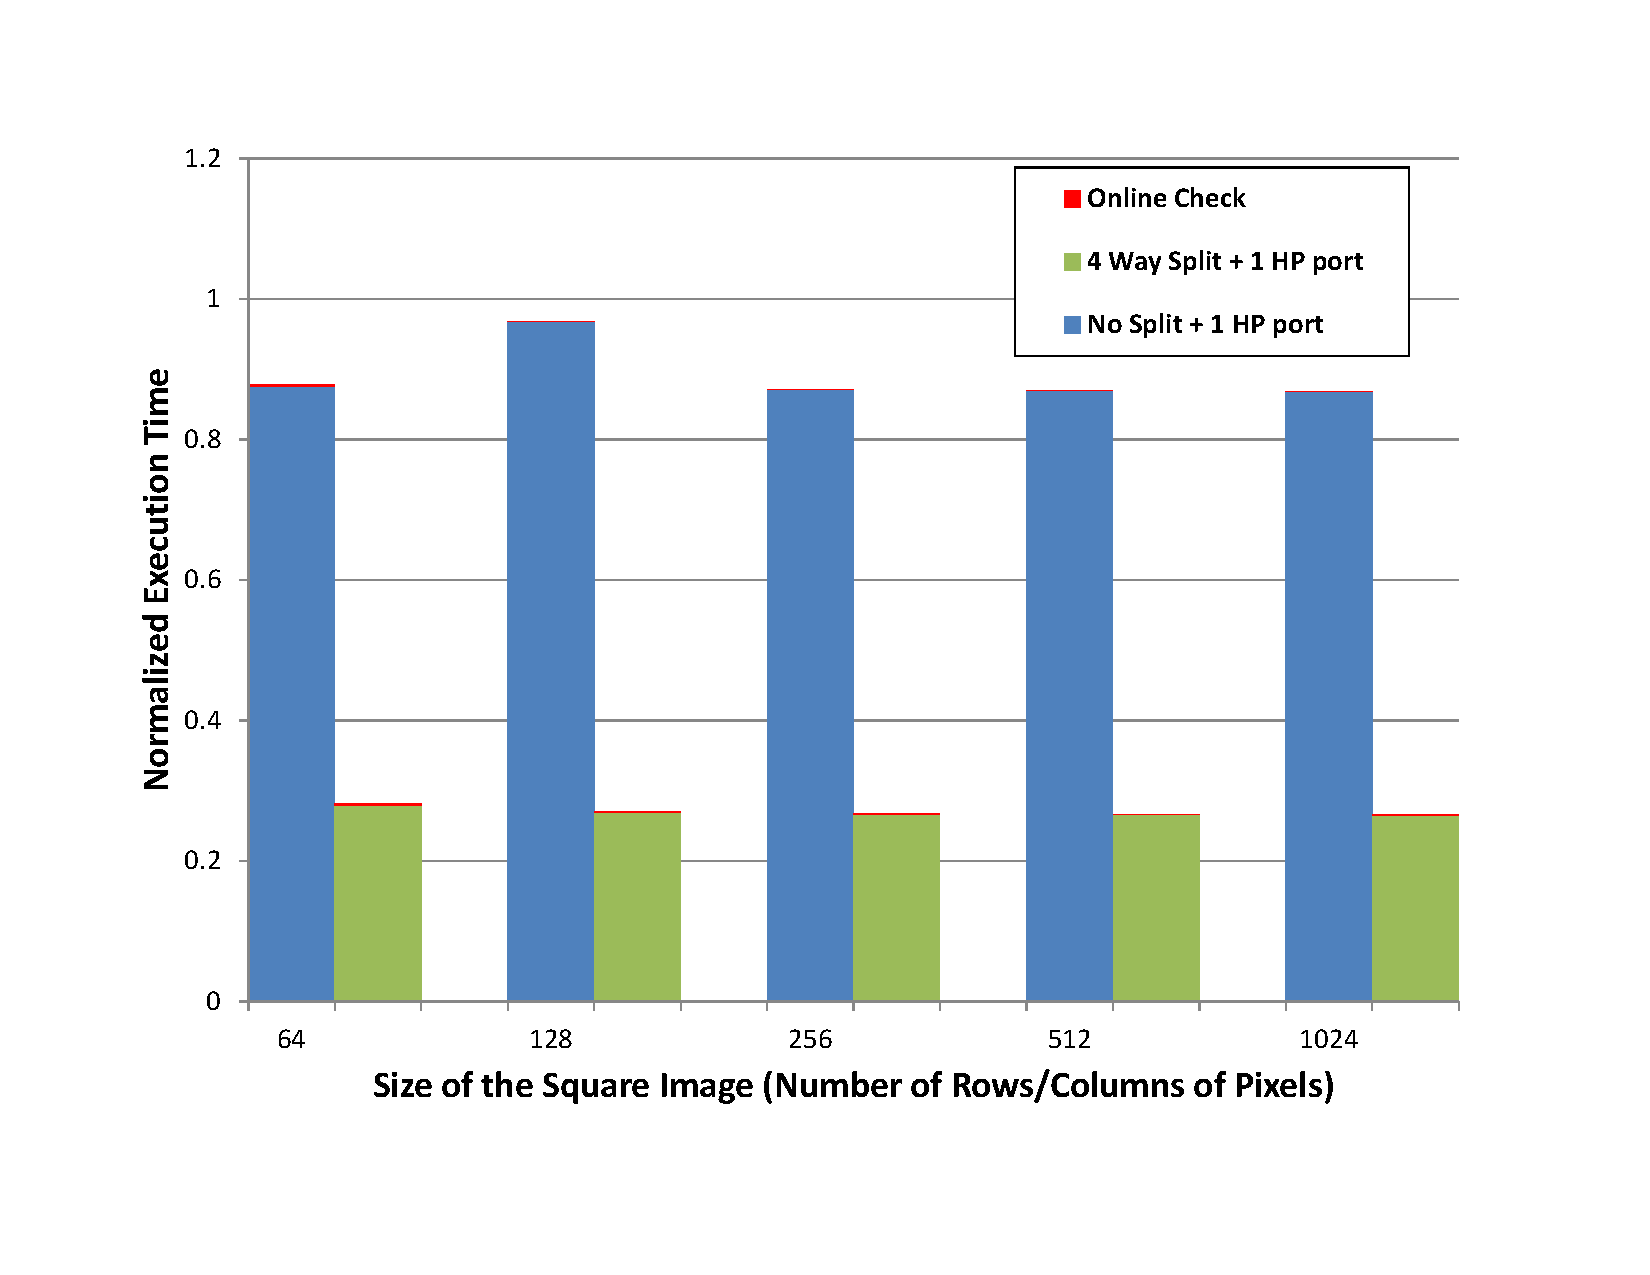
\includegraphics[width=1.0\linewidth]{chap6fig/conv2phase.pdf}
\caption{Overall Execution Time of Accelerators with Online Checks for Edge Detection
\label{fig:conv2Phase}}
\end{center}
\end{figure}




\subsection{Area Results}
Table~\ref{tab:accresults} lists how the resource usage varies with the amount of coarse grained parallelism utilized in each benchmarks. For all the benchmarks, the LUT and FF usage roughly scale linearly with
the amount of coarse grained parallelism exploited in the implementation. DSP usage in matrix multiplication, on the other hand, increases super linearly as the iteration space gets divided. This is due to the fact that in the non-multithreaded implementation, the zeroes in the lower loop bounds make it possible to generate all memory addresses without using DSP blocks. Subsequent iteration space splitting creates lower loop bounds which are run time variables, which leads to the instantiation of multipliers in the address calculation parts of the dataflow, demanding more DSP blocks. Meanwhile, GemsFDTD more than doubled its BRAM usage when two parallel threads are used. This non-linear increase did not come from the pipeline itself, but the AXI crossbars used to connect it with the HP port. As the number of memory ports exceeds 16 when two way split is performed, an additional AXI interconnect IP was instantiated, which uses a few extra BRAM blocks.

\begin{table}[htbp]
\caption{Resource Usage for Different Configurations of Decoupled Computational Pipeline}
\centering
\begin{tabular}{|c| c | c | c | c | c |}
\hline
\multirow{2}{*}{Benchmark}     &\multirow{2}{*}{}Iter. Space   &   \multirow{2}{*}{LUT} & \multirow{2}{*}{FF} & \multirow{2}{*}{DSP}& \multirow{2}{*}{BRAM}\\
 &Split & & & &\\



\hline
\hline
\multirow{2}{*}{GemsFDTD} & No Split& 19044&20209 &48 &20\\
\cline{2-6}
 & 2 Way & 38730 & 41749&96 &45\\
\hline
\multirow{3}{*}{} & No Split& 9441 &7945 &5 &6\\
\cline{2-6}
 Matrix& 2 Way  & 18505 &16772 &14 &12\\
 \cline{2-6}
 Multiplication& 4 Way  & 36488 &30254 &32 &24\\
\hline
\multirow{3}{*}{} & No Split& 12184 &13413 &27 &30\\
\cline{2-6}
 Sobel Edge& 2 Way  & 22879 &25433 &54 &61\\
 \cline{2-6}
 Detection& 4 Way  & 43500 &49001 &108 &122\\
\hline

\end{tabular}
\label{tab:accresults}
\end{table}


Overall, for each loop nest, which accelerator configuration to use depends on if the area used is justifiable in light of the other accelerators' potential to provide speedup. As we are
only exploring the possibility of binary based accelerator generation by looking at a single loop nest at a time, the investigation of this trade-off is left to future work.

\begin{comment}
\begin{table}[htbp]
\caption{Input Data Set for the Benchmarks}
\centering
\begin{tabular}{| c | c | c | }
  \hline            
  
 \multirow{2}{*}{Benchmark}   &   \multirow{2}{*}{Description of Input Data} & \multirow{2}{*}{Total Size of Input Data}\\
 &       &   \\
  \hline            
  \hline            
\multirow{2}{*}{}Gems&  Matrix dimension = 4096 & \multirow{2}{*}{ $\approx$ 16 MB}  \\
%\cline{2-3}                                                                                                                                                    
 FDTD &Density of Matrix = 0.25       &  \\
%\cline{2-3}                                                                                                             
   \hline                                                                                                           
\multirow{2}{*}{}Sobel&  Weight Limit = 3200 &\multirow{2}{*}{$\approx$ 5 MB}  \\
%\cline{2-3}                                                                                                                                                    
 Edge Detection &Number of Items = 200       &   \\
%\cline{2-3}                                                                                                             
\hline
\multirow{2}{*}{}Matrix& \multirow{2}{*}{Number of Nodes = 1024}  & \multirow{2}{*}{$\approx$ 8 MB}  \\
%\cline{2-3}                                                                                                                                                    
 Multiplication &       &   \\
%\cline{2-3}                                                                                                                                                        
  \hline                                                                                                           
\end{tabular}
\label{tab:kerSize}
\end{table}

Size of the dataset for each benchmark is summarized in table~\ref{tab:kerSize}. We have taken advantage of the memory level parallelism to generate multiple data access interfaces on the datapath side. The complementary hardware structure connecting to the memory subsystem is also customized, using optimizations described in  section~\ref{customDataAccess}.
\end{comment}

%as the memory access pattern varies

%the datapath's connection with the memory subsystem is also
%customized, similar to the 


%\subsection{Overhead of Runtime Checks}










\section{Discussion and Future Work}

\subsection{Application of Our Approach in Other Contexts}
Our two phased approach leveraging both the run time profile and the static program 
can be used for parallelization in other contexts as well. There are certain functions
whose memory access patterns are not necessarily analyzable using only the source code. An example of this is shown in figure~\ref{fig:srcAna}. As the data structures
are passed into the function using pointers, the constant terms (a, b and c) and the coefficient (dim) in the Diophantine equations are all unknown. Banerjee's method, in this case, does not produce affirmative result. On the other hand, with the help of runtime profile,  this function can also be analyzed. In this example, as negative results are produced when tested for the dependency vector (*,*), every level of the loop is parallelizable. 
\begin{figure}[htp]
\begin{center}
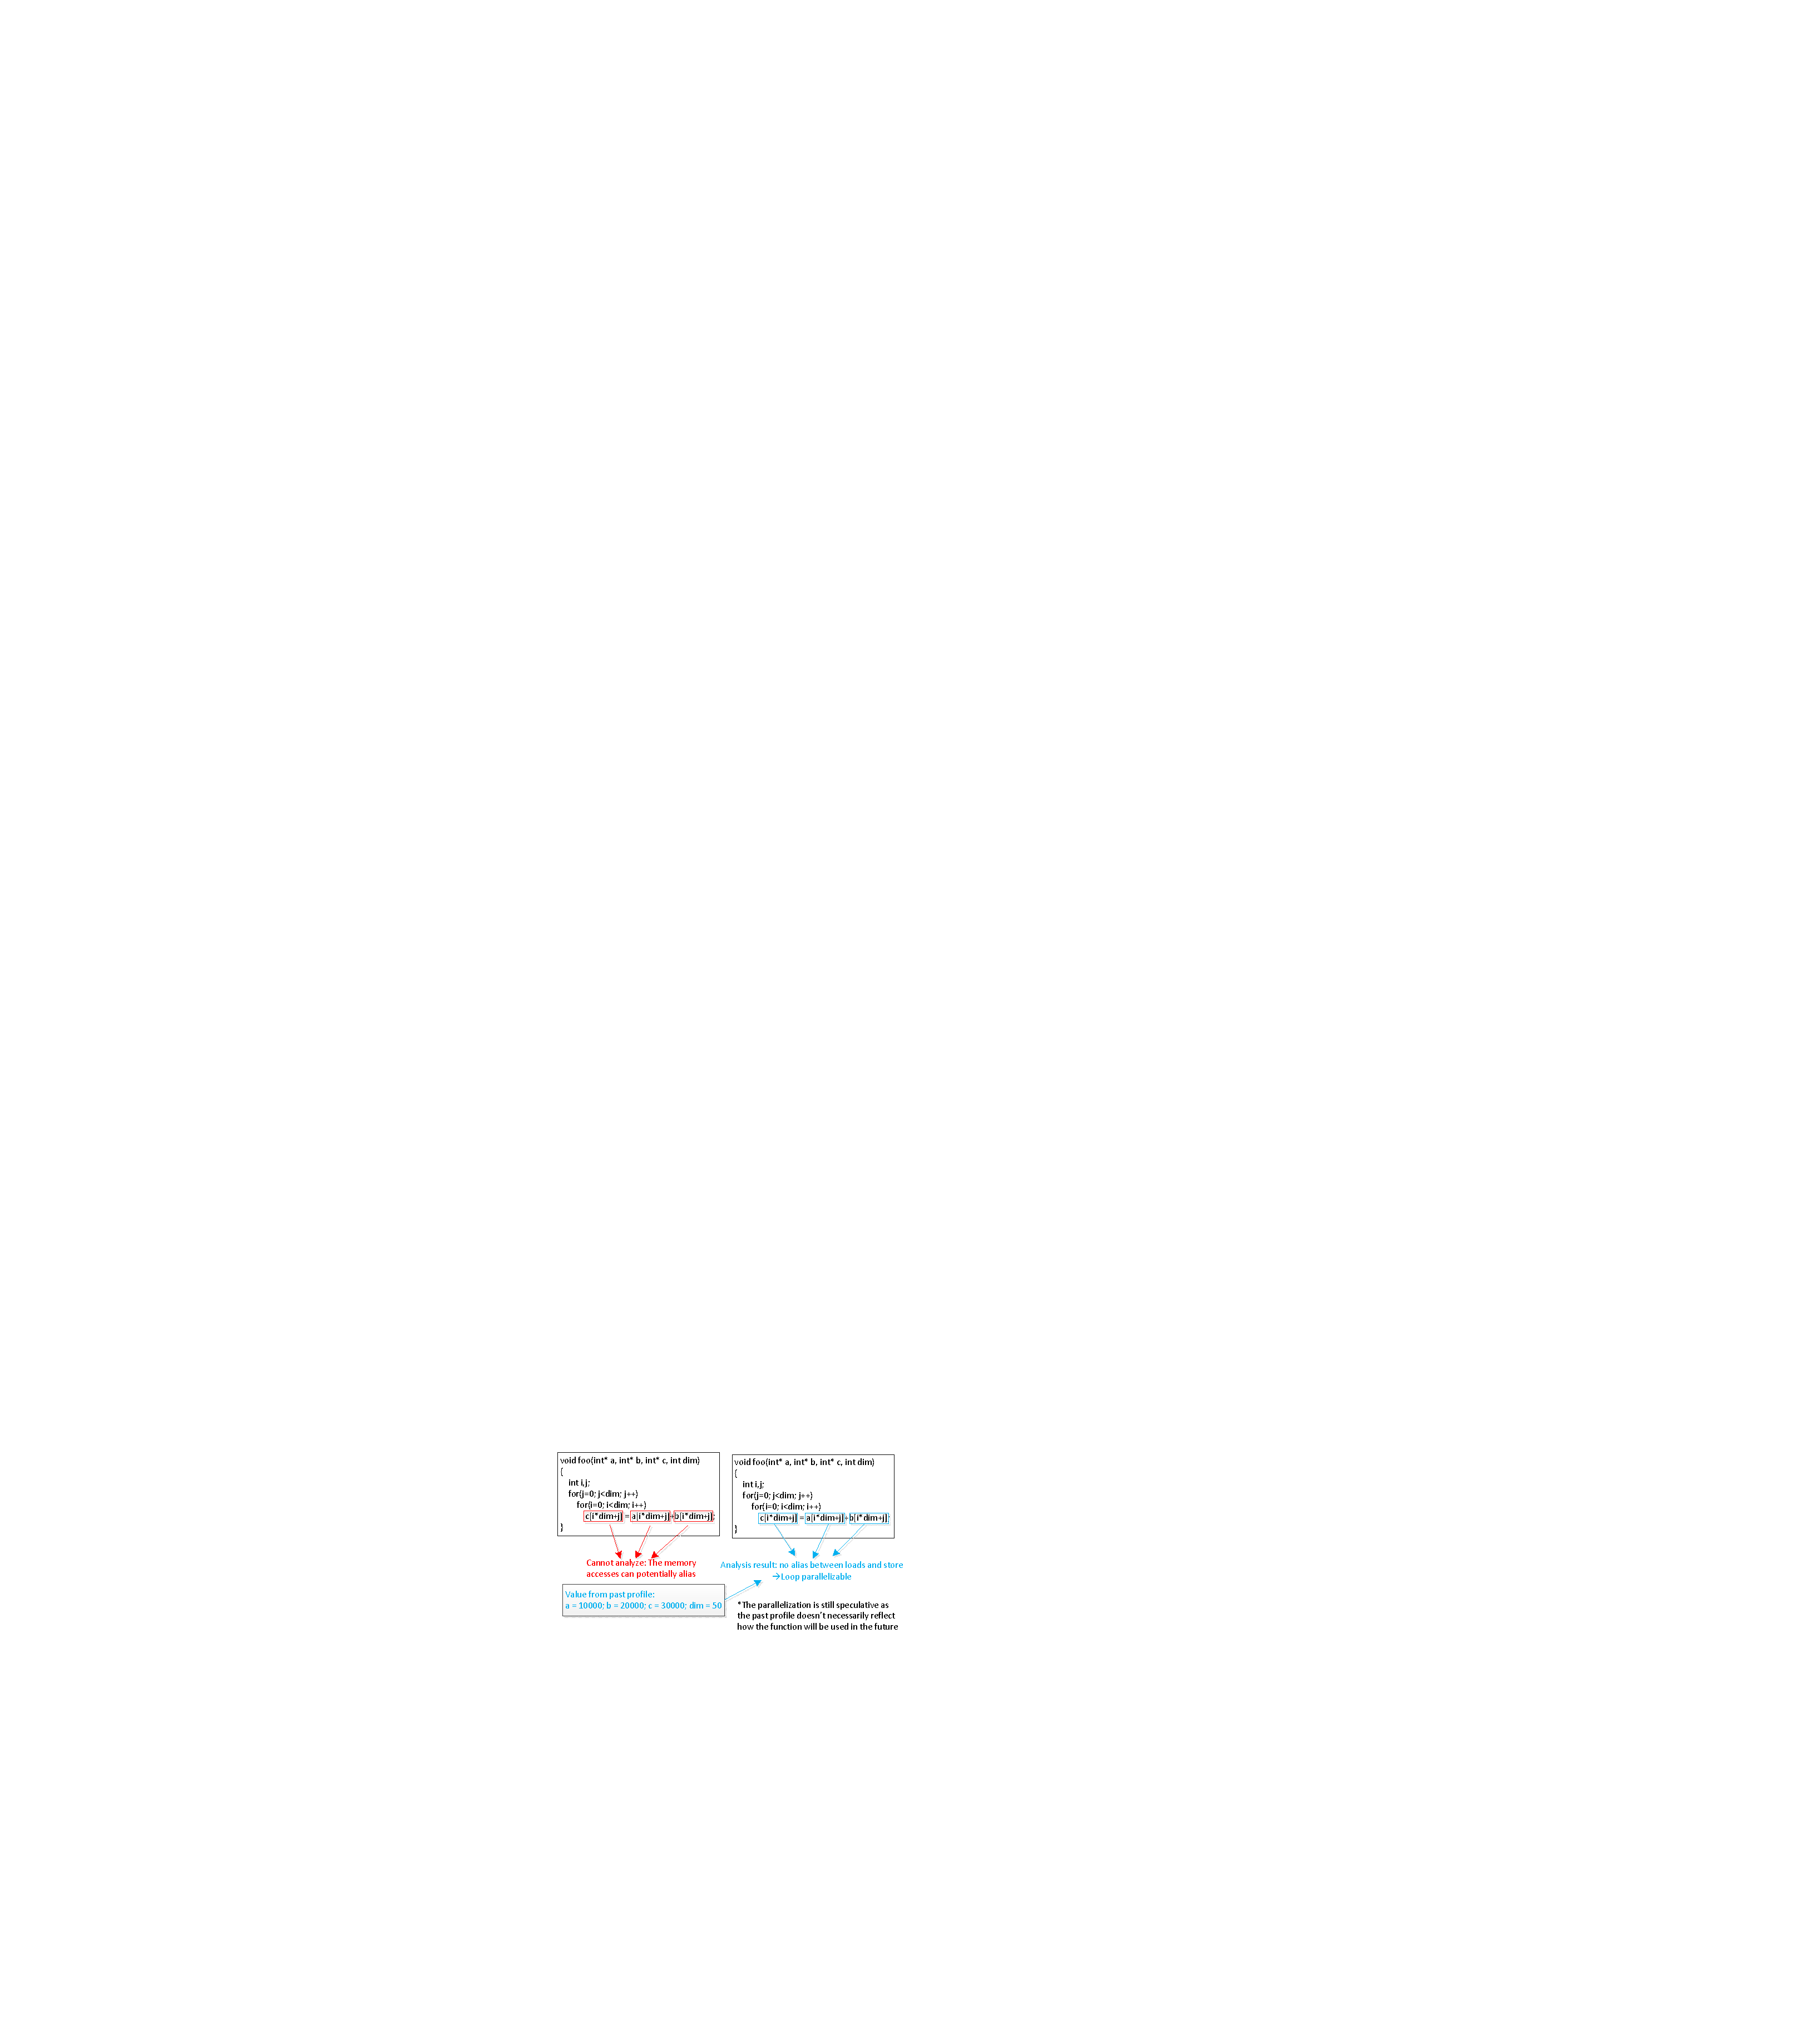
\includegraphics[width=0.85\linewidth]{chap6fig/sourceCodeAnalysis.pdf}
\caption{Analyze Loop in C with Value from Past Profile 
\label{fig:srcAna}}
\end{center}
\end{figure}

Other parallel compute platforms can also be the targets of our methodology. Depending on the speed of the compilation toolchain, the $offline$ phase may potentially be performed during run time. If this online compilation uses the current run time profile, we can forgo the additional online checks and essentially have just-in-time parallelization. In general the choice between having a cached parallel implementation with online checks and performing just-in-time parallelization largely hinges on the speed with which parallel implementation can be created, relative to the execution time of the original code. FPGA accelerators, with potentially hours of compilation time, falls on one end of this spectrum and the two phased approach ends up being the most appropriate one.



\subsection{Data Transfer for CPU-FPGA system with Separate Address Space}
\label{dtransfer}

%comment out tmep
%\subsubsection{Communication between CPU and FPGA Memory Spaces}
%Another particular important aspect in ensuring the efficient execution of the accelerators is in the management of data transfers. 
As the FPGA is used to implement accelerators for %binaries 
programs executed on CPU, both the source
and final destination of its working datasets are the address space of
the processor. Our framework assumes the FPGA can directly access the CPU's memory, and leverages the decoupled computational pipeline synthesis flow to naturally extract sets of address generators who stream requests
into the memory subsystem. 
%Depending on the actual configuration of the system, the processor memory may or may not be directly accessible by the FPGA, as discussed in section~\ref{chartarg}. We thus need to provide mechanisms to enable the sharing of data between the two substrates.
%
%
%For the cases where the FPGA can directly access the CPU's address space, which are the targets for our flow, the transformation and optimizations described in chapter~\ref{decoupleChap}, would naturally create a set of address generators who pipeline requests into the memory subsystem, as can be seen from figure~\ref{show3demuPipeline}. 
%To benefit from the locality-driven optimization we have performed, 
%Caches can also be inserted between the address outputs and the
%off-chip memory to take advantage of the any potential data locality.
%
\begin{comment}
\begin{figure}[htp]
\begin{center}
\includegraphics[width=0.5\linewidth]{chap6fig/pipelineAddressGen.pdf}
\caption{Address Generators and Compute Modules in the Generated Decoupled Computational Pipeline
\label{show3demuPipeline}}
\end{center}
\end{figure}
\end{comment}
%
On the other hand, %In a more complex scenario, 
in systems where the FPGA has its own address space, 
%into which 
the program data would need to be explicitly transferred into and out of it before and after the accelerator execution. %can occur. The output from the accelerator is also moved explicitly back to the host CPU's address space.
%and a hardware module accessing the CPU memory directly in master mode is implementable. 
Many of the state-of-the-art platforms with this model
are connected to the host through PCI-e connections, which is rather similar to discrete GPU platforms.
As the GPGPUs were getting more widely adopted, the automatic management of their communication with the CPU hosts was also studied in multiple projects~\cite{Pai:2012:FEA:2370816.2370824}\cite{Jablin:2011:ACC:1993316.1993516}\cite{Jablin:2012:DMD:2259016.2259038}. Most of these frameworks require compiler assistance or user guidance to facilitate the management of data transfers and is therefore not directly applicable to a flow targeting existing program binaries. 

For the case where the offloaded computation is assumed to have analyzable memory access patterns, like in our flow, it is possible to calculate \textit{a priori} the  memory footprint for the accelerated loop nests. 
As the referenced addresses are always affine functions of the loop indices, for a given part of the iteration space, the boundaries of the accessed range of memory by an instruction can always be
computed. This computation would become another part of the $online$ $phase$, supplying parameters for the actual data movement mechanisms. 

There is certainly a large space for exploration when it comes to performing the data transfer, especially when the addresses referenced by the loop nest are non-contiguous. 
%Depending on the memory access pattern of the accelerated loop nest, the schedule with which data gets copied to the
%FPGA memory may have significant effect on the final performance. 
Many fine grained data transfers may be less efficient compared
to a few coarser grained memcpy invocation, even though the later may incur wastage as some unused data is also moved. 
Co-optimizing the data transfer and the computation parallelization based on application specific memory access patterns requires significant effort and can
be an interesting direction for future research.  


%Meanwhile, overlapping the copying operation with the on-FPGA computation can help boost the overall performance. 
% With the data finally resident in the FPGA's address space, every original access can be translated to a memory reference in the new context by adding/removing an offset. Depending on how the original working dataset is broken down into memory objects, this offset is computed differently.

\begin{comment}
and the two main FPGA vendors both allow for
OpenCL to be used to program some of these systems. 
Thus We would like to discuss the data transfer mechanism based on OpenCL's data communication model. 
The steps needed include: 
\begin{itemize}
    \item Compute the range of memory addresses to be transferred to and from the FPGA device
    \item Memory allocation on the target FPGA board: $clCreateBuffer$ 
    \item Data transfer to FPGA: $clEnqueueWriteBuffer$
    \item Invoke accelerator: $clEnqueueNDRangeKernel$
    \item Data transfer back to CPU address space: $clEnqueueReadBuffer$
\end{itemize} 

It is worth noting that shared virtual memory (SVM) support has been introduced in OpenCL2.0 where the data movement between the host CPU and the FPGA device can be implicitly handled by the runtime. However, even
in platforms supporting SVM, a buffer is to be allocated explicitly and populated with the appropriate data. For our binary based flow, there is still a need to perform the address range computation, memory allocation and kernel(accelerator) invocation. The difference is that now the explicit data transfer between devices gets
replaced by memcpy between the already allocated memory of the original program binary and the SVM buffer just created. 


The analyzability required for coarse grained parallelism discovery 
also enables the \textit{a priori} calculation of the  memory footprint for the accelerated loop nests. As the referenced addresses are always affine functions of the loop indices, for a given part of the iteration space, the boundaries of the accessed range of memory by an instruction can always be
computed. This computation would become another part of the $online$ $phase$, supplying parameters for the actual data movement mechanisms. 

There is certainly a large space for exploration when it comes to how to perform the data copy. Depending on the memory access pattern of the accelerated loop nest, the schedule with which data gets copied to the
FPGA memory may have significant effect on the final performance. Co-optimizing the data transfer and the computation parallelization can
be an interesting direction for future research. 

In particular, the accessed memory locations can be highly fragmented
with large gaps between them. How to schedule the movement of various piece of data may have significant effects on the final performance. The

To only move the referenced data might result in many invocations of the data copying routine. It might be beneficial to copy some extra bytes but issue less data moving commands.  


...
sparse, multiple memcpy may reduce wasted bandwidth for transfer, but increases the overhead in invocation data transfer mechanisms. Application-specific exploration



With the data finally resident in the FPGA's address space, every original access can be translated to a memory reference in the new context by adding/removing an offset. Depending on how the original working
dataset is broken down into memory objects, this offset is computed differently.
%An example is shown in  figure~\ref{a-memory-reference-get-offseted}. 
In essence, the data transfer mechanism constructs functions for mapping addresses in CPU memory to memory objects accessible by FPGAs. 
%tuples of (memory object, address) in FPGA memory space. 
The affine function mapping points in the iteration space to addresses in CPU memory gets transformed, through adding offsets, to address data
in the new device. 

%composed with these newly constructed function to 



If OpenCL is actually being used to perform hardware generation, the analysis work we have done to extract coarse grained parallelism would still work.
At the same time...packaging the transferred data into the memory objects can affect the final performance as well. Having everything in a single 
object in openCL's global memory space ------ not good, less memory level parallelism even though the data transfer between host and FPGA platform
is easier. 

Several research projects explored automatic management of memory transfers
in CPU-GPU systems~\cite{Pai:2012:FEA:2370816.2370824}\cite{}, most of which
requires compiler assistance and may not be directly applied in a flow targeting program binaries.

\end{comment}

\begin{comment}
\subsection{Address Translation}
When virtual addressing is involved, another layer of complexity is added to the communication between the hardware accelerator and the CPU's memory address space. The CPU's address translation mechanism is normally not accessed by the FPGA, whose outgoing memory requests therefore must use
physical addresses. The generation of addresses by the FPGA accelerator, however, was based off virtual addresses extracted from the software running on the CPU before the accelerator's invocation. It thus becomes necessary to map the virtual addresses generated by the hardware logic to the physical addresses used by the memory subsystem.

In the case where the CPU's memory is not accessible to FPGA
directly and explicit data movement is needed, as just described above, this is less of a problem. One part of the translation happened on the CPU side when the transfer occurs, the virtually referenced data structure get extracted and placed contiguously into the FPGA's physically addressed memory. The remaining part of the translation, as described in part~\ref{dtransfer}, is merely associating references with new memory objects and adding offsets -- a simple and inexpensive process.

On the other hand, if the FPGA is to directly generate the addresses used to access the CPU's memory, virtual to physical address translation would need to happen. As the processor's memory management unit is normally not directly accessible to the FPGA, its functionality needs to be handled using the programmable logic. Several different mechanisms have be devised in
previous projects~\cite{6718414}\cite{7459405}\cite{4042434}, some acting
as a full replacement of the MMU while others take advantage of the assumed
memory access pattern to simplify the hardware. In our case, as we have




It is particularly interesting to look at the interaction between memory level parallelization and coarse grained parallelization. The pipelining of
loops is a form of instruction reordering, in the absence of memory level
parallelism, the amount of speed up achievable is rather limited~\cite{nwcache}. Similarly, when loops are unrolled, more memory operations are exposed in every iteration of the loop. The increased hardware cost is only justifiable if there are enough simultaneous data streams from the memory subsystem to satisfy the multiplied throughput provided by the wider datapath. The same constraint is applicable to thread-level parallelization as well. For regular computation kernels we target, it is
possible to analytically estimate how much coarse grained parallelization
should be performed given a memory bandwidth budget.


\end{comment}




\begin{figure}[htp]
\begin{center}
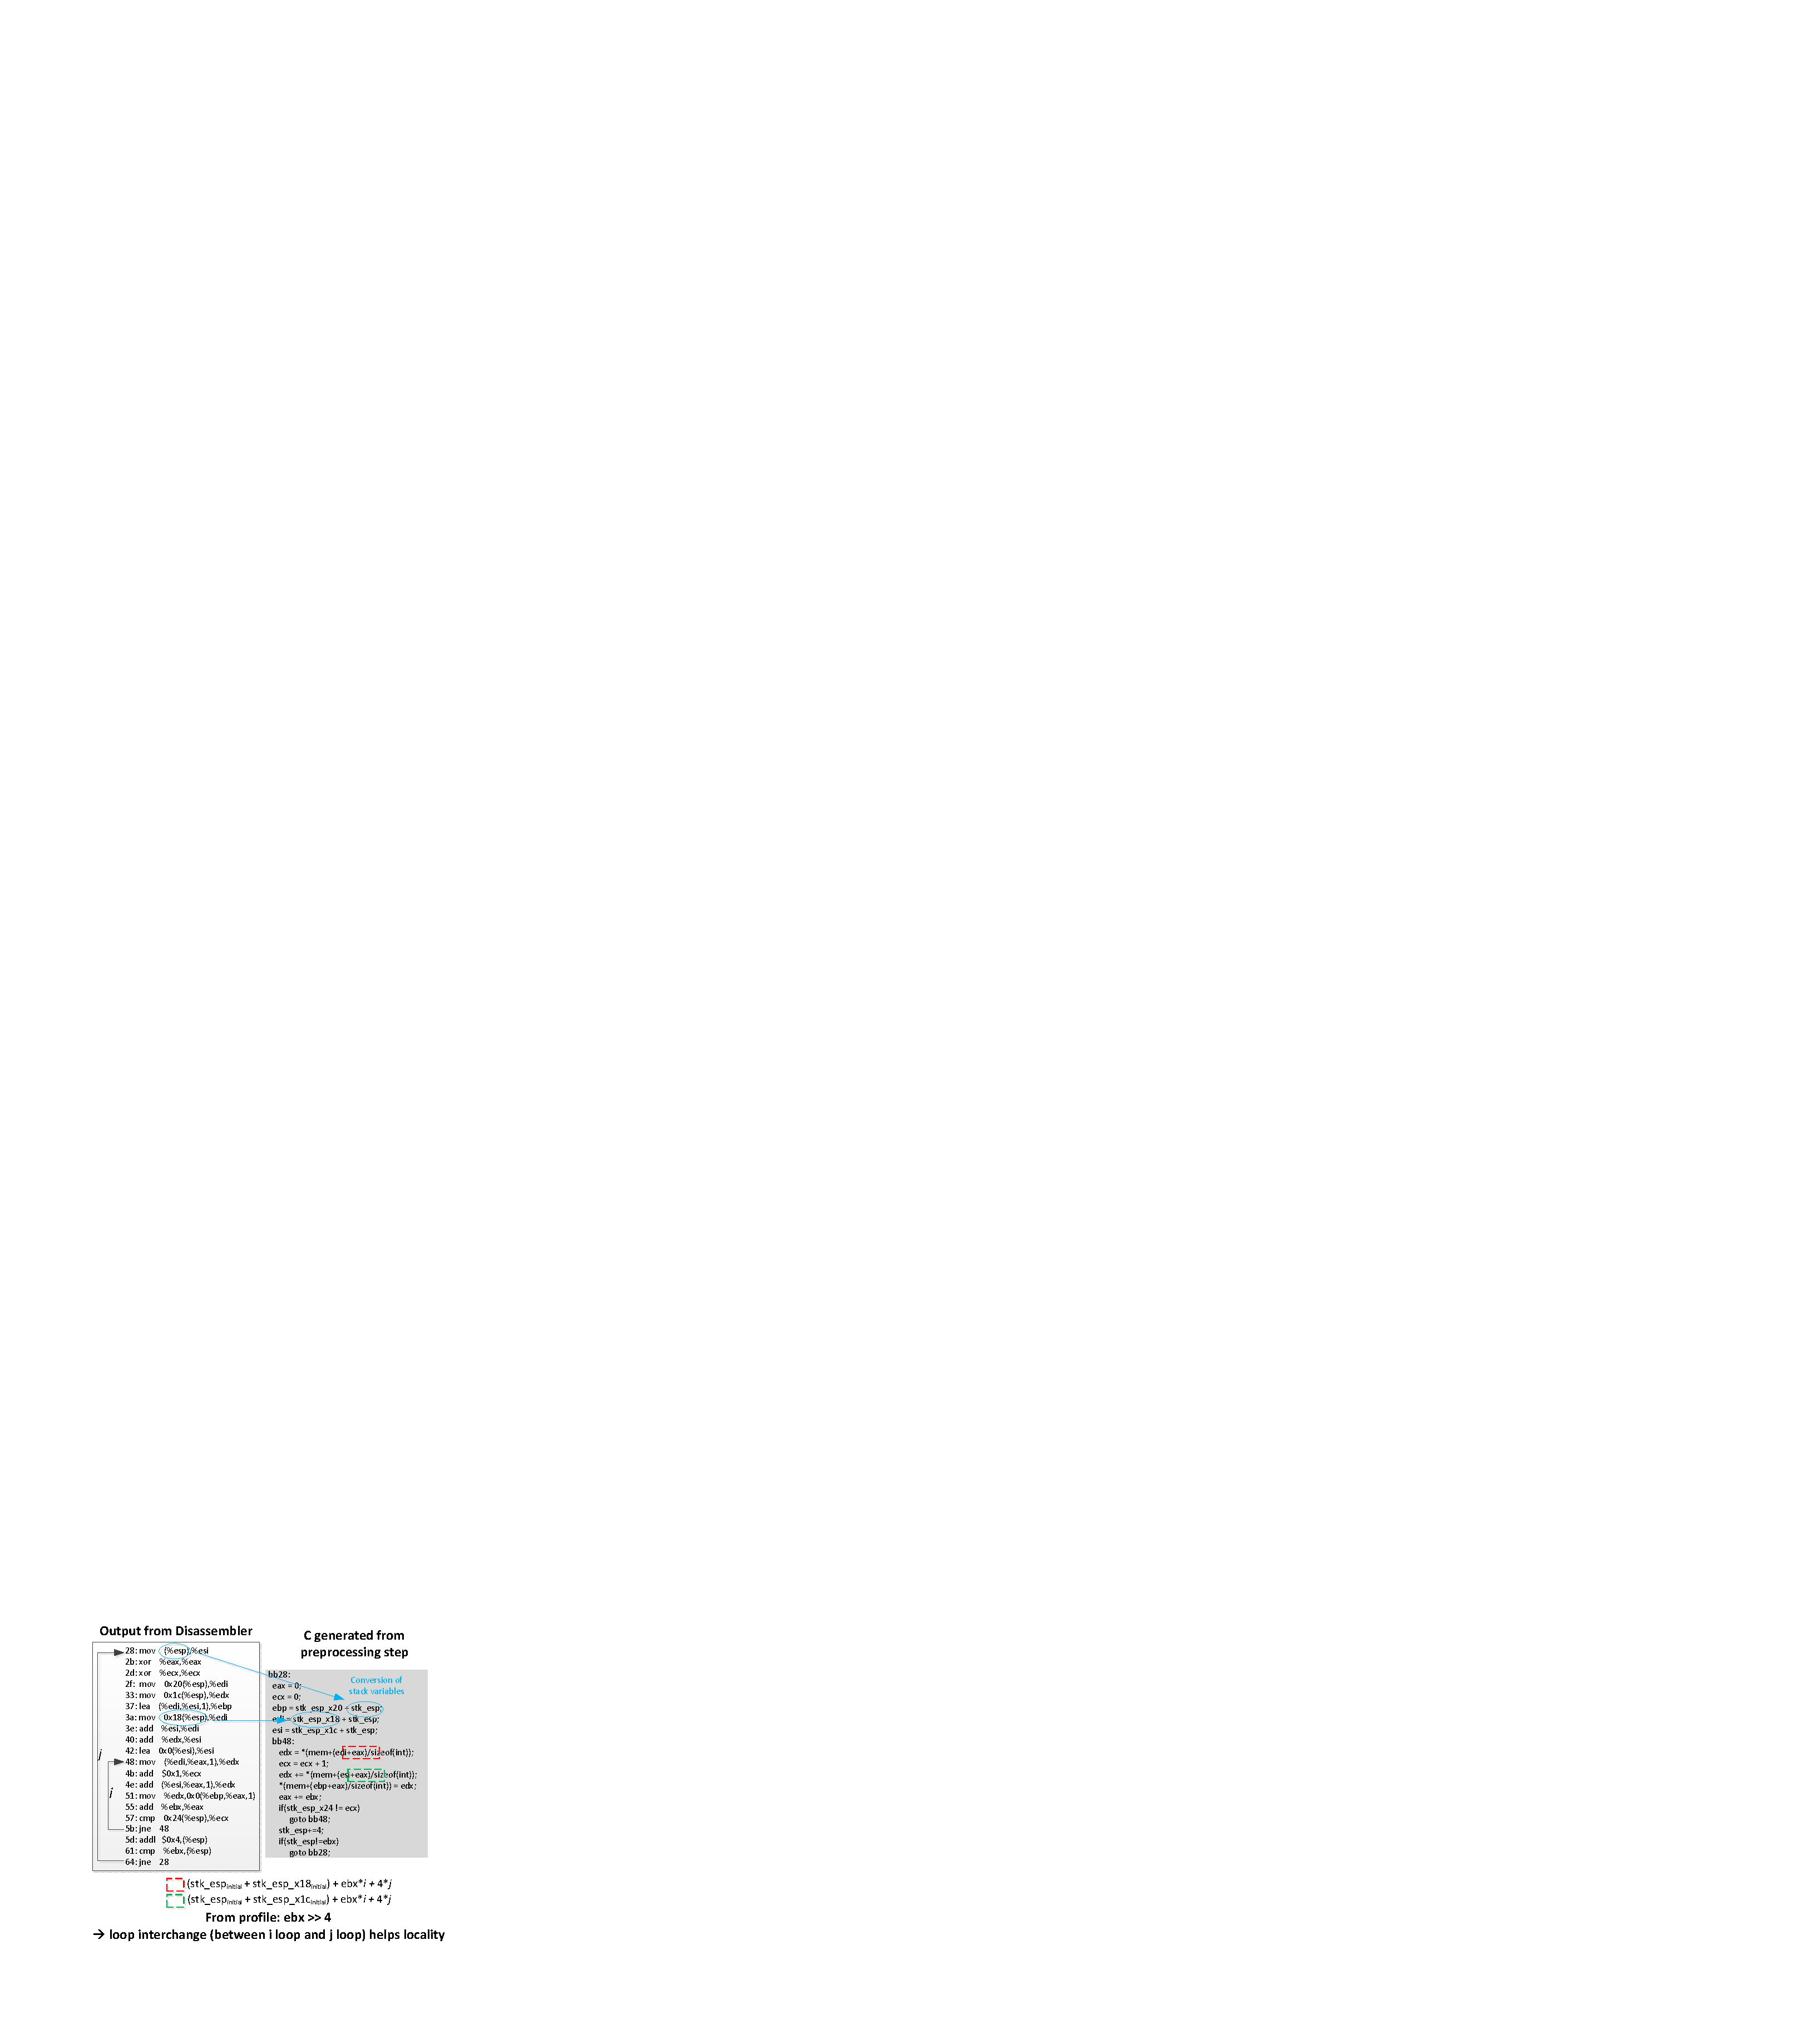
\includegraphics[width=0.8\linewidth]{chap6fig/loopInterchange.pdf}
\caption{Loop Interchange Based on Coefficient Value from Past Execution Profile 
\label{localityopt}}
\end{center}
\end{figure}

\subsection{Other Optimization for FPGA Accelerators}
While our flow exploits parallelism in 
multiple different levels, there are many other potential optimizations incorporable into our framework.  
In particular, an important factor affecting the final performance of the 
accelerator is locality of data accesses. While multiple datapaths can
easily saturate the offchip memory bandwidth, there might be wastage if opportunities for data reuse are missed. 
Even in the absence of data reuse, requests for 
contiguous segments or memory locations close to each other are more efficiently served by the caches and the memory subsystem. For programs which were written with locality in mind or compiled using toolchain capable of locality optimizations, the accelerators generated from their binaries would have already benefited  from all the techniques applied. 
In the absence of those, our approach would still allow helpful analysis and transformations to be performed during accelerator generation. 

One example would be using loop interchange to increase locality. 
%the amount of computation per unit of data communicated with off-chip RAM. 
%Thus in our flow, we also try to increase the ratio of computation per unit of data communicated with off-chip RAM. By performing loop interchange under the dependency constraints, we can generate multiple versions of a loop nest.
To generate the implementation with the smaller memory footprint (normalized by iteration count) at the inner loop level, we can leverage the run time values from the past profiles.
As the targeted loops for our flow contain memory references whose addresses are affine expressions of the loop index variables, the coefficient for each of them decides how large of a stride each iteration takes, which conveniently approximate how ``unlocal" the memory accesses are.
%For our targeted loop nests, the memory addresses accessed are affine expressions of the loop index variables. The coefficient for each of them decides how large of a stride each iteration takes, which conveniently approximate how ``unlocal" the memory accesses are. 
Thus for a particular loop index variable, the smaller the coefficient, the deeper its corresponding loop level should go. This is illustrated in figure~\ref{localityopt}. Of course, as the interchange is performed
based on past input data, for it to be valid, the resultant direction vectors can not have leading elements being $``>"$ when the accelerator is invoked with new data.
To achieve this, the $online$ phase would need to
first check if the element being moved outward is $``>"$. If it is, then we check if all the levels outside of it are $``="$. If the test result is affirmative, then the loop interchange has violated the 
original program order and the accelerator should not be invoked. %This process is illustrated in figure~\ref{}.



\begin{comment}
There are other transformations such as loop tiling and loop fission which can be 

which can be applied to extract additional parallelism or to achieve better data reuse are good additions to our flow. For each 

. Loop fission and loop tiling, for instance, are techniques used in some optimizing compilers. Their incorporation is certainly feasible with our general approach and will
add more dimensions to the design space. 


This kind of optimization can be useful
addition to our framework

The algorithm used to perform code transformation in our flow is outlined in algorithm~\ref{algoPara}. This is a modified version of the \textit{codegen}
procedure from~\cite{Kennedy:2001:OCM:502981}, which targets vector machines.
Our implementation, in addition to data level parallelism, also try to expose
thread level parallelism at the outer level loop, which can then be exploited by multiple FPGA datapaths. 
The results from our algorithm only provides a starting point for the design space exploration. Even for a single vectorized instruction, combinations of techniques illustrated in figure~\ref{fig:fpgaparal} can be applied to
produce implementations of different performance area trade-off. Meanwhile, 
the supporting infrastructure on the FPGA can also be modified on a per
application basis. The parametrization of on-chip buffer, communication mechanism with external
storage etc. are all parts of the design space. The co-tuning of these ``glue"
structures in conjunction
with the accelerator itself is left to future work.  In section~\ref{biev}, we sample a small subset of the possible design points
to show the trade-off between different metrics.
\end{comment}

There are also other transformations which can be applied to extract additional parallelism or to achieve better data reuse. Loop fission and loop tiling, for instance, are techniques used in some optimizing compilers. 
Their incorporation is certainly feasible with our general approach and will
add more dimensions to the design space. 



\begin{comment}

For loop interchange to be valid, the resultant direction vectors would need to have
leading elements not being $``>"$. To achieve this, we first check if the element being moved outward is $``>"$. If it is, then we check if all the levels outside of it are $``="$. If the test result is affirmative, then the loop interchange has violated the 
original program order and the accelerator should not be invoked. This process
is illustrated in figure~\ref{}.



%When the input data are changed, the generated accelerator may actually violate
%the semantics of the program. As we have mentioned in section~\ref{sec:cfbba},
%a verifying function is invoked before the accelerator to ensure the correctness
%of the overall execution. Besides, the \textit{online} phase also need to 



%Now the dependency testing results and the subsequent parallelization are a reflection of the programs' past behavior which
%may or may not hold true when the input data are changed. This is when the
%second phase 






%To actually obtain the direction vectors from equation~\ref{adioeq},
%we use Banerjee's approach~\cite{banerjee}.
%To actually solve equation~\ref{adioeq}, we use Banerjee's approach~\cite{}, which find the solution for the non-integer relaxation of the ILP formulation. It does
%which requires constant coefficients. 
%As the coefficients in the equation are not known from the static binary, our flow examines the runtime profiles to extract the values.
%The direction vectors thus obtained can be used evaluate how much coarse
%grained parallelism 



%Their values are extracted from the runtime profile of the programs.
Therefore, the dependency testing results are a reflection of the programs'
past behavior, which may or may not hold true when the input data are changed.
However, given a new set of runtime variables, the amount of computation needed to confirm the results of earlier dependency testing would be constant. This is not hard to see as the size of the problem formulated 
does not depend on the actual values of the coefficients. We now have the computation which has $O(1)$ cost yet guarantees the validity of the extracted
parallelism.


Meanwhile, it is worth noting that Banerjee's inequality only tests for existence of \textit{ real} solutions for the Diophantine's equations. Since it only tackles the non-integer relaxation of the ILP formulation, the results obtained are conservative. False dependencies are reported if all the real solutions are non-integral. More accurate tests like~\cite{omega} find integer solutions but are more costly. As we are
going to perform the test using runtime data when the accelerator is actually
being invoked, the faster, though more pessimistic, approach is preferred.





To actually obtain the direction vectors from equation~\ref{adioeq},
we use Banerjee's approach~\cite{banerjee}.
%To actually solve equation~\ref{adioeq}, we use Banerjee's approach~\cite{}, which find the solution for the non-integer relaxation of the ILP formulation. It does
%which requires constant coefficients. 
As mentioned in section~\ref{sec:cfbba}, the coefficients in the equation, despite being unchanged during the loop execution, are not known from the static binary. Our flow examines the runtime profiles to extract the coefficient values
%Their values are extracted from the runtime profile of the programs.
Therefore, the dependency testing results are a reflection of the programs'
past behavior, which may or may not hold true when the input data are changed.
However, given a new set of runtime variables, the amount of computation needed to confirm the results of earlier dependency testing would be constant. This is not hard to see as the size of the problem formulated 
does not depend on the actual values of the coefficients. We now have the computation which has $O(1)$ cost yet guarantees the validity of the extracted
parallelism.


Meanwhile, it is worth noting that Banerjee's inequality only tests for existence of \textit{ real} solutions for the Diophantine's equations. Since it only tackles the non-integer relaxation of the ILP formulation, the results obtained are conservative. It will never report lack of dependencies when one exists,  but may report false dependencies -- when all the real solutions are non-integral. More accurate tests like~\cite{omega} find integer solutions but are more costly. As we are
going to perform the test using runtime data when the accelerator is actually
being invoked, the faster, though more pessimistic, approach is preferred.







As we mentioned in section~\ref{sec:cfbba}, for loops with analyzable memory accesses, we can perform run time check to validate parallelization we performed in creating the accelerators. This 

As we use past execution profiles to extract parallelism and then perform runtime checks to confirm the validity of our parallelization, our approach
in accelerating program binaries can be divided into two phases. The offline
phase (compile time) consists of dependency analysis, accelerator synthesis and accelerator driver generation. Meanwhile, the parallelism validity check, data transfer and invocation of the accelerator are all performed during the online phase (run time). Being part of the driver, the actual code segments to perform validity check and data transfer are all generated during compile time. As our primary objective is to boost the performance of the accelerated loop nests, the flow tries to create simple and fast run time code whenever it, at the expense
of the compilation time and at times, the accuracy of the run time mechanisms.
\end{comment}